\documentclass[]{article}
\usepackage[a4paper, margin=2cm]{geometry}
\usepackage{amsmath}
\usepackage{amsfonts}
\usepackage{amssymb}
\usepackage{mathtools}
\usepackage{amsthm}
\usepackage[many]{tcolorbox}
\usepackage{listings}
\usepackage{cancel}
\usepackage{graphicx}
\usepackage{subfigure}
\usepackage{hyperref}
\usepackage{biblatex}

\newtheorem{lemma}{Lemma}
\newtheorem{theorem}{Theorem}
\newtheorem{definition}{Definition}
\newtheorem{algorithm}{Algorithm}
\newtheorem{example}{Example}
\newtheorem{remark}{Remark}
\newtheorem{recap}{Recap}
\newtheorem{corollary}{Corollary}


\tcolorboxenvironment{lemma}{
	colback=yellow!5!white,
	boxrule=0pt,
	boxsep=1pt,
	left=2pt,right=2pt,top=2pt,bottom=2pt,
	oversize=2pt,
	sharp corners,
	before skip=\topsep,
	after skip=\topsep,
}

\tcolorboxenvironment{theorem}{
	colback=yellow!5!white,
	boxrule=0pt,
	boxsep=1pt,
	left=2pt,right=2pt,top=2pt,bottom=2pt,
	oversize=2pt,
	sharp corners,
	before skip=\topsep,
	after skip=\topsep,
}

\tcolorboxenvironment{definition}{
	colback=green!5!white,
	boxrule=0pt,
	boxsep=1pt,
	left=2pt,right=2pt,top=2pt,bottom=2pt,
	oversize=2pt,
	sharp corners,
	before skip=\topsep,
	after skip=\topsep,
}


\begin{document}
	
	\title{Computer Aided Geometric Design Compendium WS2023}
	\author{Ida Hönigmann}
	
	\maketitle

\section*{Organization}
Lecture each Thursday 12:00 to 14:00 (full 2 hours).
\\
Oral exam. Write email to fix date and time.
\\
Problem session each Thursday 14:00 to 16:00. Mandatory attendance!
\\
Kreuzerlübung.

\section{Bezier curves}

\begin{example}
	\begin{figure}[h!]
		\subfigure{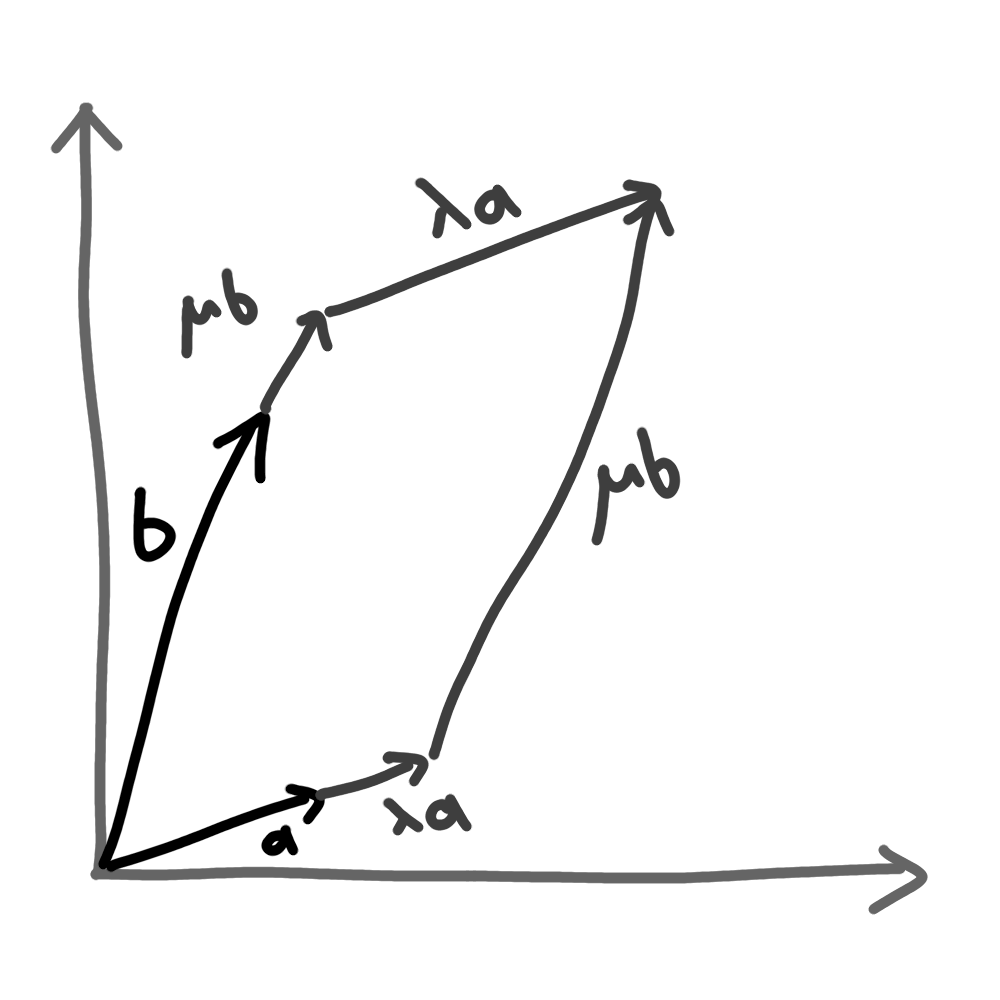
\includegraphics[width=0.3\linewidth]{figures/linear_combination_example}} 
		\subfigure{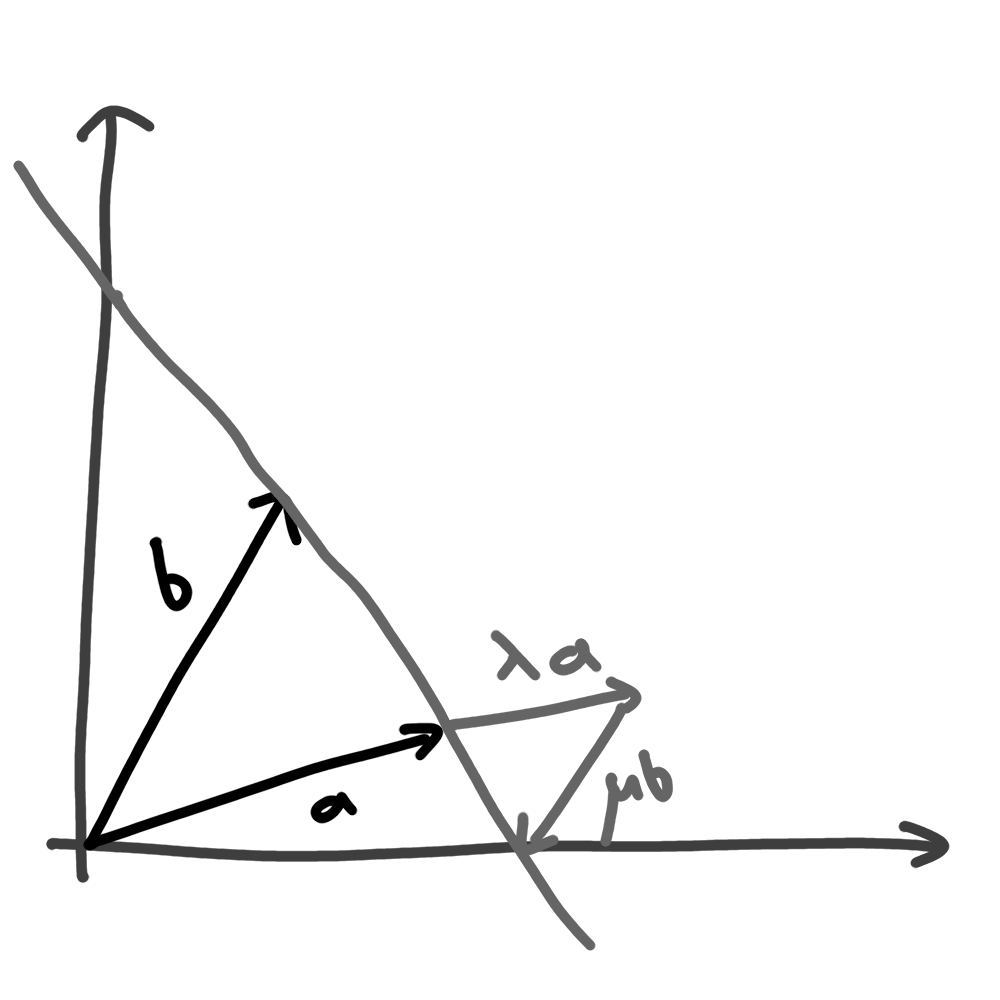
\includegraphics[width=0.3\linewidth]{figures/affine_combination_example}} 
		\subfigure{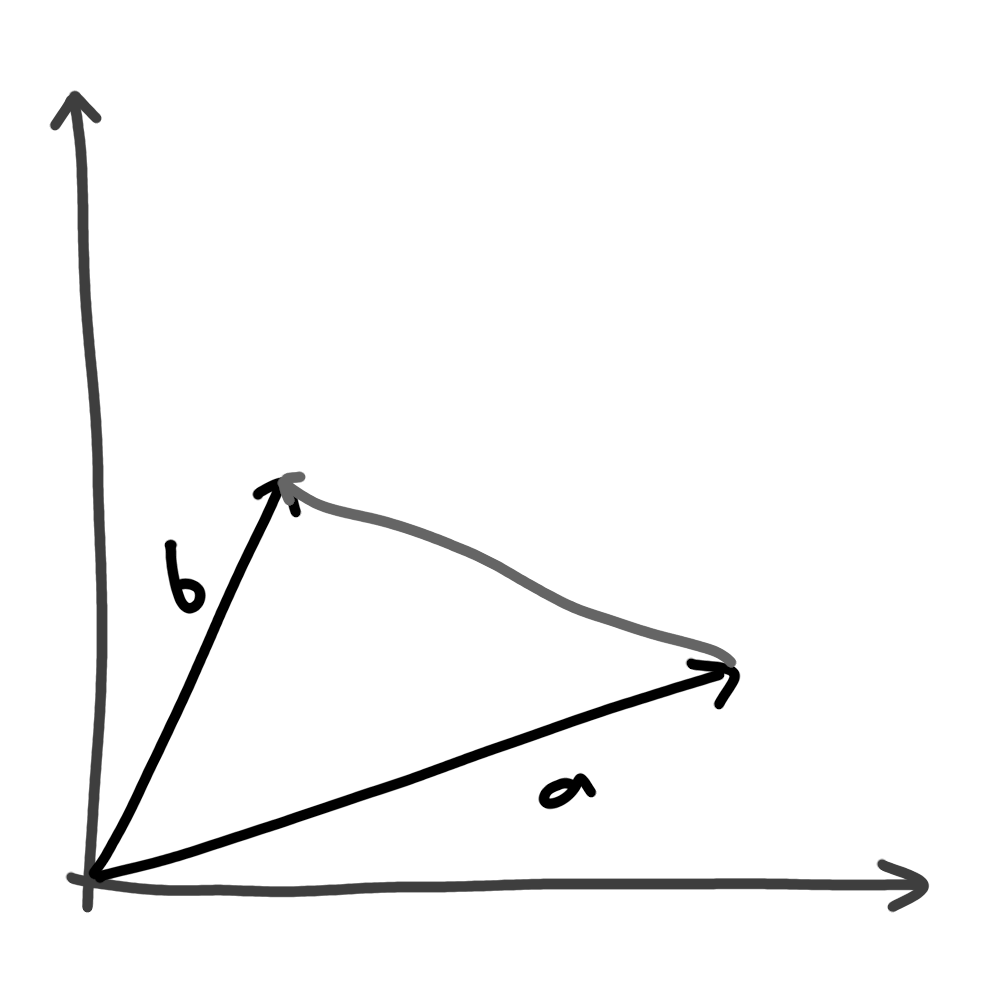
\includegraphics[width=0.3\linewidth]{figures/convex_combination_example}} 
		\caption{Linear combination, affine combination and convex combination}
		\label{fig:combinationexample}
	\end{figure}
	
	\textbf{Linear combination} $\lambda a + \mu b$

	\textbf{Affine combination} $\lambda a + \mu b$ and $\lambda + \mu = 1$
	
	What is $\mu$ so that $\lambda a + \mu B$ is on the line?
	\begin{align*}
		\lambda a + \mu b = a + t(b-a) \implies a (\underbrace{\lambda - 1 + t}_{=0}) + b (\underbrace{\mu - t}_{=0}) = 0
	\end{align*}
	If $a,b$ are linearly independent $\implies \mu = t \land \lambda + \mu = 1$

	\textbf{Convex combination} $\lambda a + \mu b$ and $\lambda + \mu = 1$ and $\lambda,\mu \geq 0$
	
	Line is $a + t(b-a)$ with $t\in[0,1]$ $\implies \mu,\lambda \in [0,1]$
\end{example}

\begin{definition}[combinations]
	linear combination $\sum_{i=1}^{n} \lambda_i v_i$ with $v_1,...,v_n \in \mathbb{R}^d, \lambda_1,...,\lambda_n \in \mathbb{R}$
	
	affine combination $\sum_{i=1}^{n} \lambda_i v_i$ with $\sum_{i=1}^{n} \lambda_i = 1$
	
	convex combination $\sum_{i=1}^{n} \lambda_i v_i$ with $\sum_{i=1}^{n} \lambda_i = 1$ and $\forall i: \lambda_i \geq 0$
\end{definition}

\begin{algorithm}[of de Casteljou, Bezier curve]
	Given: $b_0,...,b_n \in \mathbb{R}^d$ (called control points / Kontrollpunkte), $t \in \mathbb{R}$
	\\Recursion: $b_i^0(t) := b_i$
	\\$b_i^j(t) := (1-t)b_i^{j-1}(t) + tb_{i+1}^{j-1}(t)$ for $j=1,...,n$ and $i=0,...,n-j$
	\\Result: $b(t):=b_0^n(t)$ (called Bezier curve)
	
\end{algorithm}

\begin{remark}
	In the algorithm above often we choose $t\in[0,1]$.
\end{remark}

\begin{example}
	\begin{figure}[h!]
		\subfigure{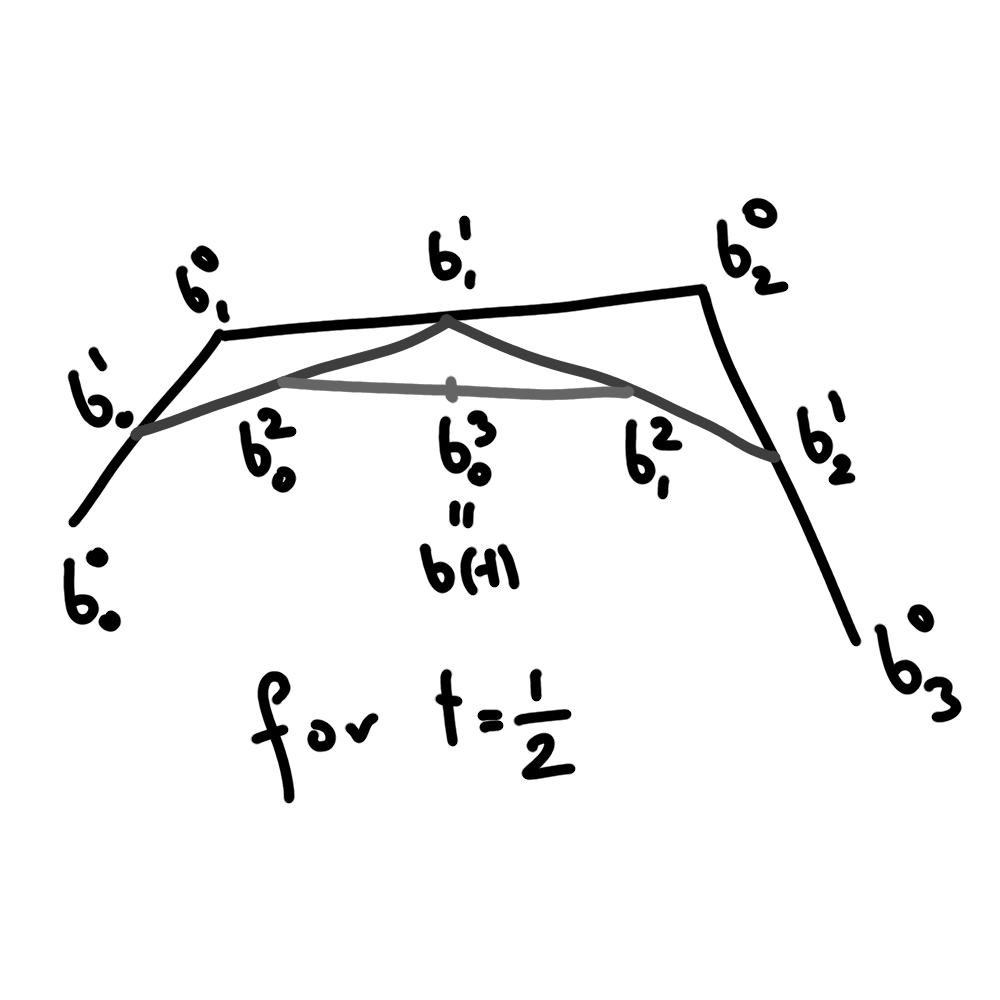
\includegraphics[width=0.3\linewidth]{figures/decasteljou_example_1}} 
		\subfigure{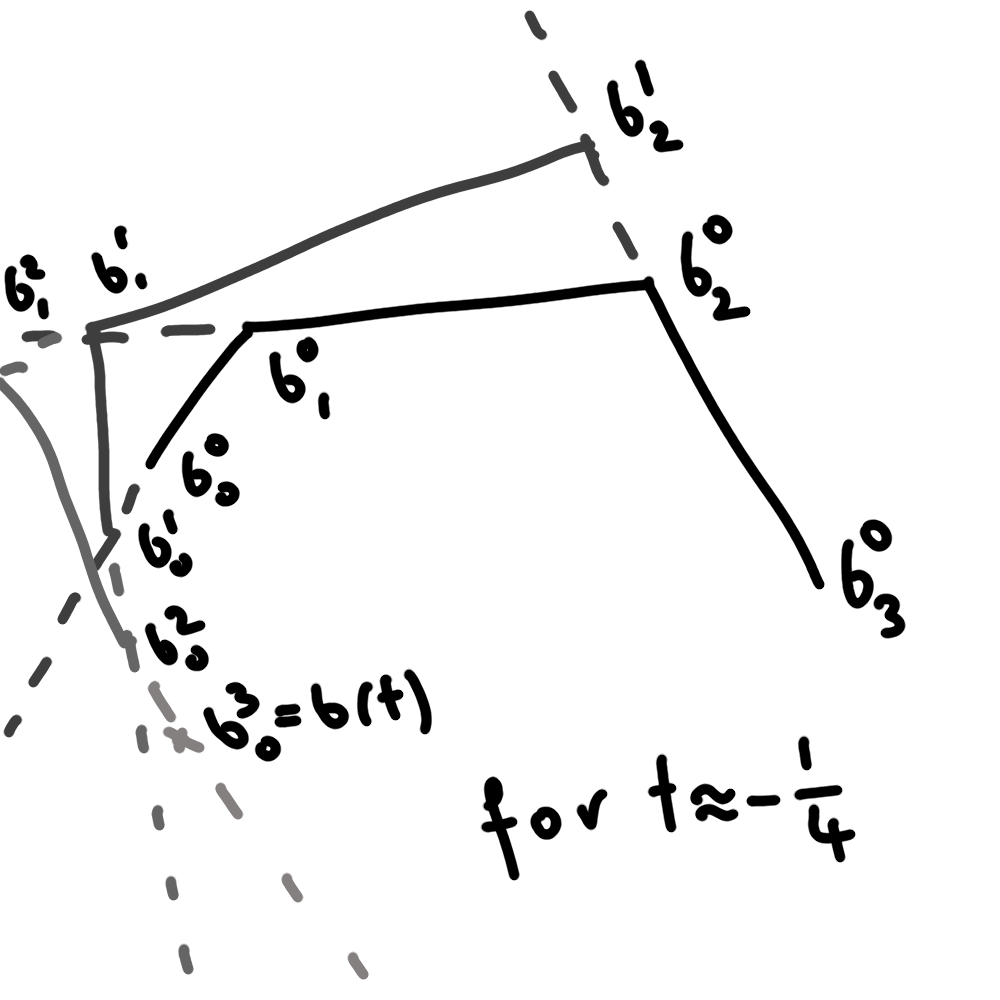
\includegraphics[width=0.3\linewidth]{figures/decasteljou_example_2}} 
		\subfigure{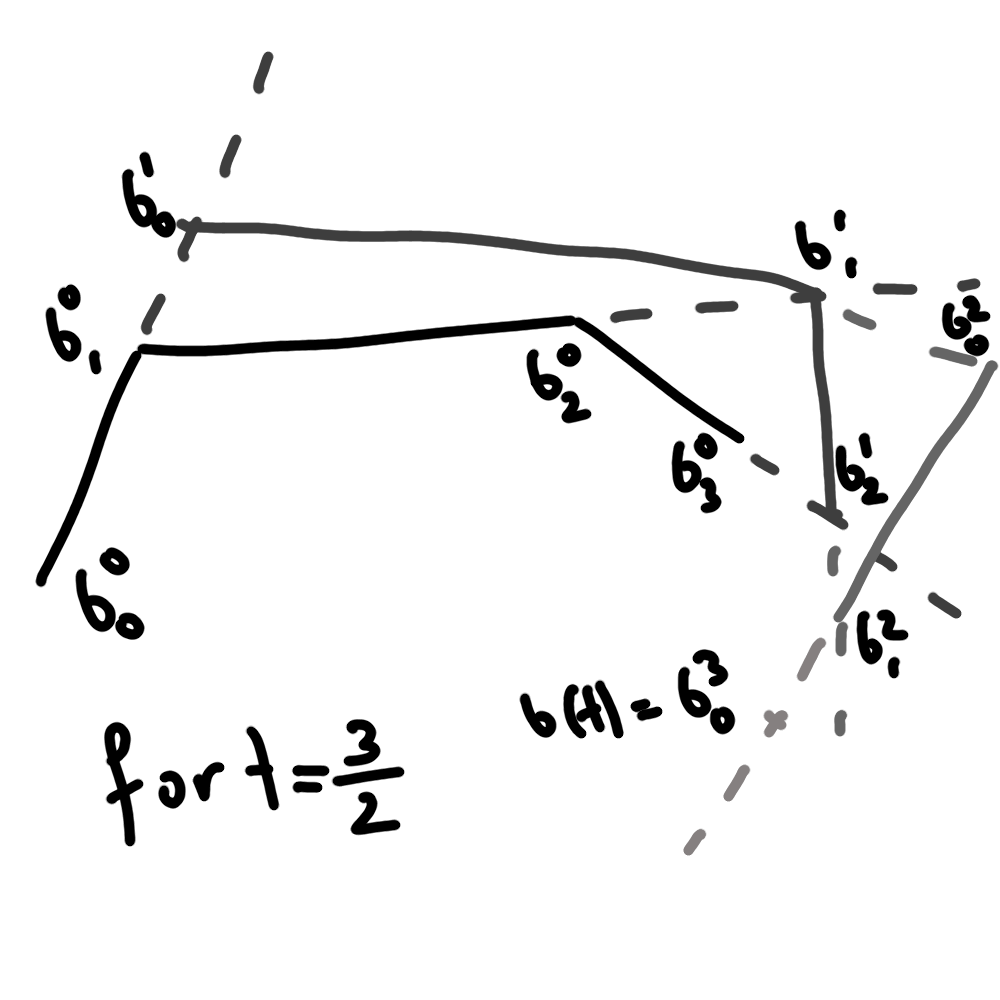
\includegraphics[width=0.3\linewidth]{figures/decasteljou_example_3}} 
		\caption{Examples of the de casteljou algorithm}
		\label{fig:decasteljouexample}
\end{figure}
\end{example}

\begin{remark}
	In this course $\mathbb{N}=\{1,2,3,...\}$ and $\mathbb{N}_0=\{0,1,2,3,...\}$
\end{remark}

\begin{recap}
	$0! := 1, n! := n(n-1)(n-2) \cdots 1$ for $n \geq 1$.
	
	\begin{align*}
		\binom{n}{k} := \begin{cases}
			\frac{n!}{k!(n-k)!}&, n\geq k \geq 0\\
			0&, k > n
		\end{cases} \text{ for } n,k \in \mathbb{N}_0
	\end{align*}
\end{recap}

\begin{definition}[Bernstein polynomials]
	For $n,i \in \mathbb{N}_0$ we define $B_i^n(t) := \binom{n}{i} t^i (1-t)^{n-i} \in \mathbb{R}[t]$
\end{definition}

\begin{remark}
	Special cases of Bernstein polynomials
	
	\begin{align*}
		i > n \implies B_i^n(t) = 0 && B_i^n(0) = \begin{cases}0, i\not= 0\\ 1, i=0 \end{cases} \\
		B_i^n(1) = \begin{cases}0, i\not= n\\ 1, i=n \end{cases} && B_0^0(t) = 1
	\end{align*}
\end{remark}

\begin{theorem}
	$b_i^j(t) = \sum_{l=0}^{j} B_l^j(t) b_{i+l}$
\end{theorem}

\begin{proof}
	Induction over $j$: $j=0$:
	\begin{align*}
		j=0: && b_i^0(t):= b_i = 1 \cdot b_i = B_0^0(t) \cdot b_i \hspace{1cm} \checkmark\\
		j-1 \rightarrow j: && b_i^j(t) := (1-t)b_i^{j-1}(t) + t b_{i+1}^{j-1}(t) \overset{\mathrm{IA}}{=}
		(1-t) \sum_{l=0}^{j-1} B_l^{j-1}(t) b_{i+l} + t \sum_{l=0}^{j-1} B_l^{j-1}(t) b_{i+1+l} =\\
		&& (1-t) \sum_{l=0}^{\overset{j}{\cancel{j-1}}} B_l^{j-1}(t) b_{i+l} + t \sum_{l=\underset{0}{\cancel{1}}}^{j} B_{l-1}^{j-1}(t) b_{i+l} =
		\sum_{l=0}^{j} (\underbrace{(1-t) B_l^{j-1}(t) + t B_{l-1}^{j-1}(t)}_{=B_l^j(t) \text{ using the following lemma}}) b_{i+l} =\\
		&& \sum_{l=0}^{j} B_l^j(t) b_{i+l} \hspace{1cm} \checkmark
	\end{align*}
\end{proof}

\begin{corollary}
	The Bezier curve equals $b(t) = b_0^n(t) = \sum_{l=0}^{n} B_l^j(t) b_{i+l}$, which is called the Bernstein representation of the Bezier curve.
\end{corollary}

\begin{remark}
	As $b(t) = \sum_{l=0}^{n} B_l^n(t) b_l \in C^\infty$ it is a polynomial curve of degree $n$, which is in $C^\infty$ and therefore ''very smooth''.
\end{remark}

\begin{lemma}
	$B_l^j(t) = (1-t)B_l^{j-1}(t) + t B_{l-1}^{j-1}(t)$
\end{lemma}

\begin{proof}
	\begin{align*}
		(1-t)B_l^{j-1}(t) + t B_{l-1}^{j-1}(t) = (1-t) \binom{j-1}{l} t^l (1-t)^{j-1-l} + t \binom{j-1}{l-1} t^{l-1} (1-t)^{j-1-l+1} =\\
		\binom{j-1}{l} t^l (1-t)^{j-l} + \binom{j-1}{l-1} t^{l} (1-t)^{j-l} = \left(\binom{j-1}{l} + \binom{j-1}{l-1}\right) t^l (1-t)^{j-l} = \binom{j}{l} t^l (1-t)^{j-l} = B_l^j(t)
	\end{align*}
\end{proof}

\begin{remark}
	What is $b(0)$? \hspace{1cm} $b(0)=\sum_{i=0}^{n} B_i^n(0) b_i = b_0 + 0 + 0 + \cdots + 0 = b_0$\\
	What is $b(1)$? \hspace{1cm} $b(1)=\sum_{i=0}^{n} B_i^n(1) b_i = 0 + \cdots + 0 + b_n = b_n$
\end{remark}

\begin{definition}[end-point-interpolating]
	Curves which pass through the first and last point are called end-point-interpolating (Endpunktinterpolierend).
\end{definition}

\begin{remark}
	Bezier curves are end-point-interpolating.
\end{remark}

\begin{remark}
	How many intersection points are there between a planar (i.e. in $\mathbb{R}^2$) Bezier curve and a straight line?
	\begin{align*}
		\text{Straight line: } p + t(q-p) && \text{ Bezier curve: } b(t) = \sum_{i=0}^{n} B_i^n(t) \underbrace{b_i}_{\in \mathbb{R}^2}
	\end{align*}
	
	Solving $p+t(q-p) = \sum_{i=0}^{n} B_i^n(t) b_i$ results in at most $n$ solutions.
\end{remark}

\begin{lemma}
	$\frac{d}{dt}B_i^n(t) = n(B_{i-1}^{n-1}(t) - B_i^{n-1}(t))$
\end{lemma}

\begin{proof}
	\begin{align*}
		\frac{d}{dt}B_i^n(t) = \frac{d}{dt} \binom{n}{i} t^i (1-t)^{n-i} = \binom{n}{i} i t^{i-1} (1-t)^{n-i} - \binom{n}{i} t^i (n-i) (1-t)^{n-i-1} =\\
		\frac{n!}{\underset{(i-1)!}{\cancel{i!}}(n-i)!} \cancel{i} t^{i-1} (1-t)^{n-i} - \frac{n!}{i!\underset{(n-i-1)!}{\cancel{(n-i)!}}}\cancel{(n-i)}t^i (1-t)^{n-i-1} =\\
		n \left(\frac{(n-1)!}{(i-1)!(n-i)!}t^{i-1}(1-t)^{n-i} - \frac{(n-1)!}{i!(n-i-1)!} t^i (1-t)^{n-i-1}\right) =\\
		n \left(\binom{n-1}{i-1}t^{i-1}(1-t)^{n-i} - \binom{n-1}{i} t^i (1-t)^{n-i-1}\right) = n(B_{i-1}^{n-1}(t) - B_i^{n-1}(t))
	\end{align*}
\end{proof}

\begin{theorem}
	$\dot{b}(t) := \frac{d}{dt} b(t) = n \sum_{i=0}^{n-1} B_i^{n-1}(t)(b_{i+1} - b_i) = n (b_1^{n-1}(t) - b_0^{n-1}(t))$
\end{theorem}

\begin{proof}
	\begin{align*}
		\dot{b}(t) = \frac{d}{dt} \left(\sum_{i=0}^{n} B_i^n(t) b_i\right) = \sum_{i=0}^{n} \frac{d}{dt} B_i^n(t) b_i = \sum_{i=0}^{n} n(B_{i-1}^{n-1}(t) - B_i^{n-1}(t)) b_i = n \left(\sum_{i=0}^{n} B_{i-1}^{n-1}(t) b_i - \sum_{i=0}^{n} B_i^{n-1}(t) b_i\right) =\\
		n \left(\sum_{i=1}^{n} B_{i-1}^{n-1}(t) b_i - \sum_{i=0}^{n} B_i^{n-1}(t) b_i\right) = n\left(\underbrace{\sum_{i=0}^{n-1} B_i^{n-1}(t) b_{i+1}}_{=b_1^{n-1}(t)} - \underbrace{\sum_{i=0}^{n-1} B_i^{n-1}(t) b_i}_{=b_0^{n-1}(t)}\right) = n \left(\sum_{i=0}^{n-1} B_i^{n-1}(t)(b_{i+1} - b_i)\right)
	\end{align*}
\end{proof}

\begin{corollary}
	\begin{itemize}
		\item $\dot{b}(0) = n (b_1 - b_0)$
		\item $\dot{b}(1) = n (b_n - b_{n-1})$
		\item The last segment in the algorithm of de Casteljou is the tangent of the Bezier curve in $b(t)$.
		\item The derivative of a bezier curve of degree $n$ is a bezier curve of degree $n-1$ with control points $(b_1,b_0), (b_2 - b_1), \cdots, (b_n - b_{n-1})$.
	\end{itemize}
\end{corollary}

\begin{corollary}
	$\ddot{b}(t) = n (n-1) \sum_{i=0}^{n-2} B_i^{n-2}(t) (b_{i+2} - 2 b_{i+1} + b_i)$
	
	$\ddot{b}(0) = n(n-1)(b_2 - 2b_1 + b_0)$, $\ddot{b}(1) = n(n-1)(b_n - 2b_{n-1} + b_{n-2})$
\end{corollary}

\begin{corollary}
	The curvature of a bezier curve in the point $b(0)$ depends only on $b_0, b_1, b_2$.
	
	The curvature of a bezier curve in the point $b(1)$ depends only on $b_{n-2}, b_{n-1}, b_n$.
\end{corollary}

\begin{example}
	Quadratic Bezier curve
	\begin{align*}
		b(t) = \sum_{i=0}^{2} B_i^2(t) b_i = \binom{2}{0} t^0 (1-t)^2 b_0 + \binom{2}{1} t^1 (1-t)^1 b_1 + \binom{2}{2} t^2 (1-t)^0 b_2 = t^2(b_2-2b_1+b_0) + t(2b_1 - 2b_0) + b_0
	\end{align*}
	which is an affine transformation of a parabola and therefore a parabola.
	
	Quadratic bezier curves are parabolas.
\end{example}

\begin{remark}
	Line at infinity (Ferngerade) is the collection of points where parallel lines intersect.
	
	\begin{figure}[h!]
		\centering
		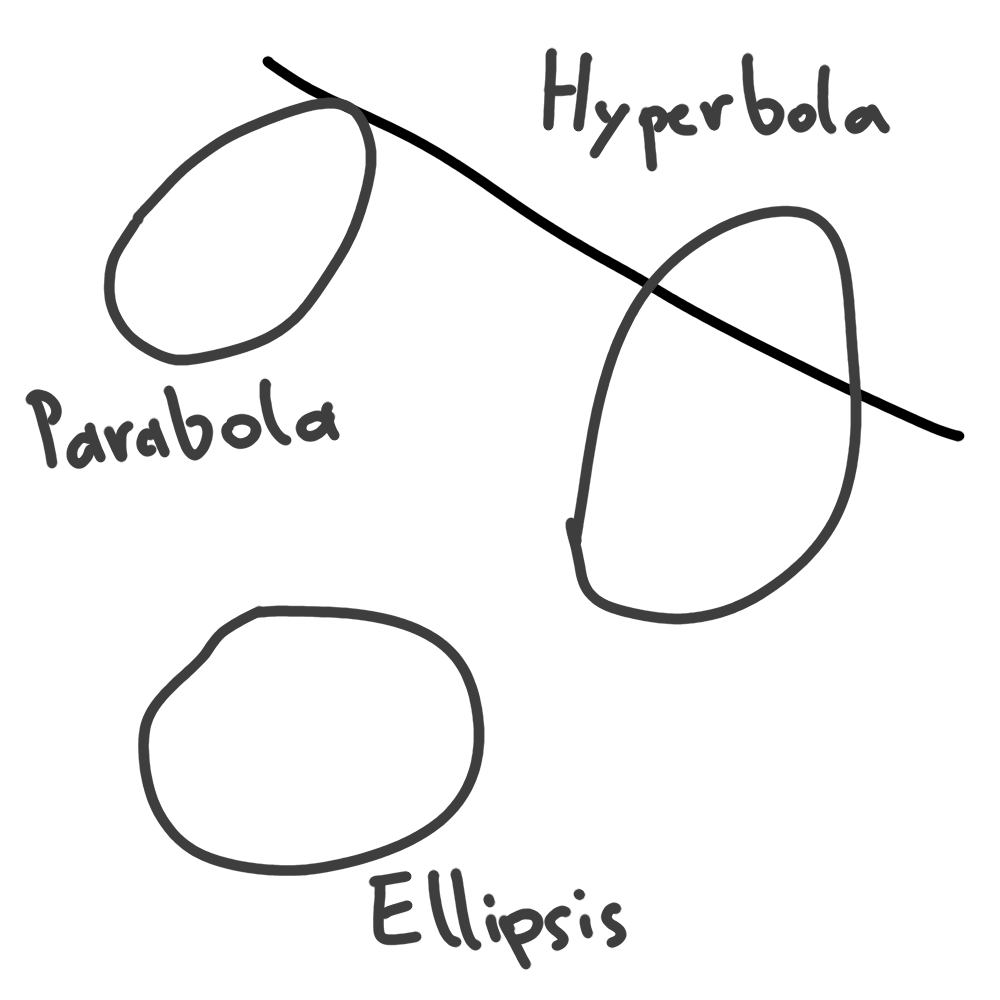
\includegraphics[width=0.3\linewidth]{figures/line_at_infinity}
		\caption{Categorization of Parabolas, Hyperbolas and Ellipsis as intersection points with the line at infinity.}
		\label{fig:lineatinfinity}
	\end{figure}
	
\end{remark}

\begin{remark}
	Different applications using these curves are Rhino, OpenSCAD, Autocad, Geogebra, ...
\end{remark}



\section{Parameterized curves}

\begin{figure}[h!]
	\centering
	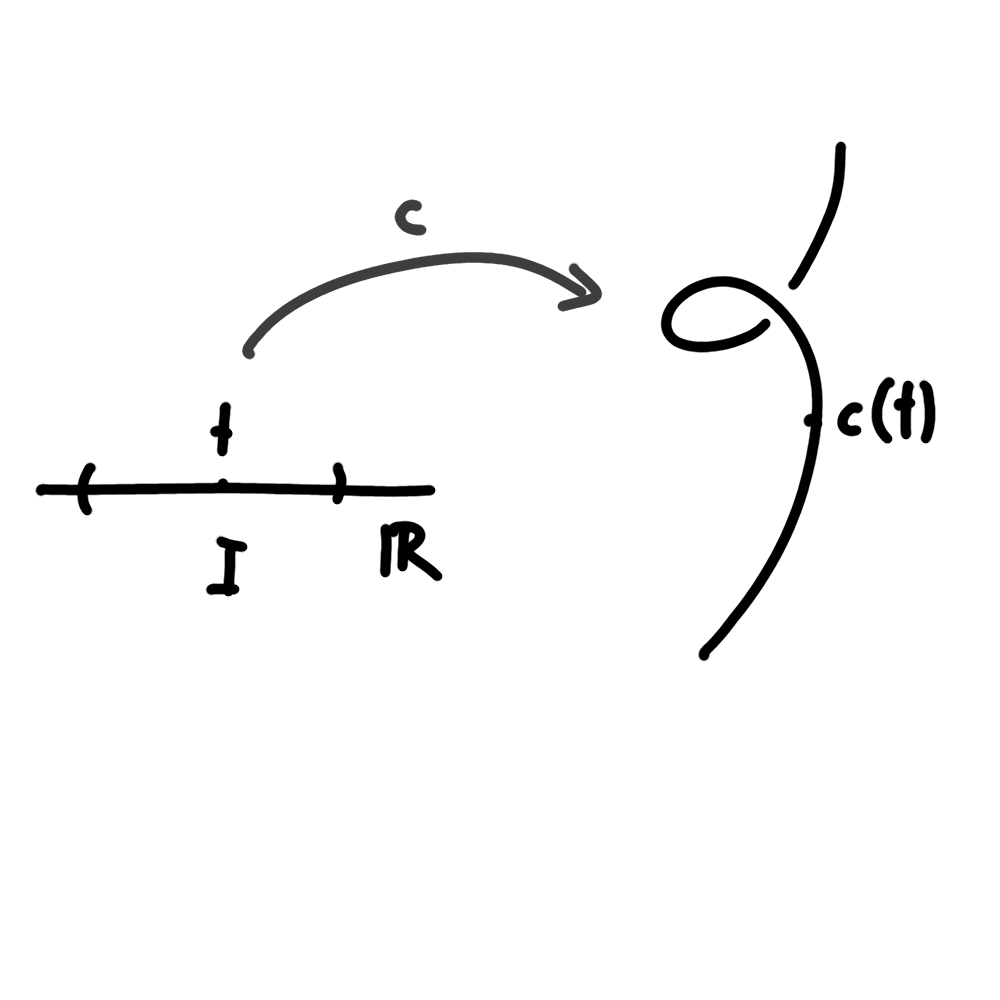
\includegraphics[width=0.3\linewidth]{figures/parameterized_curve}
	\caption{parameterized curve $c(t)$}
	\label{fig:parameterizedcurve}
\end{figure}

\begin{definition}
	$c:I\subseteq \mathbb{R} \rightarrow \mathbb{R}^3$ is called a parameterized curve.
	 
	
	$\dot{c}(t) := \frac{d}{dt} c(t)$ is called the tangential vector. For $\mathbb{R}^3$ we have $\dot{c}(t) = (\dot{c_1}(t), \dot{c_2}(t), \dot{c_3}(t))$.

	The velocity is defined as $|| \dot{c}(t) ||$.
	
	A point $c(t)$ is called regular, if $\dot{c}(t) \not= 0$ and is called singular, if $\dot{c}(t) = 0$.
\end{definition}

\begin{example}
	A helix (Schraublinie) is defined by $c(t) = (\cos(t), \sin(t), t)^T$.
	
	\begin{figure}[h!]
		\centering
		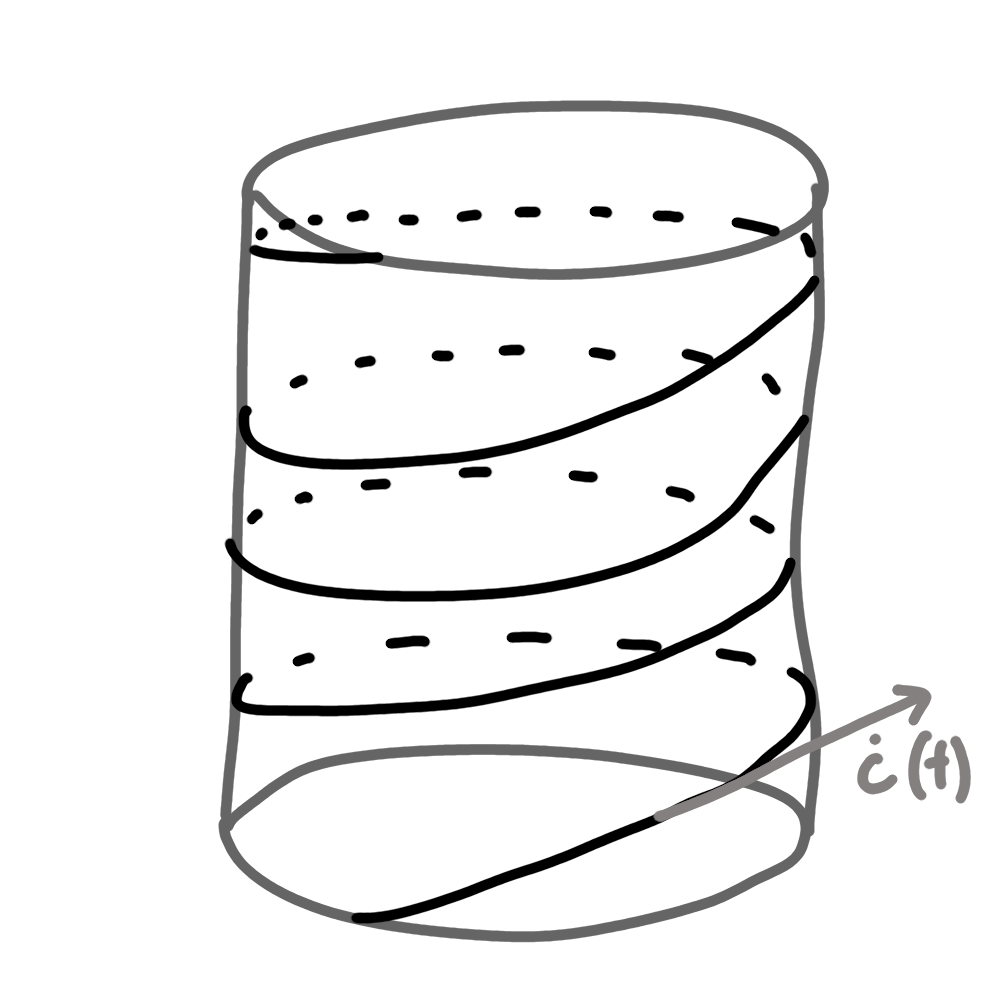
\includegraphics[width=0.3\linewidth]{figures/helix}
		\caption{Helix with tangential vector}
		\label{fig:helix}
	\end{figure}
	
	\begin{align*}
		\dot{c}(t) = (-\sin(t), \cos(t), 1)^T && ||\dot{c}(t)|| = \sqrt{\sin^2(t) + \cos^2(t) + 1} = \sqrt{2}
	\end{align*}
	
	We see that the helix is passed through with constant velocity. Furthermore all points are regular.
\end{example}

\begin{example}
	$c:\mathbb{R} \rightarrow \mathbb{R}^3, t \mapsto (t^2, t^3, t^4)$, $\dot{c}(t) = (2t, 3t^2, 4t^3)$. We see that $0$ is singular as $\dot{c}(0) = (0, 0, 0)$. Everywhere else the curve is regular.
\end{example}

\begin{remark}
	A point being regular or singular depends on the parameterisation of the curve.
	
	For example $c(t) = (t,t)$ produces a regular curve, while $c(t) = (t^3, t^3)$ produces a curve where $0$ is singular.
	
	
	\begin{figure}[h!]
		\centering
		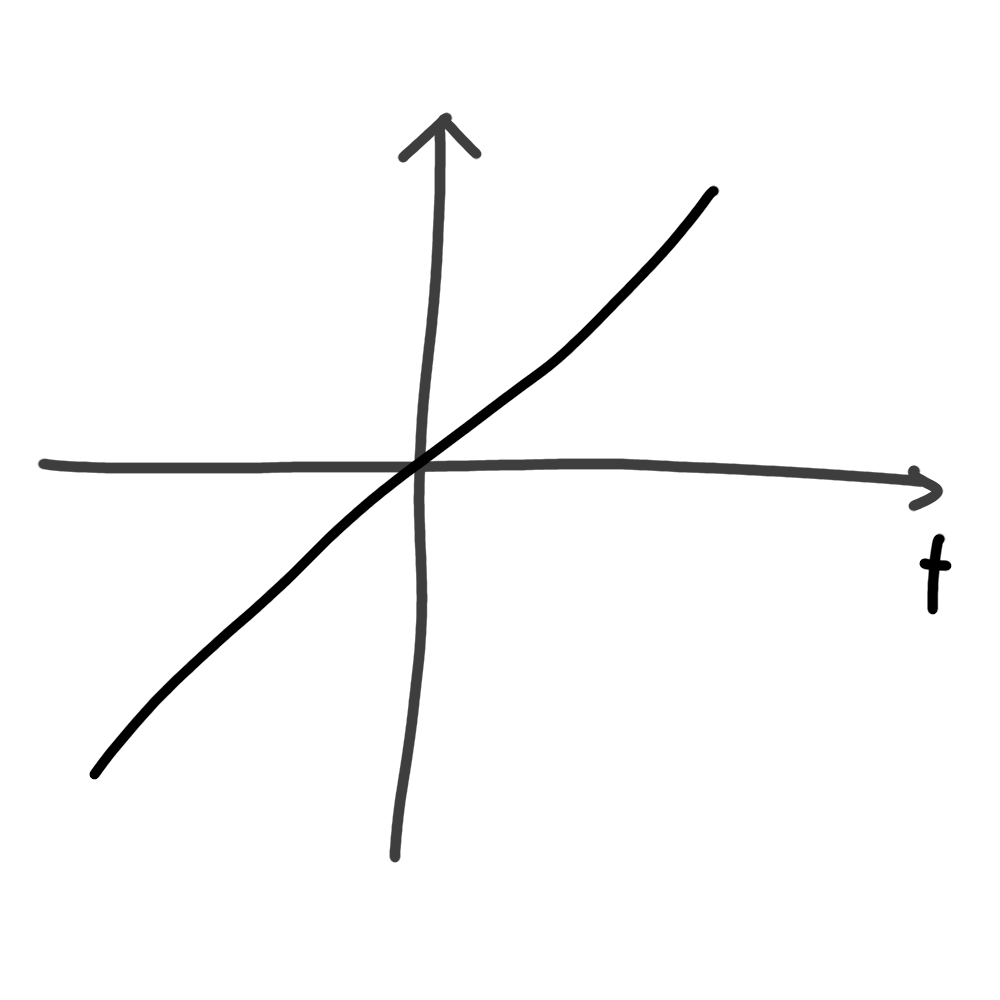
\includegraphics[width=0.3\linewidth]{figures/identity_line}
		\caption{identity line can be parameterized such that $(0, 0)$ is singular.}
		\label{fig:identityline}
	\end{figure}
	
	
	There are curves and points where no parameterisation exists such that the point is regular.	
\end{remark}

\begin{definition}
	$c: I \rightarrow \mathbb{R}^2 \in C^2(I, \mathbb{R}^2)$
	
	The curvature of the curve in the point $c(t)$ is defined as $\kappa(t) = \frac{\det(\dot{c}(t), \ddot{c}(t))}{||\dot{c}(t)||^3}$
\end{definition}

\begin{example}
	\begin{figure}[h!]
		\centering
		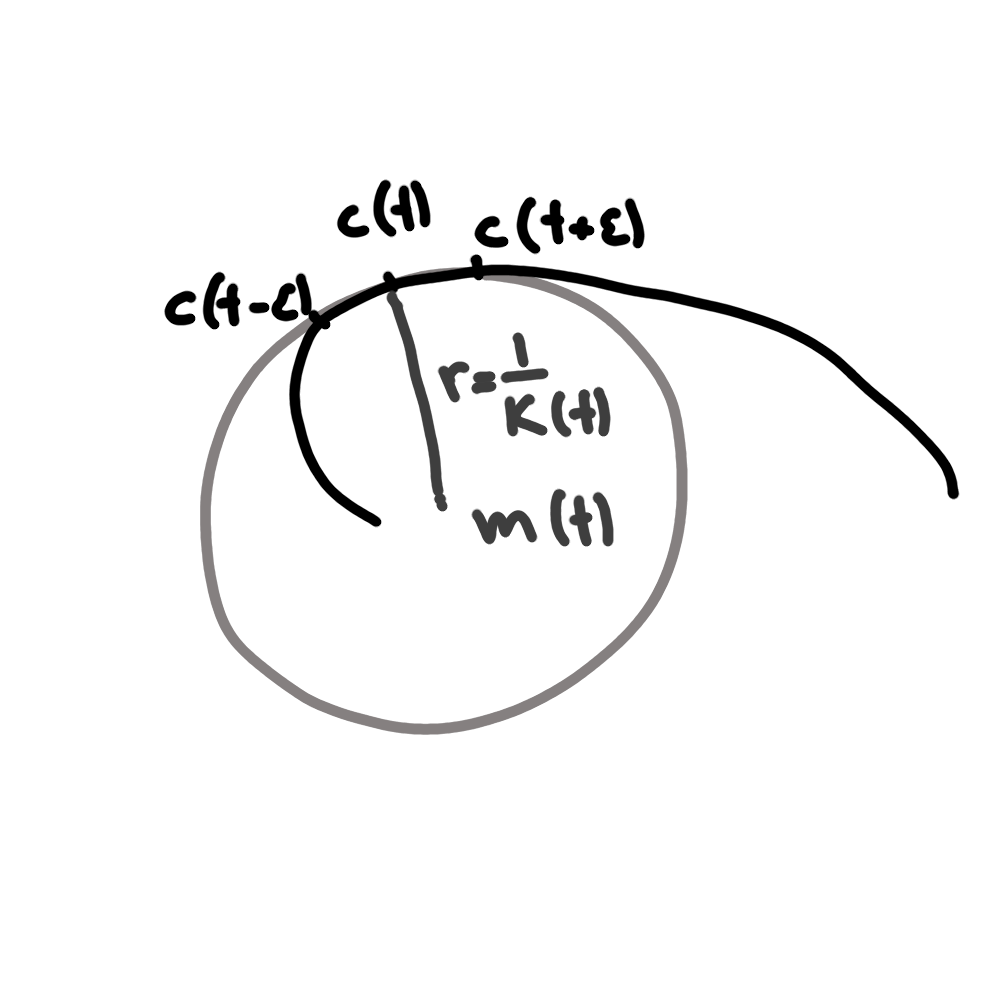
\includegraphics[width=0.3\linewidth]{figures/circle_of_curvature}
		\caption{Circle of curvature}
		\label{fig:circleofcurvature}
	\end{figure}
	
	The circle of curvature has a radius of $\frac{1}{\kappa(t)}$. $m(t)$ is called the center of curvature.
	
	$m(t) = c(t) + \frac{1}{\kappa(t)}n(t)$ where $n(t) = \frac{(-\dot{c_2}(t), \dot{c_1}(t))}{||\dot{c}(t)||}$.
\end{example}

\begin{remark}
	Exercise: compare this definition of curvature with the school version concerning graphs.
\end{remark}

\begin{example}
	For a circle we have $c(t) = (r\cos(t), r\sin(t))^T$, $\dot{c}(t) = (-r\sin(t), r\cos(t))^T$, $\ddot{c}(t) = (-r\cos(t), -r\sin(t))^T$
	
	\begin{align*}
		\kappa(t) = \frac{\det \left(\begin{matrix}
				-r \sin(t) & -r \cos(t) \\
				r \cos(t) & -r \sin(t)
		\end{matrix}\right) }{r^3} = \frac{r^2\sin^2(t) + r^2\cos^2(t)}{r^3} = \frac{r^2}{r^3} = \frac{1}{r}\\
		n(t) = \frac{(-r \cos(t), -r \sin(t))}{r} = (-\cos(t), -\sin(t))
	\end{align*}
	
	\begin{figure}[h!]
		\centering
		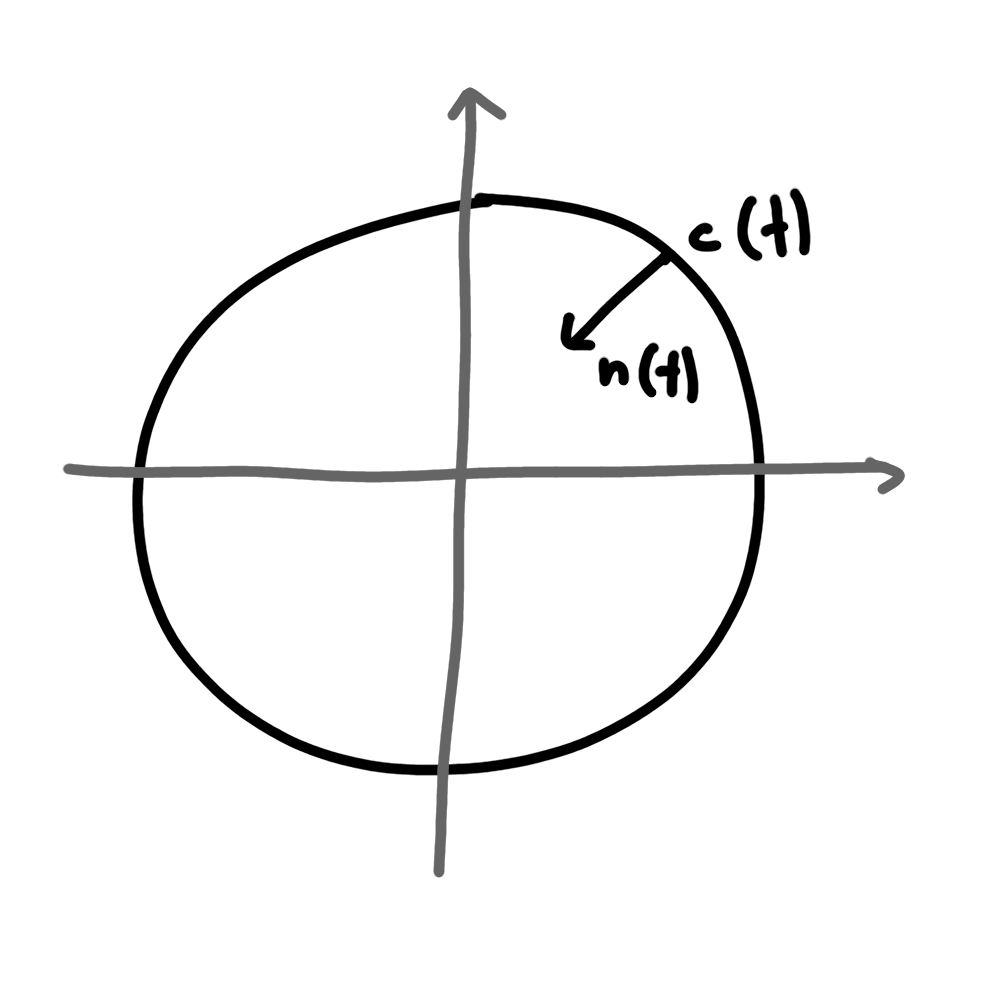
\includegraphics[width=0.3\linewidth]{figures/circle_with_normal_vector}
		\caption{Circle with normal vector}
		\label{fig:circlewithnormalvector}
	\end{figure}
	
\end{example}

\begin{definition}
	A point $c(t)$ with $\dot{\kappa}(t) = 0$ is called a vertex.
\end{definition}

\begin{example}
	An ellipse has four vertices.
	
	\begin{figure}[h!]
		\centering
		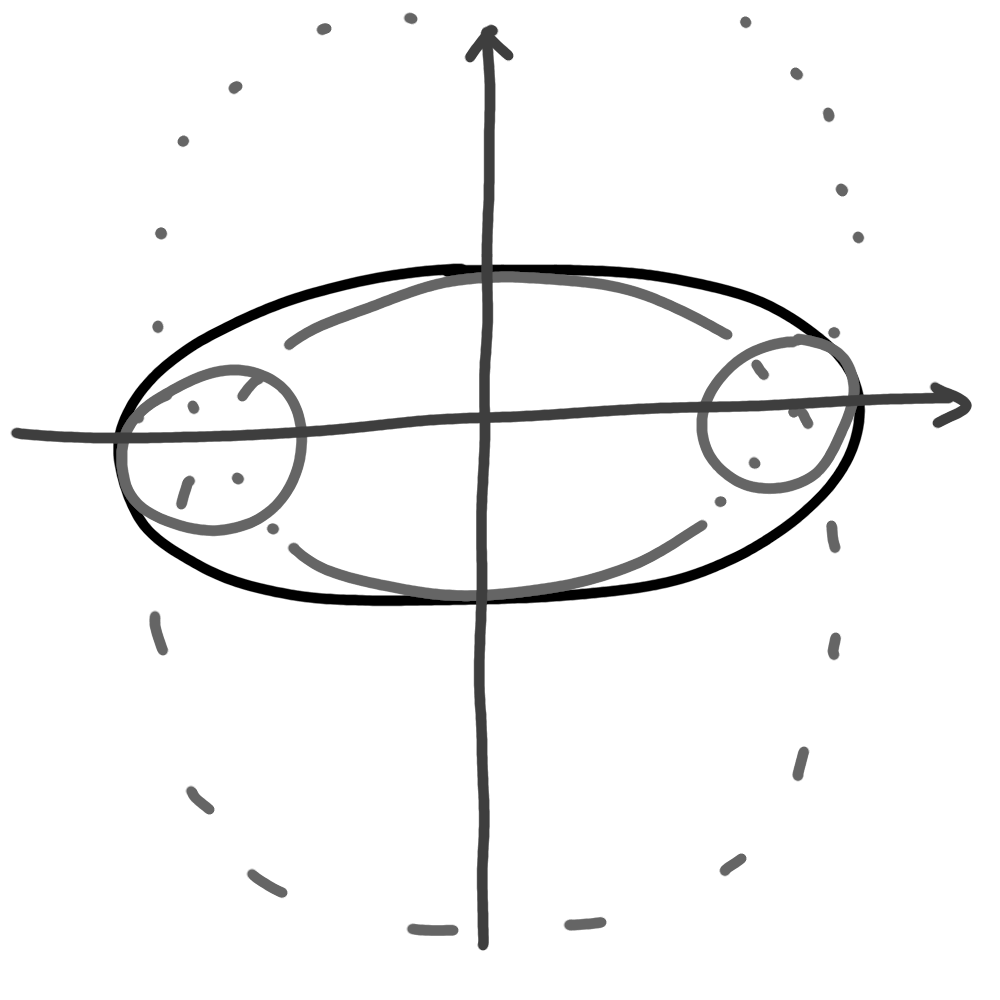
\includegraphics[width=0.3\linewidth]{figures/ellipse}
		\caption{Ellipse and the four vertices.}
		\label{fig:ellipse}
	\end{figure}
	
	
	$(t, \exp t)$ has no vertex.
	
	Klothoids are curves with $\kappa(t) = t$. They are used in road construction and have no vertex.
\end{example}

\begin{definition}
	$c:I \rightarrow \mathbb{R}^3$
	
	$\kappa(t) = \frac{||\dot{c}(t) \times \ddot{c}(t)||}{||\dot{c}(t)||^3}$ is called the curvature of a space curve.
	
	$\tau(t) = \frac{\det (\dot{c}(t), \ddot{c}(t), \dddot{c}(t))}{||\dot{c}(t) \times \ddot{c}(t)||^2}$ is called torsion of a space curve.
\end{definition}

\begin{example}
	For the helix $t \mapsto (\cos(t), \sin(t), pt)$ the torsion depends on $p$.	
\end{example}

\section{Properties of Bezier curves}

\begin{definition}
	$\alpha: \mathbb{R}^n \rightarrow \mathbb{R}^m$ is called \textbf{affine} if $\exists l:\mathbb{R}^n \rightarrow \mathbb{R}^m$...linear $\exists v \in \mathbb{R}^m: \alpha(x) = l(x) + v$.
	
	$\alpha$ is called \textbf{affinity} if $\alpha$ is affine and bijective.
\end{definition}

\begin{example}
	An example of an linear function is shear (Scherung).
	\begin{align*}
		l\left(\begin{matrix} x \\ y \end{matrix}\right) := \left(\begin{matrix} 1 & a \\ 0 & 1 \end{matrix}\right) \left(\begin{matrix} x\\ y \end{matrix}\right)
	\end{align*}
	
	Area is preserved.
	
	\begin{figure}[h!]
		\centering
		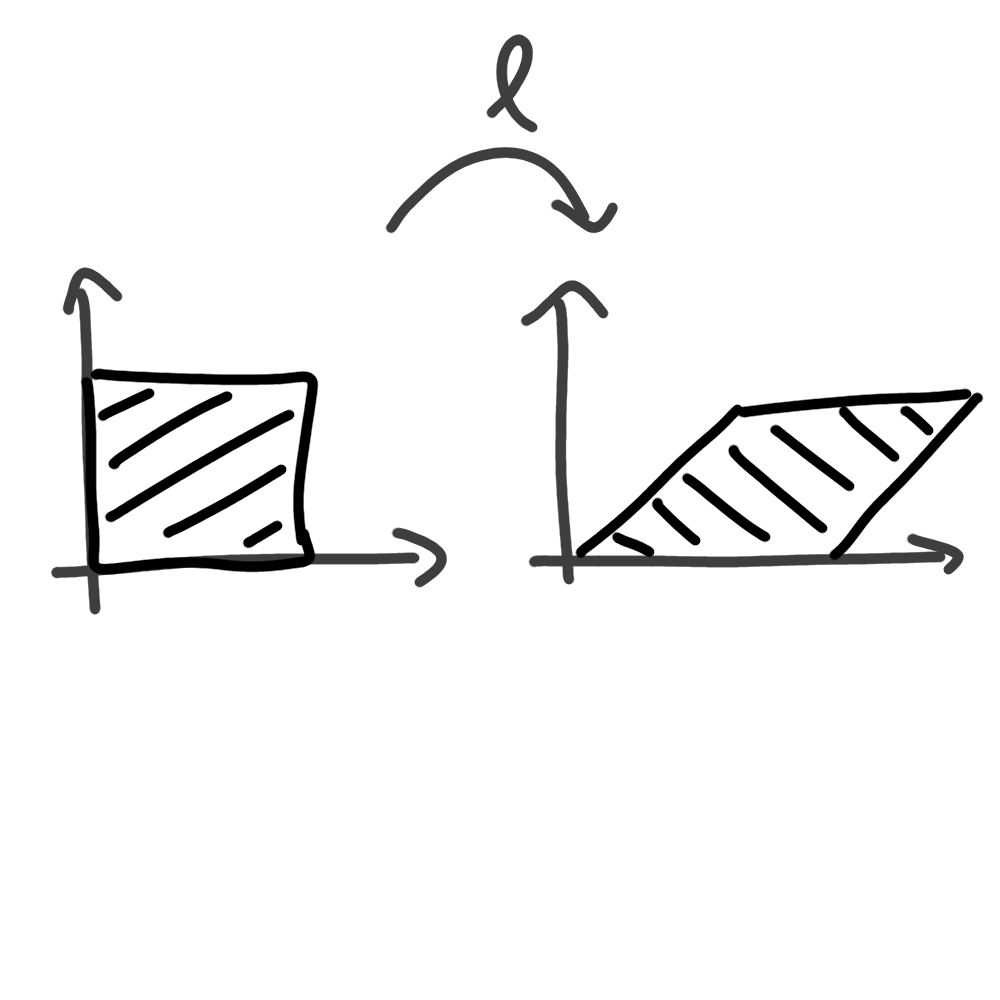
\includegraphics[width=0.3\linewidth]{figures/shear}
		\caption{Shear preserves area}
		\label{fig:shear}
	\end{figure}
\end{example}

\begin{theorem}
	Bezier curves are invariant under affine transformations. 
\end{theorem}

\begin{proof}
	Let $b(t) = \sum_{i=0}^{n} B_i^n(t) b_i$ be a bezier curve and $\alpha(x) = l(x) + v$ where $b_i\in\mathbb{R}^d, l:\mathbb{R}^d\rightarrow\mathbb{R}^m, v \in \mathbb{R}^m$
	\begin{align*}
		\alpha(b(t)) = l(b(t)) + v = l\left(\sum_{i=0}^{n} B_i^n(t) b_i\right) + v = \sum_{i=0}^{n} B_i^n(t) l(b_i) + v =\\
		\sum_{i=0}^{n}B_i^n(t) l(b_i) + \sum_{i=0}^{n}B_i^n(t)v = \sum_{i=0}^{n}B_i^n(t)(l(b_i) + v) = \sum_{i=0}^{n} B_i^n(t) \alpha(b_i)
	\end{align*}
\end{proof}

\begin{figure}[h!]
	\centering
	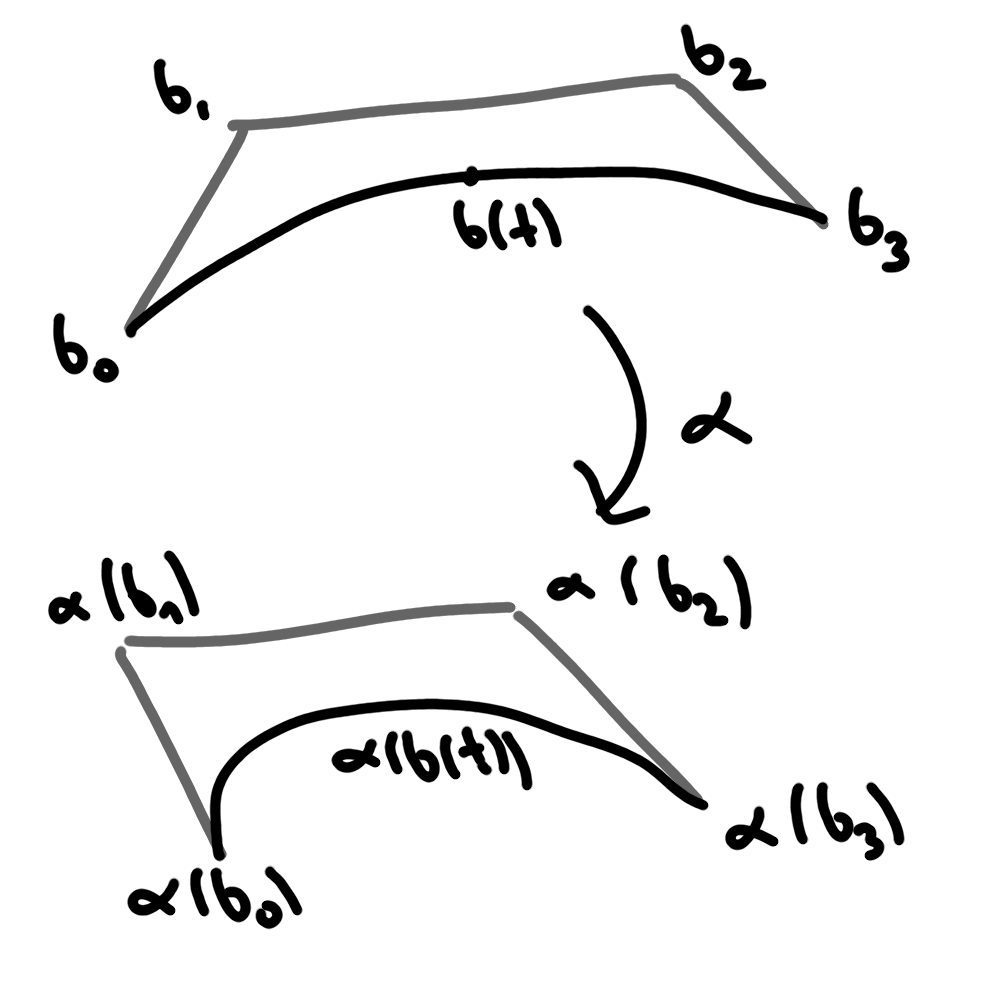
\includegraphics[width=0.3\linewidth]{figures/affine_transformation_bezier}
	\caption{Bezier curve is invariant under affine transformation}
	\label{fig:affine_transformation_bezier}
\end{figure}

\begin{lemma}
	$\sum_{i=0}^{n}B_i^n(t) = 1$
\end{lemma}

\begin{proof}
	Binomial theorem: $(x+y)^n = \sum_{i=0}^{n} \binom{n}{i} x^i y^{n-i}$ for $x=t, y=1-t$ we get
	\begin{align*}
		1 = (t+(1-t))^n = \sum_{i=0}^{n} \binom{n}{i} t^i (1-t)^{n-i} = \sum_{i=0}^{n} B_i^n(t)
	\end{align*}
\end{proof}

\begin{lemma}
	For $t\in[0,1]$ it holds that $B_i^n(t) \geq 0$
\end{lemma}

\begin{proof}
	\begin{align*}
		B_i^n(t) = \underbrace{\binom{n}{i}}_{\geq 0} \underbrace{t^i}_{\geq 0} \underbrace{(1-t)^{n-i}}_{\geq 0} \geq 0
	\end{align*}
\end{proof}

\begin{definition}
	$M \subseteq \mathbb{R}^d$ then $conv(M) := \{\sum_{i=1}^{k} \lambda_i v_i : v_1, ..., v_k \in M, \lambda_1, ..., \lambda_k \geq 0, \sum_{i=1}^{k} \lambda_i = 1, k\in \mathbb{N}\}$ is called the convex hull of M.
	
	$M$ is called convex set, iff $\forall x,y \in M \forall t\in[0,1]: tx+(1-t)y \in M$.
\end{definition}

\begin{example}
	\begin{figure}[h!]
		\centering
		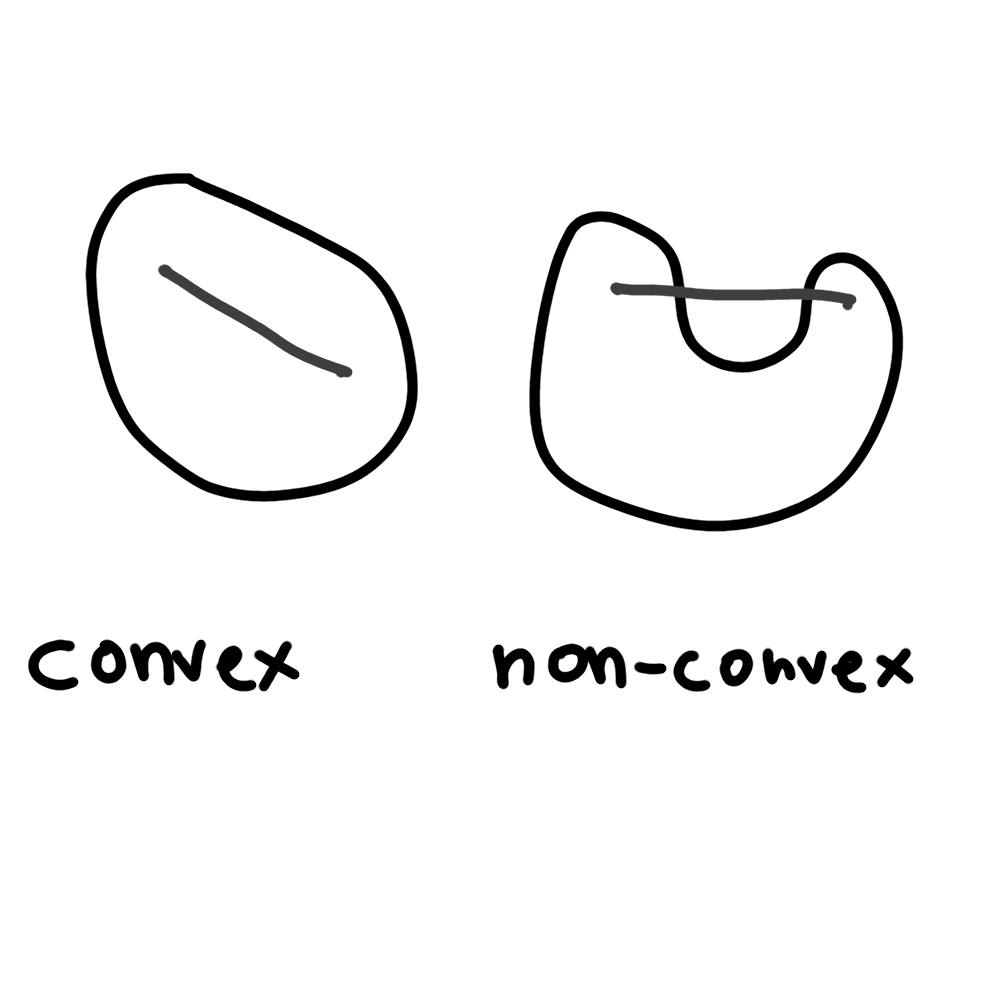
\includegraphics[width=0.3\linewidth]{figures/convex_non_convex}
		\caption{example of convex and non-convex set}
		\label{fig:convex_non_convex}
	\end{figure}
\end{example}

\begin{remark}[Pick theorem]
	For any polygon formed of points in $\mathbb{Z}\times\mathbb{Z}$ it holds that the area can be calculated by $I + R/2 - 1$ where $I$ is the number of points inside the polygon and $R$ is the number of points on the edges of the polygon.
	
	\begin{figure}[h!]
		\centering
		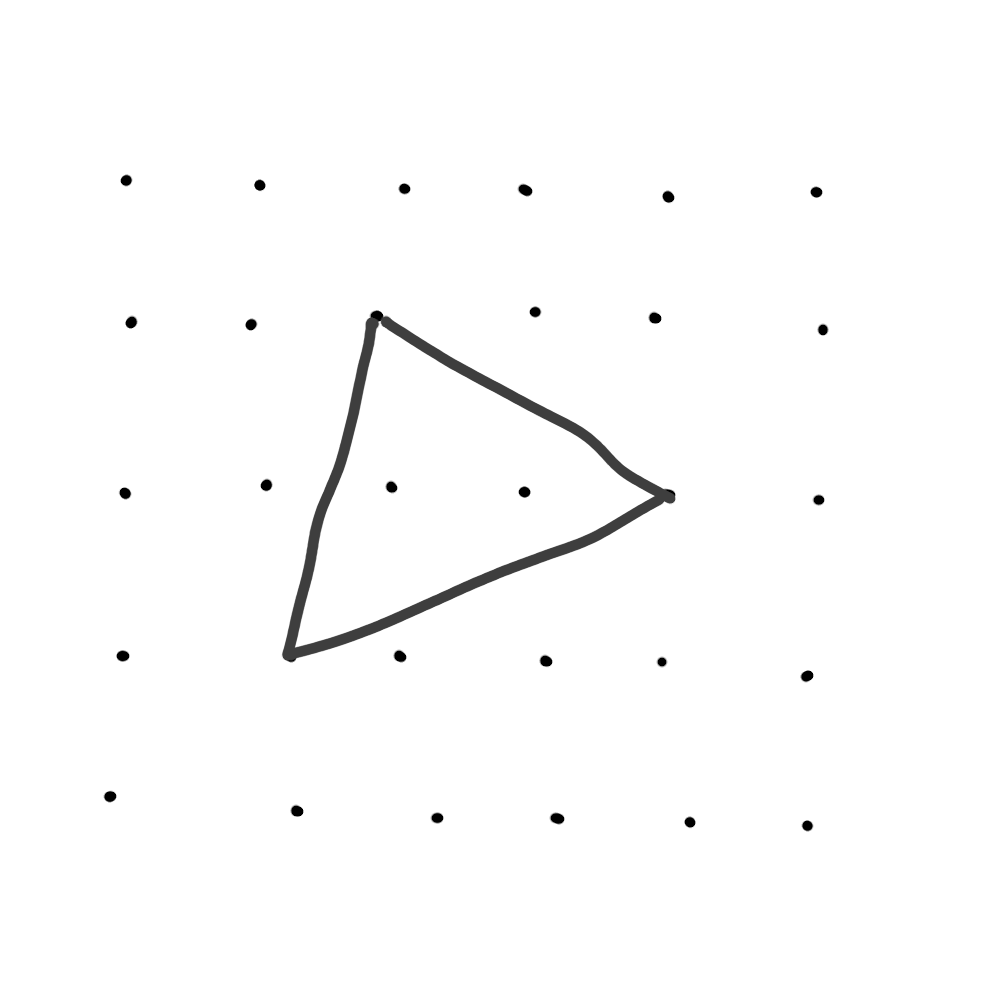
\includegraphics[width=0.3\linewidth]{figures/pick}
		\caption{example picks theorem where $I=2, R=3$ and therefore $A=\frac{5}{2}$}
		\label{fig:pick}
	\end{figure}
\end{remark}

\begin{theorem}
	$\forall t \in [0,1]: b(t) \in conv(\{b_0, b_1, ..., b_n\})$
\end{theorem}

\begin{proof}
	$b(t) = \sum_{i=0}^{n} \underbrace{B_i^n(t)}_{\geq 0} b_i \forall t \in [0,1]$ and $\sum_{i=0}^{n}B_i^n(t) = 1 \forall t \in [0,1]$. Therefore $b(t) \in conv(\{b_0, ..., b_n\})$
\end{proof}

\begin{figure}[h!]
	\centering
	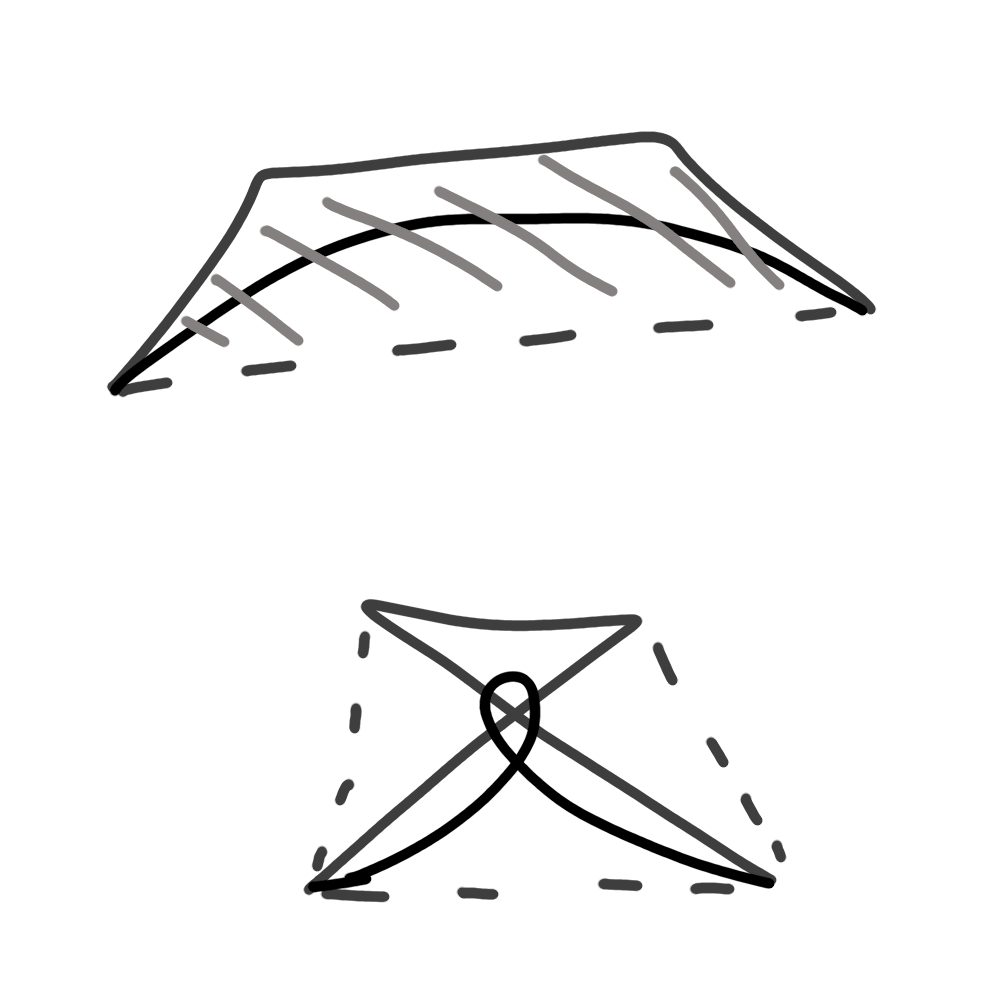
\includegraphics[width=0.3\linewidth]{figures/bezier_curve_in_convex_hull}
	\caption{example of a bezier curve and its convex hull}
	\label{fig:bezier_curve_in_convex_hull}
\end{figure}

\begin{remark}[Montecarlo method for calculating area]
	random points, count how many fall within the area from the total amount of points, estimate volume from that.
	
	\begin{figure}[h!]
		\centering
		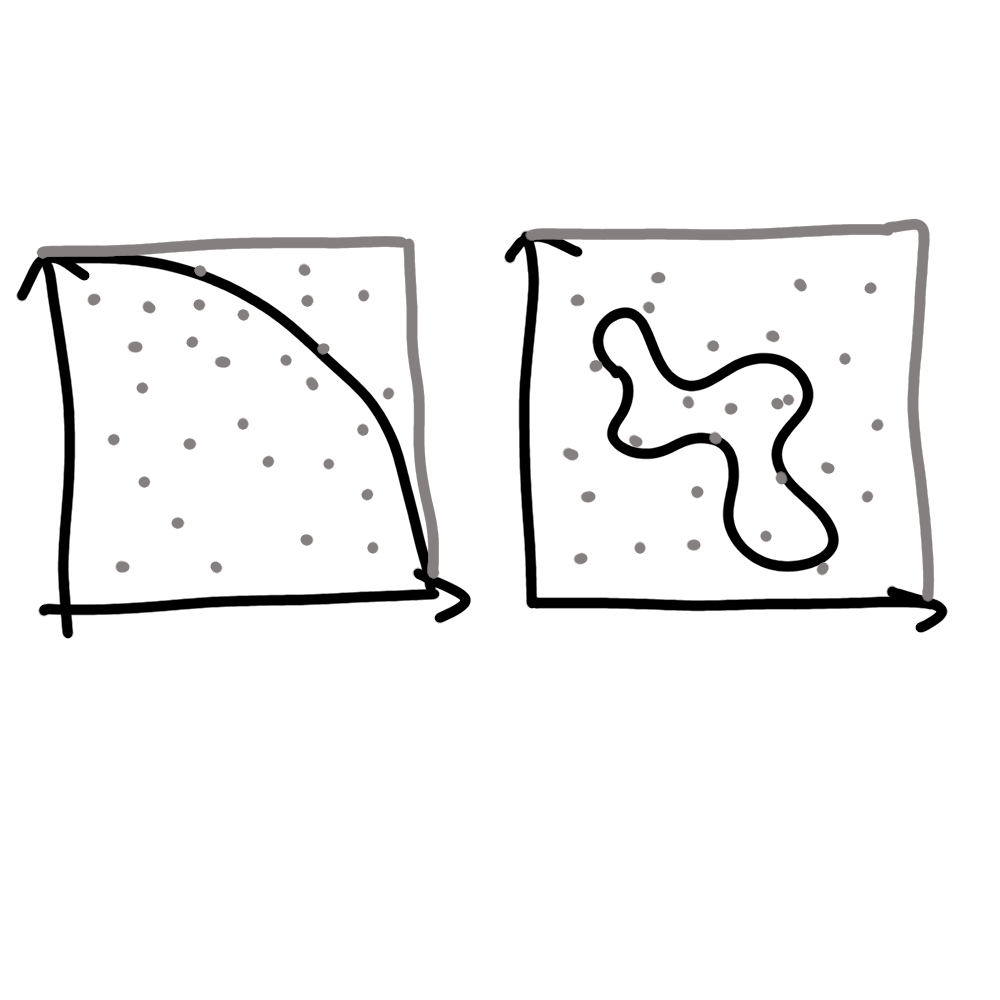
\includegraphics[width=0.3\linewidth]{figures/montecarlo}
		\caption{montecarlo method for a quarter circle and some random shape}
		\label{fig:montecarlo}
	\end{figure}
\end{remark}

\begin{theorem}
	Bezier curves are symmetric, meaning that if $b(t)$ is a bezier curves of $b_0, ..., b_n$ and $\tilde{b}(t)$ is a bezier curve of $b_n, ..., b_0$ then $b(t) = \tilde{b}(1-t)$
\end{theorem}

\begin{proof}
	\begin{align*}
		\tilde{b}(t) = \sum_{i=0}^{n} B_i^n(t) b_{n-i} = \sum_{i=0}^{n} \underbrace{B_i^n(1-t)(1-t)}_{B_i^n(t)}b_{n-i} = \sum_{i=0}^{n} B_{n-i}^n(1-t) b_i = \sum_{i=0}^{n} B_i^n(1-t) b_i = b(1-t)
	\end{align*}
\end{proof}

\begin{lemma}
	$\alpha \in \mathbb{R} \implies B_i^n(\alpha t) = \sum_{j=0}^{n} B_i^j(\alpha) B_j^n(t)$
\end{lemma}

\begin{proof}
	can be done by induction, but is tedious
\end{proof}

\begin{theorem}[Sub-division-property (Unterteilungseigenschaft)]
	Let $b(t)$ be a bezier curve to $b_0, ..., b_n$ and $\alpha \in \mathbb{R}$.
	\begin{align*}
		\tilde{b}(t) := b(\alpha t) && \hat{b}(t) := b((1-\alpha)t + \alpha)
	\end{align*}
	
	Then $\tilde{b}$ is a bezier curve to $b_0^0(\alpha), b_0^1(\alpha), ..., b_0^n(\alpha)$; $\hat{b}$ is a bezier curve to $b_0^n(\alpha), b_1^{n-1}(\alpha), ..., b_n^0(\alpha)$ and ''glued together'' they result in the original bezier curve.
\end{theorem}

\begin{figure}[h!]
	\centering
	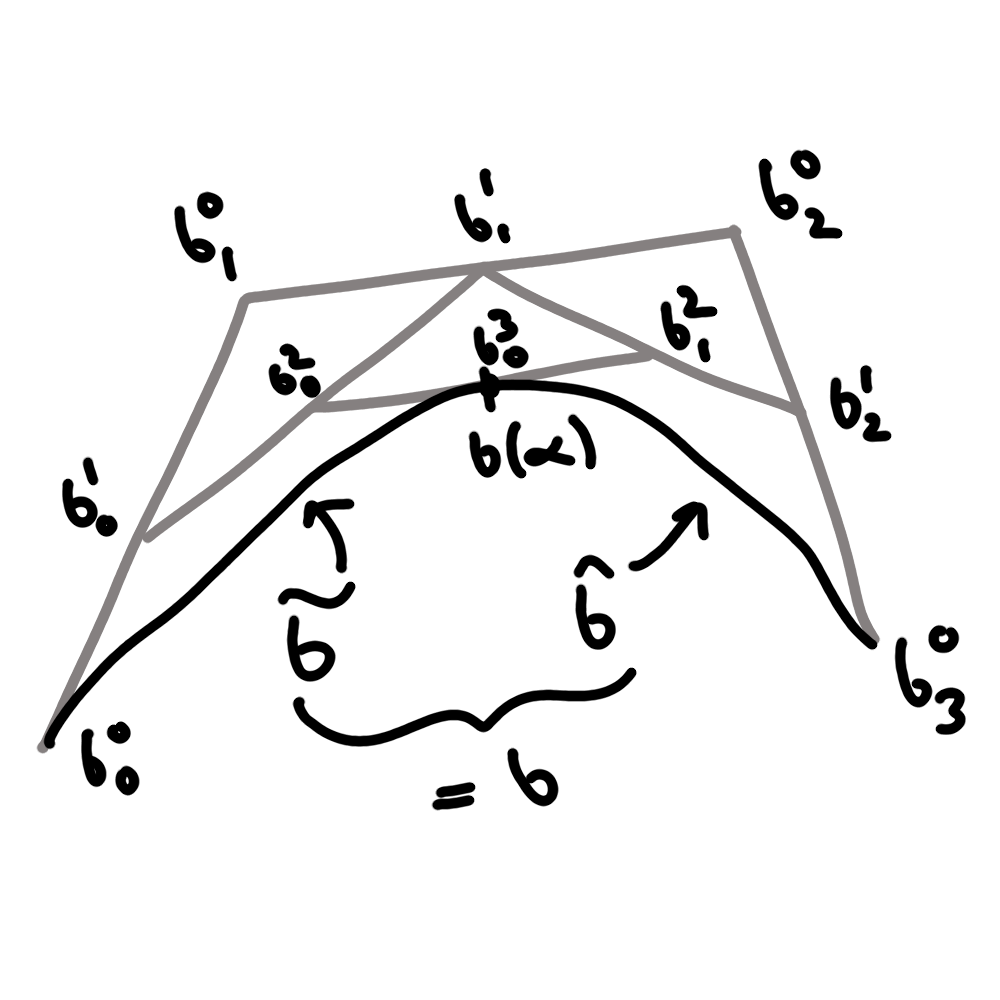
\includegraphics[width=0.3\linewidth]{figures/sub_division}
	\caption{bezier curve $b$ is divided at point $b(\alpha)$ into two bezier curves $\tilde{b}$ and $\hat{b}$}
	\label{fig:sub_division}
\end{figure}

\begin{proof}
	\begin{align*}
		\tilde{b}(t) = b(\alpha t) = \sum_{i=0}^{n} B_i^n(\alpha t) b_i = \sum_{i=0}^{n} \left(\sum_{j=0}^{n}B_i^j(\alpha) B_j^n(t)\right) b_i = \sum_{j=0}^{n} \sum_{i=0}^{n} B_i^j(\alpha) B_j^n(t) b_i =\\
		\sum_{j=0}^{n} B_j^n(t) \underbrace{\sum_{i=0}^{\cancel{n}^j} B_i^j(\alpha) b_i}_{b_0^j(\alpha)} = \sum_{j=0}^{n} B_j^n(t) b_0^j(\alpha)
	\end{align*}
	Where we used $b_i^j(t) = \sum_{l=0}^{j} B_l^j(t) b_{i+l}$, which we already showed.
	
	$\hat{b}$ is analogous.
\end{proof}

\begin{definition}
	The polynomial ring is defined as $\Pi_n := \{f \in \mathbb{R}[t] : deg(f) \leq n\}$, which is a vector space.
\end{definition}

\begin{theorem}
	$\{B_0^n(t), ..., B_n^n(t)\}$ is a basis of $\Pi_n$.
\end{theorem}

\begin{proof}
	$\forall i: B_i^n(t) \in \Pi_n$ therefore $span(B_0^n(t), ..., B_n^n(t)) \subseteq \Pi_n$.
	
	We know that $dim(\Pi_n) = n+1$ as $\{1, t, t^2, ..., t^n\}$ is a basis.
	
	Let $k \leq n$.
	
	\begin{align*}
		1 = \sum_{i=0}^{n-k} B_i^{n-k}(t) = \sum_{i=k}^{n} B_{i-k}^{n-k}(t) = \sum_{i=k}^{n} \binom{n-k}{i-k} t^{i-k} (1-t)^{n-i}\\
		\implies \binom{n}{k} t^k = \sum_{i=k}^{n} \binom{n}{k} \binom{n-k}{i-k} t^i (1-t)^{n-i} = \sum_{i=k}^{n} \binom{n}{i} \binom{i}{k} t^i (1-t)^{n-i} = \sum_{i=k}^{n} \binom{i}{k} B_i^n(t)\\
		\implies t^k \in span(B_0^n(t), ..., B_n^n(t)) \implies \Pi_n \subseteq span(B_0^n(t), ..., B_n^n(t))
	\end{align*}
\end{proof}

\begin{corollary}
	Every polynomial curve is a bezier curve.
\end{corollary}

\begin{theorem}[corner-cutting (Eckenabschneiden)]
	Define the sequence $P_n$ by this (recursive) definition $P_0 := (b_0^0, b_0^1, ..., b_0^n)$, $P_1 := (b_0^0, b_0^1, ..., b_0^n, b_1^{n-1}, b_2^{n-2}, ..., b_n^0)$, ..., $P_n$ consists of the points we get by sub-dividing the bezier curve (with $t=\frac{1}{2}$).
	
	Then this sequence ''converges'' to the bezier curve
\end{theorem}

\begin{proof}
	$d := \max_{0 \leq i \leq n} ||b_i - b_{i+1}||$ ... maximum length of edges of control polygon
	
	\begin{figure}[h!]
		\centering
		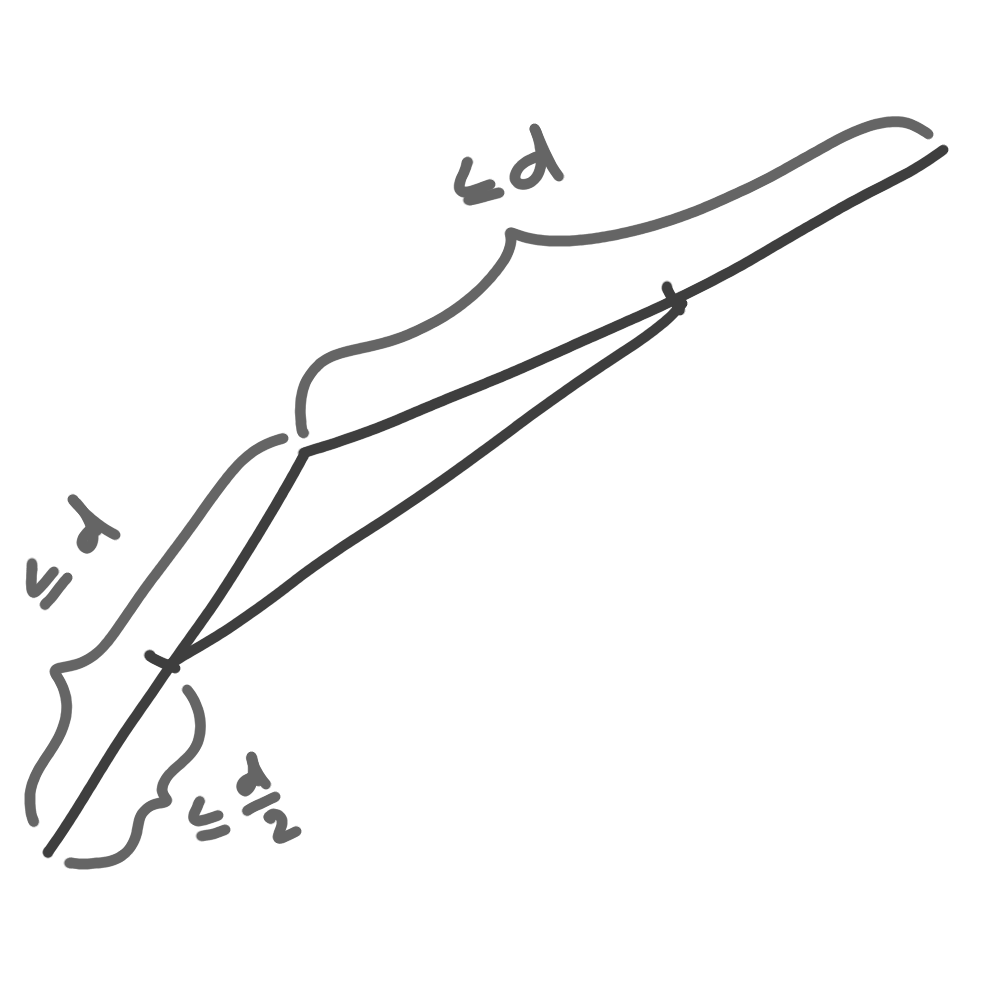
\includegraphics[width=0.3\linewidth]{figures/corner_cutting}
		\caption{the new edges are at most $\frac{d}{2}$ long}
		\label{fig:corner_cutting}
	\end{figure}
	
	From the image we can deduce that the maximum length of the edges of the new control polygon is at most $\frac{d}{2}$. With induction we get that the control polygon of $P_n$ has the maximum edge length of $\frac{d}{2^n}$.
	
	How far are the points of the control polygon from the bezier curve $b$? $||P_k(i) - b|| \leq (n-1) \frac{d}{2^k} \rightarrow 0$ for $k \rightarrow \infty$.
\end{proof}

\begin{remark}
	Not only does the sequence from the theorem converge pointwise, but it holds that $P_n \rightarrow b$.
\end{remark}

\begin{remark}
	Disadvantages of bezier curves are: unintuitive, local changes are not possible as every change in a control point changes the entire curve, points can be far away from the curve.
\end{remark}

\section{B-Spline-Curves}

\begin{definition}
	B-Spline curves are compositions of bezier curves.
\end{definition}

\begin{example}
	\begin{figure}[h!]
		\centering
		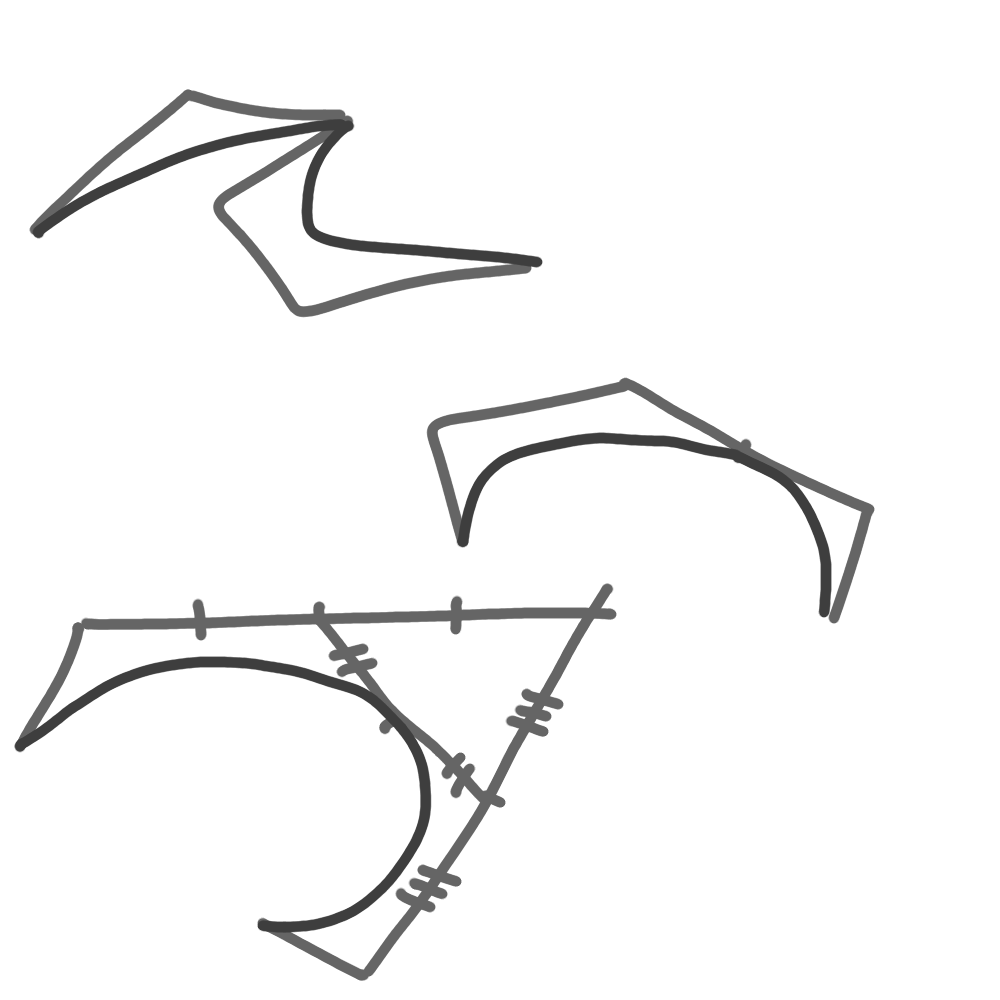
\includegraphics[width=0.3\linewidth]{figures/continous_b_spline}
		\caption{continuous, tangential continuous and curvature continuous composition}
		\label{fig:continous_b_spline}
	\end{figure}
\end{example}

\begin{definition}[B-Spline-Curves]
	$m\in \mathbb{N}$ is the number of control points, $n \in \mathbb{N}$ is the degree of the b spline curve, $T=(t_0, t_1, ..., t_{m+n+1})$ where $t_i \in \mathbb{R}$, $t_i \leq t_{i+1}$ and $t_i < t_{i+n+1}$ is called knot vector (Knotenvektor).
	
	\begin{align*}
		\alpha_i^r(t) := \begin{cases}
								\frac{t - t_i}{t_{i+r} - t_i} & t_{i+r} - t_i \neq 0\\
								0 & \text{else}
							\end{cases}
	\end{align*}
	\begin{align*}
		N_i^0(t) := \begin{cases}
						1 & t \in [t_i, t_{i+1})\\
						0 & \text{else}
					\end{cases} &&
		N_i^r(t) := \alpha_i^r(t) N_i^{r-1}(t) + (1-\alpha_{i+1}^r(t))N_{i+1}^{r-1}(t)
	\end{align*}
	
	$N_i^r:\mathbb{R} \rightarrow \mathbb{R}$ are called b-spline basis functions (B-Spline-Basisfunktionen) and are piece-wise polynomial curves.
\end{definition}

\begin{theorem}
	Every b-spline curve $s(t)$ can be expressed in the form $s(t) = \sum_{i=0}^{m} N_i^n(t) c_i$ where $c_0, ..., c_m \in \mathbb{R}^d$ are the control points and $n$ is the degree of the b-spline curve.
\end{theorem}

\begin{proof}
	without proof
\end{proof}

\begin{example}
	\begin{figure}[h!]
		\centering
		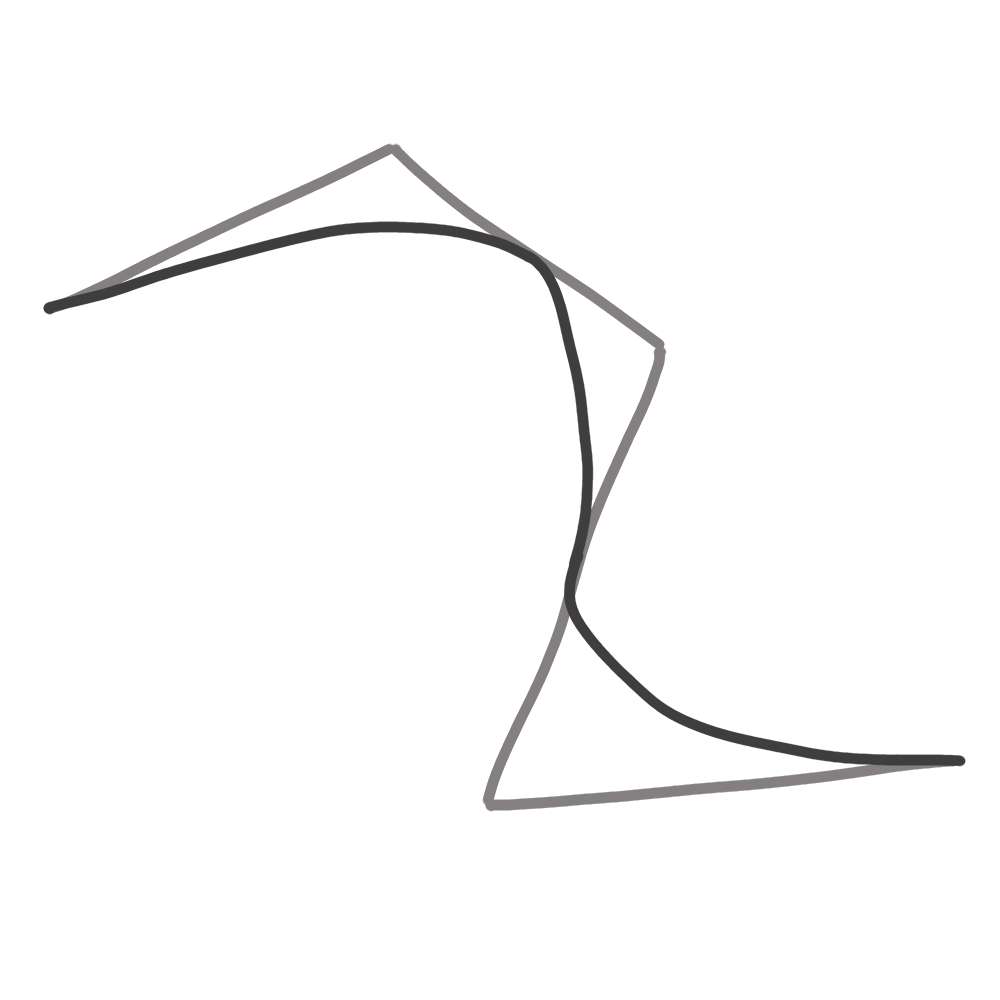
\includegraphics[width=0.3\linewidth]{figures/quadratic_b_spline}
		\caption{from this set of control points there are different possible quadratic b-spline curves (depending on the chosen knot vector).}
		\label{fig:quadratic_b_spline}
	\end{figure} 
\end{example}

\begin{remark}
	Typically a knot vector of a similar form as $T = (0, 0, 0, 0, 1, 2, 3, 4, 5, 5, 5, 5)$ is chosen. $0$ often repeated, then counting up, then as many numbers of the same value as $0$ in the start.
\end{remark}

\begin{example}
	\begin{figure}[h!]
		\centering
		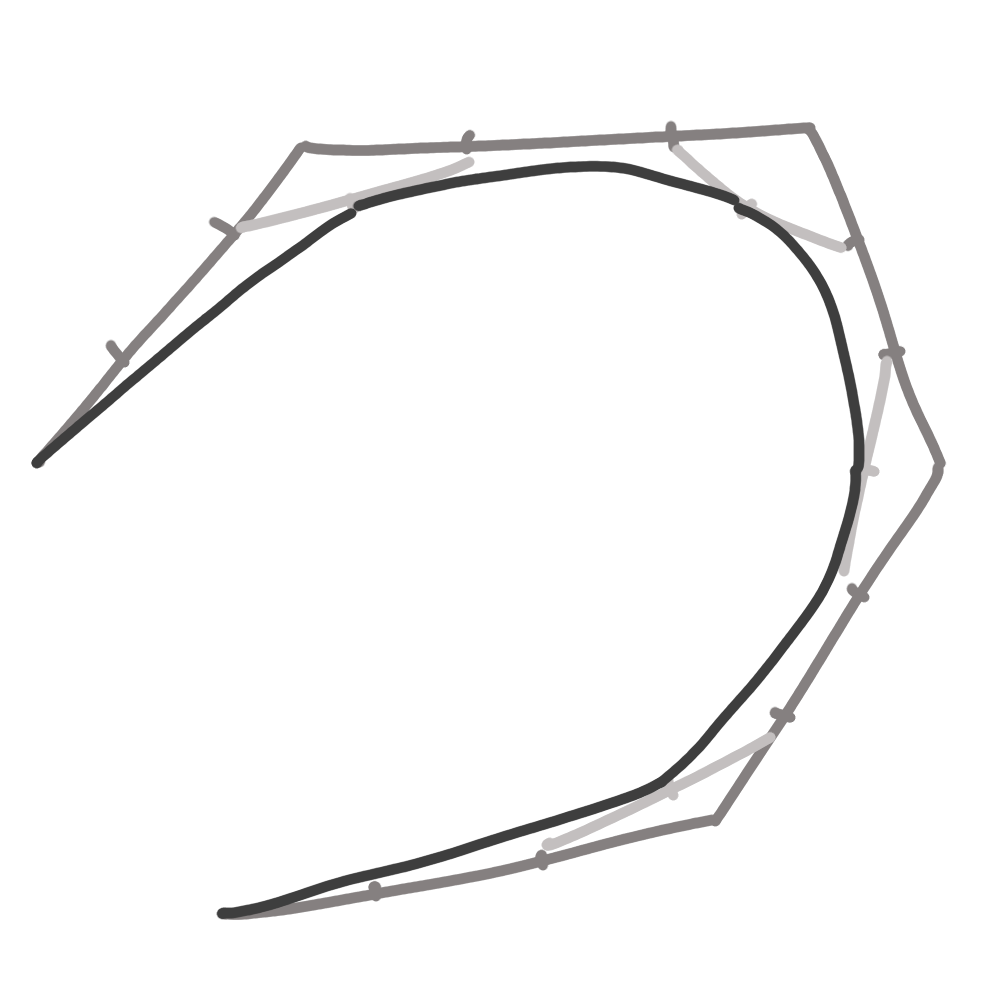
\includegraphics[width=0.3\linewidth]{figures/cubic_b_spline}
		\caption{cubic b-spline curve}
		\label{fig:cubic_b_spline}
	\end{figure} 
	
	Every line segment in the control polygon is cut into thirds.
\end{example}

\begin{example}
	closed b-spline curves
	\begin{figure}[h!]
		\centering
		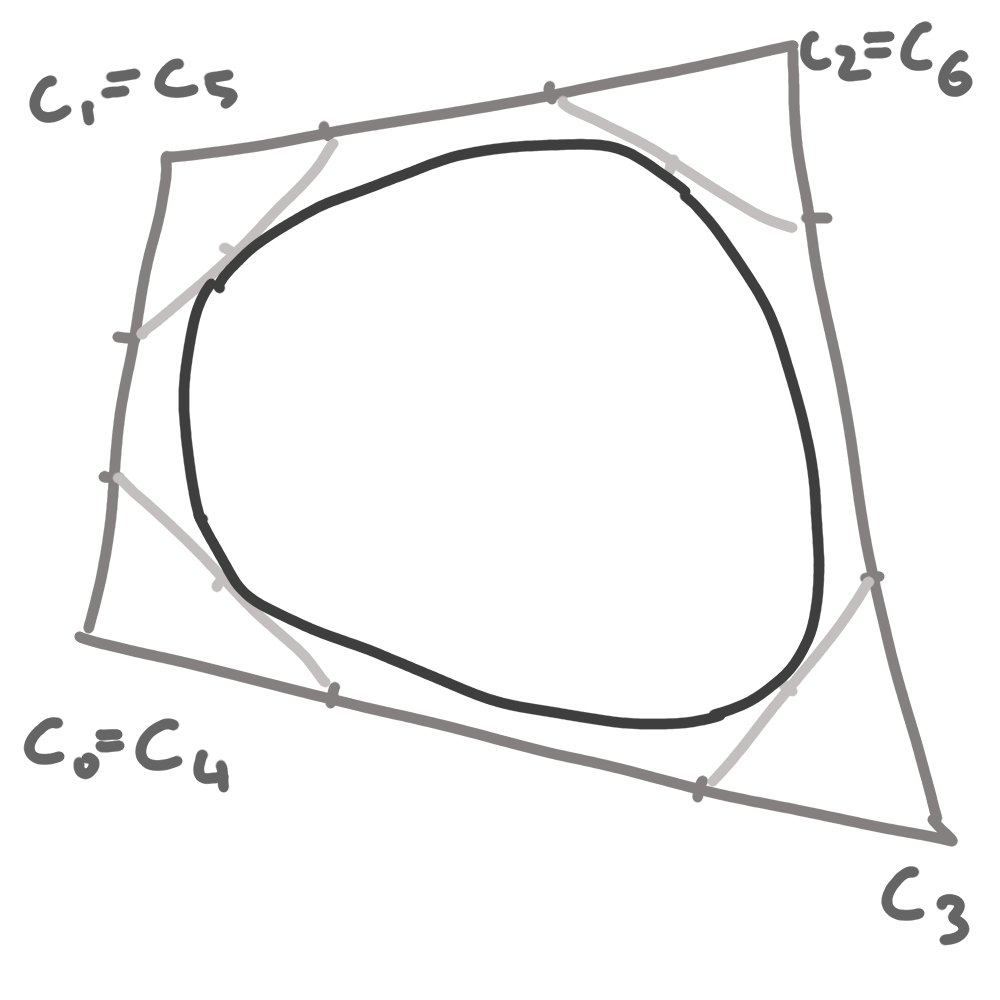
\includegraphics[width=0.3\linewidth]{figures/closed_b_spline}
		\caption{curvature continuous, closed b-spline curve.}
		\label{fig:closed_b_spline}
	\end{figure} 
\end{example}

\begin{remark}
	B-spline curves of degree $n$ with $n+1$ control points ($\implies m=n$) are bezier curves.
\end{remark}

\section{NURBS-Curve}

\begin{remark}
	Non-Uniform-Rational-B-Spline-Curve
\end{remark}

\begin{figure}[h!]
	\centering
	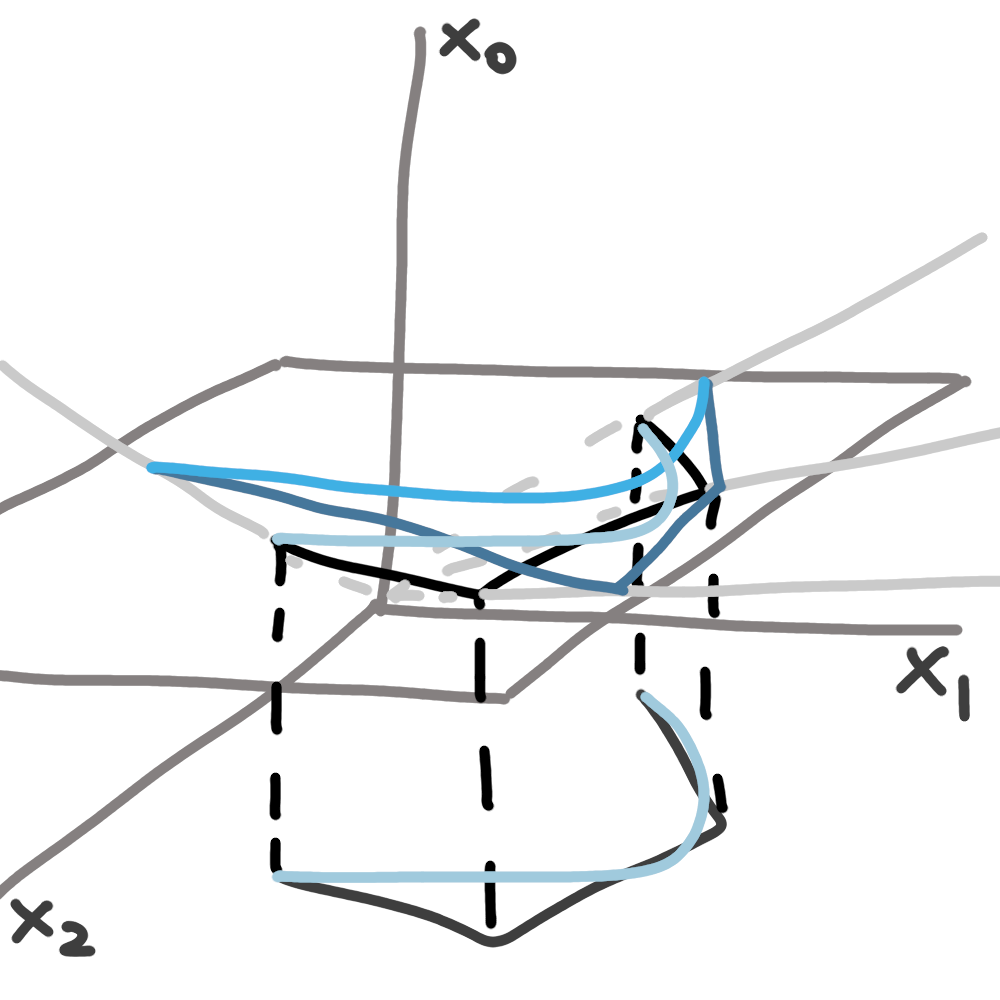
\includegraphics[width=0.3\linewidth]{figures/nurbs_construction}
	\caption{construction of a nurbs curve}
	\label{fig:nurbs_construction}
\end{figure}

\begin{lemma}[Construction of a NURBS curve]
	\begin{enumerate}
		\item given are control points $c_0, ..., c_m \in \mathbb{R}^d$
		\item $d_i := (1, c_i) \in \mathbb{R}^{d+1}$ (this is called transforming into homogeneous coordinates (homogenisieren))
		\item choose weights $w_i > 0$. $e_i := w_i d_i \in \mathbb{R}^{d+1}$
		\item calculate b-spline curve with control points $e_i$
		\begin{align*}
			s(t) := \sum_{i=0}^{m} N_i^n(t) e_i = \sum_{i=0}^{m} N_i^n(t) w_i (1,c_i) = \left(\sum_{i=0}^{m} N_i^n(t) w_i, \sum_{i=0}^{m} N_i^n(t) w_i c_i\right)
		\end{align*}
		\item project $s(t)$ back into the $(1 \times \mathbb{R}^d)$ plane
		\begin{align*}
			\tilde{x}(t) = pr(s(t)) = \left(1, \frac{\sum_{i=0}^{m} N_i^n(t) w_i c_i}{\sum_{i=0}^{m} N_i^n(t) w_i}\right)
		\end{align*}
		\item dehomogenate
		\begin{align*}
			x(t) := pr_{\mathbb{R}^d}(\tilde{x}) = \frac{\sum_{i=0}^{m} N_i^n(t) w_i c_i}{\sum_{i=0}^{m} N_i^n(t) w_i}
		\end{align*}
	\end{enumerate}
	
	$x(t)$ is called the NURBS curve with weights $w_0, .., w_m$
\end{lemma}

\begin{remark}
	In the special case $w_i = w \in \mathbb{R}^+$ the NURBS curve is a B-spline curve.
\end{remark}

\begin{remark}
	\begin{align*}
		\sum_{i=0}^{m} N_i^n(t) = 1 && N_i^n(t) \geq 0
	\end{align*}
\end{remark}

\begin{remark}
	The bigger $w_i$ is the more the curve is attracted towards $c_i$.
\end{remark}

\begin{remark}
	NURBS and B-splines are invariant under affine transformations.
\end{remark}

\begin{example}
	NURBS-curve over a quadratic bezier curve.
	
	\begin{align*}
		b(t) = (1-t)^2b_0 + 2(1-t)tb_1 + t^2b_2\\
		x(t) = \frac{(1-t)^2w_0b_0 + 2(1-t)tw_1b_1 + t^2w_2b_2}{(1-t)^2w_0 + 2(1-t)tw_1 + t^2w_2}
	\end{align*}
	
	$x(t)$ is a central projection of a parabola, and therefore a conic section (Kegelschnitt).
\end{example}

\begin{example}
	$w_0 = w_1 = w_2$ then $x(t) = b(t)$ which is a parabola.
\end{example}

\begin{example}
	$w_0 = w_2 = 1$, $w:=w_1$ How do we have to choose $w$ in order for $x(t)$ to be a different conic section from a parabola?
	
	$x(t)$ is a $\begin{cases}
		\text{ellipse}\\
		\text{parabola}\\
		\text{hyperbola}
	\end{cases}$ if $x(t)$ has $\begin{cases}
	0\\
	1\\
	2
	\end{cases}$ points at infinity (Fernpunkt).
	
	Therefore we investigate how often the denominator is $0$. 
	
	\begin{align*}
		(1-t)^2 + 2(1-t)tw + t^2 = 1 - 2t + t^2 + 2tw - 2t^2w + t^2 = (2-2w)t^2 + (-2+2w)t + 1\\
		t_{1,2} = \frac{2-2w \pm \sqrt{(2-2w)^2 - 4(2-2w)}}{2(2-2w)}\\
		(2-2w)^2 - 4(2-2w) = 4 - 8w + 4w^2 - 8 + 8w = 4w^2 - 4 = 4(w^2 - 1)
	\end{align*}
	
	If $w=1$ we have already seen that the result is a parabola. Otherwise we do not divide by $0$. We are interested in what is under the square root.
	
	As $4(w^2-1) = 0 \iff w=1$ we have $\begin{cases}0\\ 1\\ 2\end{cases}$ real roots if $4(w^2-1) \begin{cases}<0\\ =0\\ >0\end{cases}$.
\end{example}

\begin{theorem}
	$x(t)$ is a $\begin{cases}
		\text{ellipse}\\
		\text{parabola}\\
		\text{hyperbola}
	\end{cases}$ if $\begin{cases}w<1\\ w=1\\ w>1\end{cases}$.
\end{theorem}

\begin{figure}[h!]
	\centering
	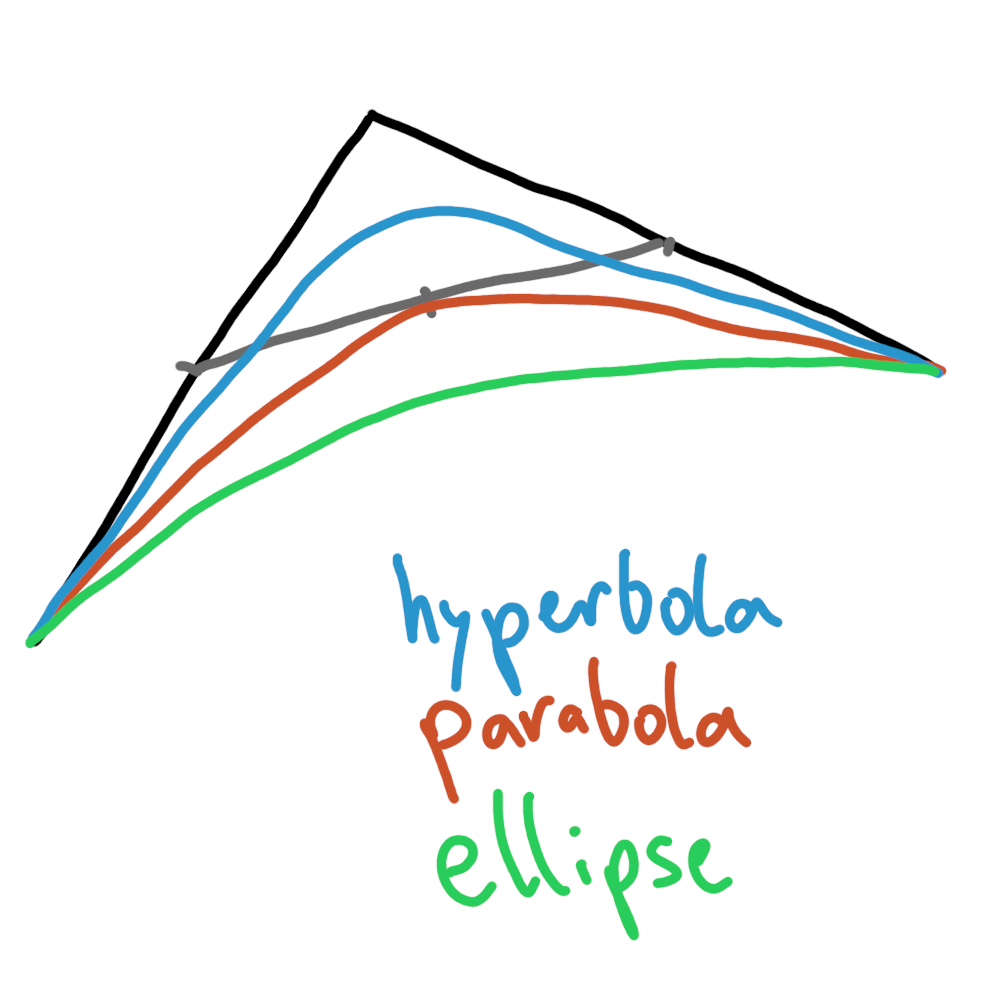
\includegraphics[width=0.3\linewidth]{figures/nurbs_par_hyp_ellip}
	\caption{NURBS curve for the different values of $w$}
	\label{fig:nurbs_par_hyp_ellip}
\end{figure}

\begin{example}
	Is it possible to make a circle?
	
	Obviously the distance between $b_1$ and the two points $b_0$ and $b_2$ must be equal.
	
	\begin{figure}[h!]
		\centering
		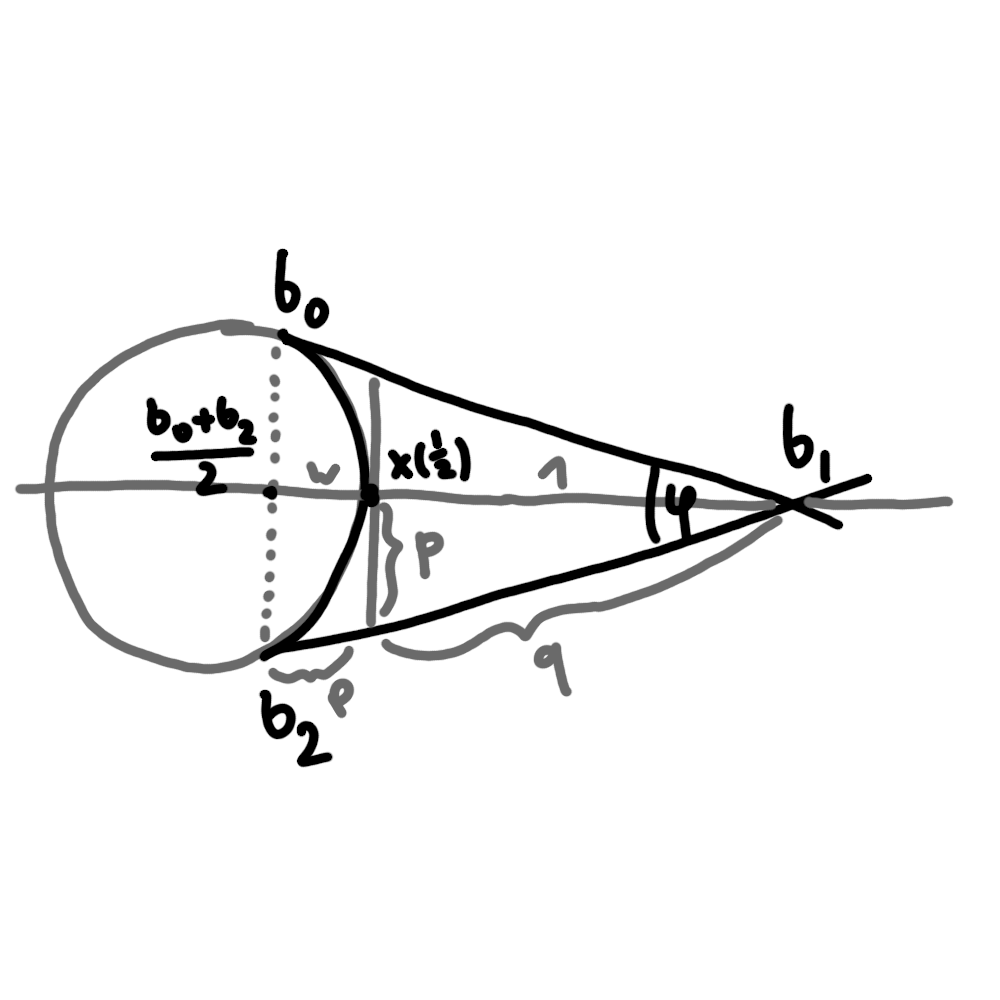
\includegraphics[width=0.3\linewidth]{figures/nurbs_circle}
		\caption{depection of conditions in order for $x(t)$ to be a circle}
		\label{fig:nurbs_circle}
	\end{figure}
	
	A necessary condition is therefore that $b_0, b_1, b_2$ form an isosceles (gleichschenkelig) triangle.
	
	
	\begin{align*}
		x(\frac{1}{2}) = \frac{(1-\frac{1}{2})^2b_0 + 2(1-\frac{1}{2})\frac{1}{2}wb_1 + (\frac{1}{2})^2b_2}{(1-\frac{1}{2})^2 + 2(1-\frac{1}{2})\frac{1}{2}w + (\frac{1}{2})^2} = \frac{\frac{1}{4}b_0 + \frac{1}{2}b_1 + \frac{1}{4}b_2}{\frac{1}{4} + \frac{1}{2}w + \frac{1}{4}} = \frac{b_0 + 2wb_1 + b_2}{2+2w} =\\
		\frac{1}{2+2w}(b_0 + b_2 + 2wb_1) = \frac{1}{1+w}(\frac{b_0+b_2}{2} +wb_1) = \frac{1}{1+w} \frac{b_0 + b_2}{2} + \frac{w}{1+w} b_1
	\end{align*}
	which is a affine combination of $\frac{b_0 + b_2}{2}$ and $b_1$.
	
	\begin{figure}[h!]
		\centering
		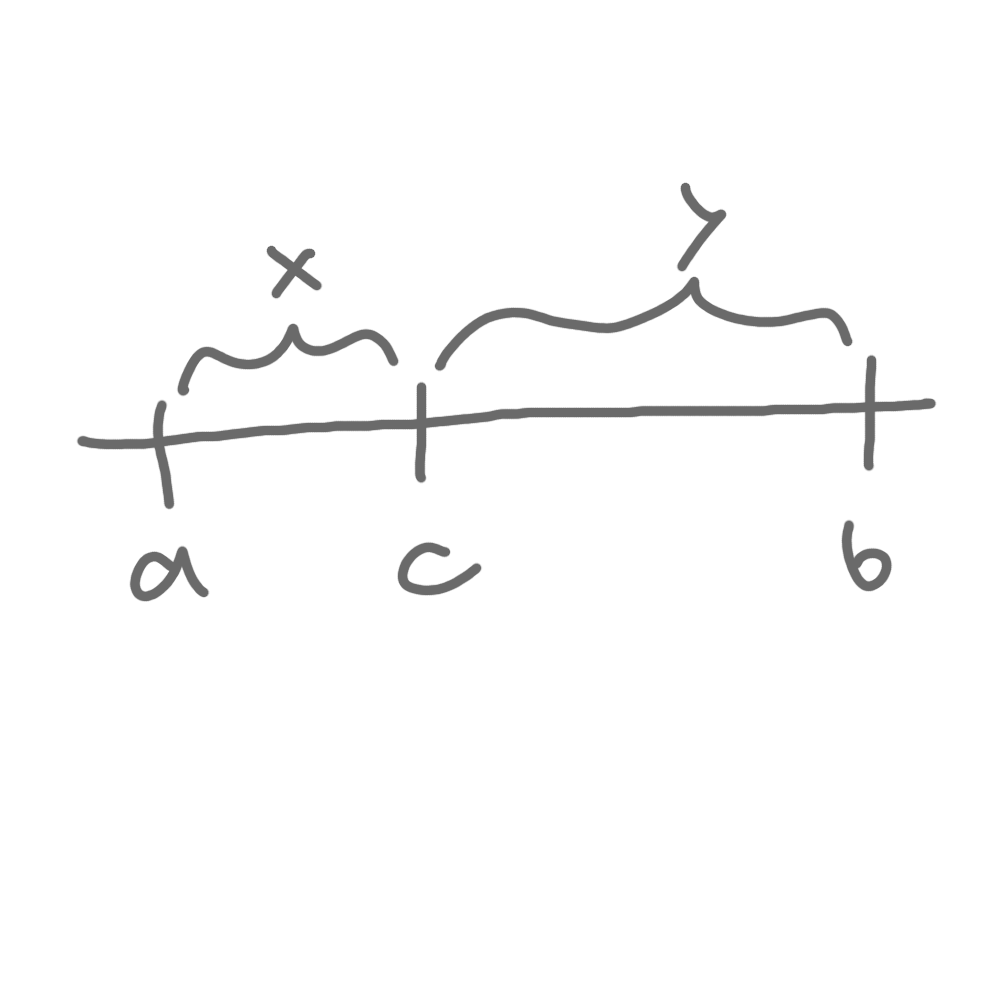
\includegraphics[width=0.3\linewidth]{figures/nurbs_ratio}
		\caption{ratio between distances between points on a line}
		\label{fig:nurbs_ratio}
	\end{figure}
	
	\begin{align*}
		c = (1-\lambda)a + \lambda b\\
		\frac{x}{y} = \frac{c-1}{b-c} = \frac{(1-\lambda)a + \lambda b - a}{b - (1-\lambda) a - \lambda b} = \frac{\lambda(b-a)}{(1-\lambda)(b-a)} = \frac{\lambda}{1-\lambda}
	\end{align*}
	
	For $(1-\lambda)a + \lambda b = (\frac{1}{1-w})\frac{b_0+b_2}{2} + \frac{w}{1+w}b_1$ we get $\frac{x}{y} = \frac{\lambda}{1-\lambda} = \frac{\frac{w}{1+w}}{\frac{1}{1+w}} = w$.
	
	With the intercept theorem (Strahlensatz) and law of sines (trigonometrischer Satz) we get $\sin(\frac{\phi}{2}) = \frac{p}{q} = w$.
	
	$\implies w = \sin(\frac{\phi}{2})$.
\end{example}

\begin{theorem}
	$x(t)$ is a circle, if $b_0, b_1, b_2$ is an isosceles triangle and $w_0=w_2=1$, $w_1 = \sin(\frac{\phi}{2})$ where $\phi = \angle (b_0-b_1, b_2, b_1)$.
\end{theorem}

\begin{remark}
	How can we calculate the angle?
	
	\begin{align*}
		\cos(\phi) = \frac{<b_0-b_1, b_2-b_1>}{||b_0-b_1||\cdot ||b_2-b_1||}
	\end{align*}
	
	With further calculations we get
	\begin{align*}
		w = \sin(\frac{\phi}{2}) = \frac{||(b_0-b_1)\times (\frac{b_0 - b_2}{2} - b_1)||}{||b_0 - b_1|| \cdot ||\frac{b_0 - b_2}{2} - b_1||}
	\end{align*}
\end{remark}

\begin{remark}
	Area of a triangle
	
	\begin{figure}[h!]
		\centering
		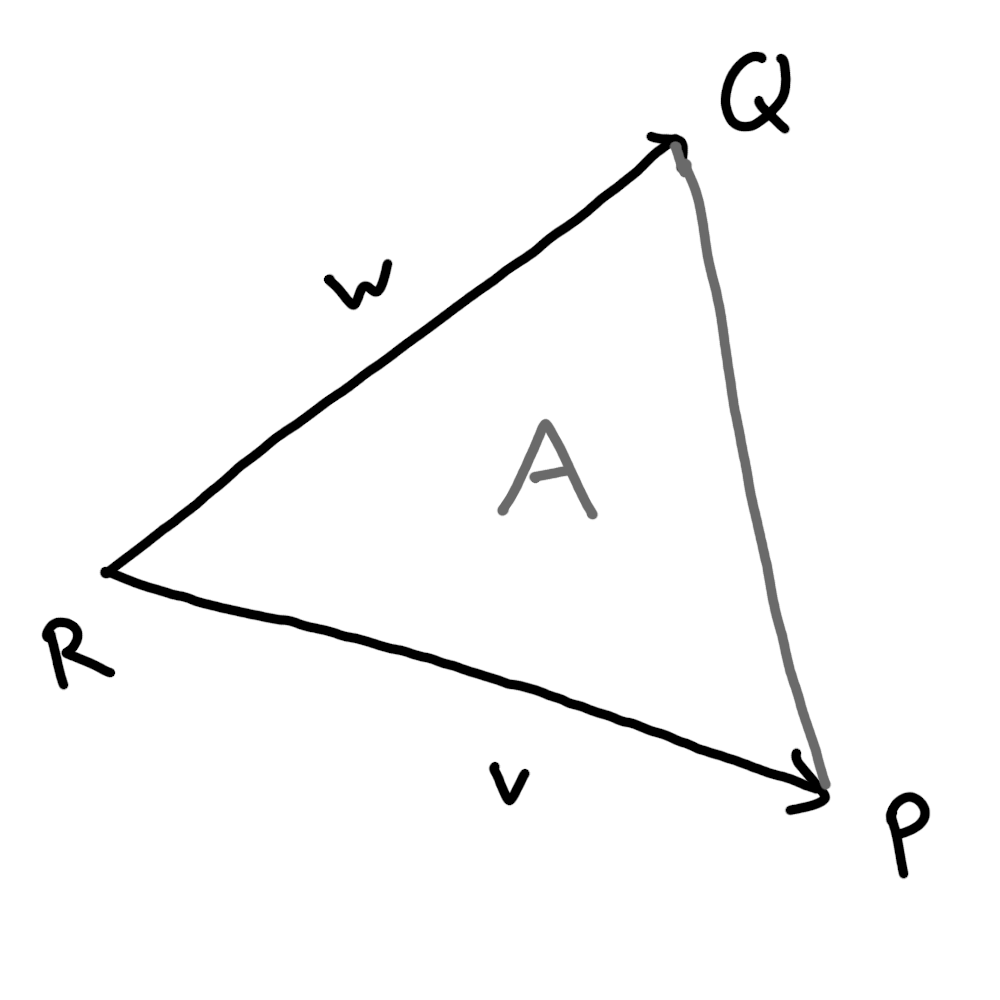
\includegraphics[width=0.3\linewidth]{figures/area_triangle}
		\caption{we want to calculate the area of the triangle between two vectors}
		\label{fig:area_triangle}
	\end{figure}
	
	\begin{align*}
		A = \frac{|\det(v,w)|}{2} = \frac{|\det (P-R, Q-R)|}{2} = \frac{\left|\det\left(\begin{matrix} 1 & R\\ 0 & P-R\\ 0 & Q-R \end{matrix}\right)\right|}{2} = \frac{\left|\det\left(\begin{matrix} 1 & R\\ 1 & P\\ 1 & Q \end{matrix}\right)\right|}{2}
	\end{align*}
\end{remark}

\section{Free form surfaces}

\begin{definition}
	given a control mesh $b_{00}, b_{01}, ..., b_{mn} \in \mathbb{R}^d$, $m,n \in \mathbb{N}$ and two curve schemes $g(s) = \sum_{i=0}^{m}D_i(s)p_i$ and $h(t)=\sum_{j=0}^{n}E_j(t)q_j$.
	
	$f(s,t) := \sum_{i=0}^{m} \sum_{j=0}^{n} D_i(s) E_j(t) b_{ij}$ is called free form surface (also called tensor product surface) (Freiformfläche, Tensorproduktfläche).
\end{definition}

\begin{figure}[h!]
	\centering
	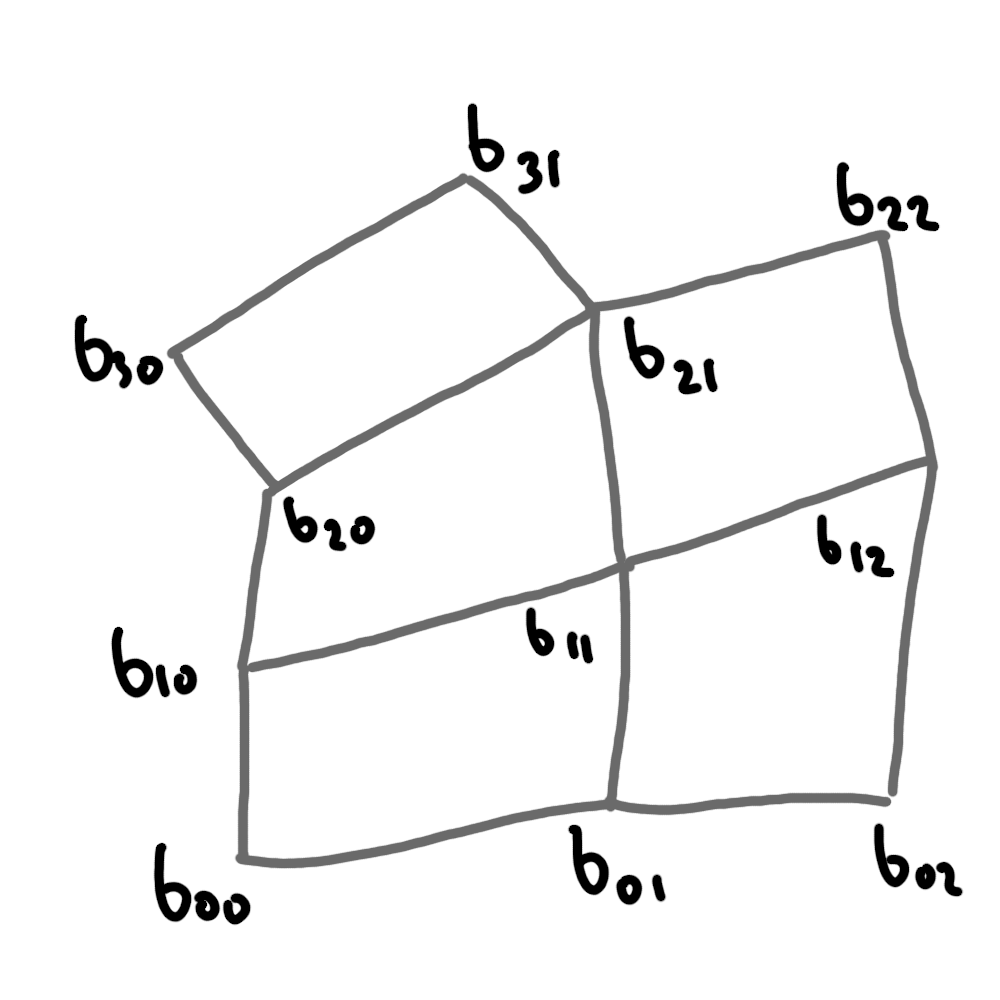
\includegraphics[width=0.3\linewidth]{figures/control_mesh}
	\caption{control mesh}
	\label{fig:control_mesh}
\end{figure}

\begin{example}
	$D_i(s) = B_i^m(s)$ and $E_j(t)=B_j^n(t)$ ... bernstein polynomials then $f(s,t)$ is a bezier surface from degree $(m,n)$.
\end{example}

\begin{example}
	$D_i(s) = N_i^m(s)$ and $E_j(t)=N_j^n(t)$ ... b-spline base functions then $f(s,t)$ is a b-spline surface from degree $(m,n)$.
\end{example}

\begin{lemma}
	\begin{align*}
		f(s,t) = \sum_i \sum_j D_i(s) E_j(t) b_{ij} = \sum_i D_i(s) \underbrace{\sum_i E_j(t) b_{ij}}_{=: h_i(t)} = \sum_i D_i(s)h_i(t)\\
		f(s,t) = ... = \sum_j E_j(t) \underbrace{\sum_i D_i(s) b_{ij}}_{=: g_j(s)} = \sum_j E_j(t) g_j(s)
	\end{align*}
	
	For some $t_0$ $f(s,t_0)$ is called a $s$-parameter line.
	
	$f(s,t_0) = \sum_i D_i(s)\underbrace{h_i(t_0)}_{p_i}$. A $s$-parameter line is a curve of the type $g(s)$. The same is true for $t$-parameter line of type $h(t)$.
\end{lemma}

\begin{example}
	bezier mesh of grade $(2,3)$
	
	\begin{figure}[h!]
		\centering
		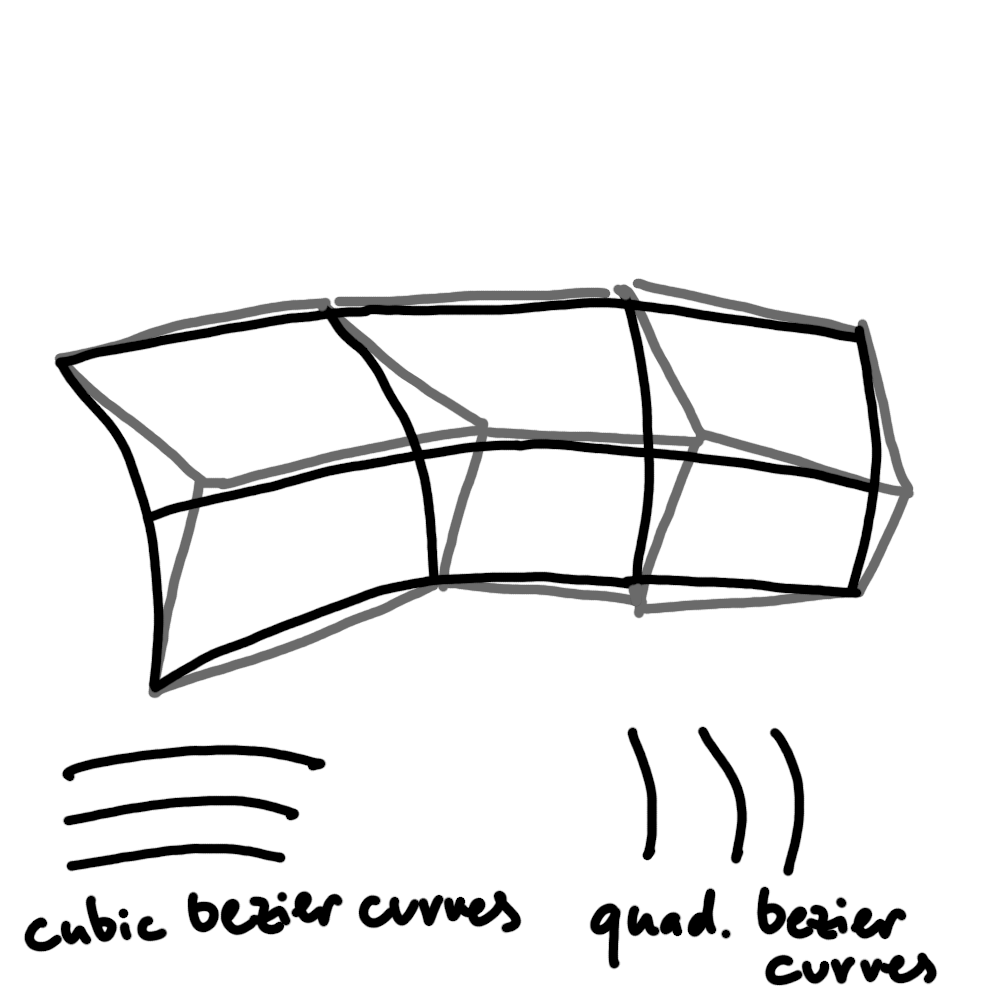
\includegraphics[width=0.3\linewidth]{figures/bezier_mesh}
		\caption{bezier mesh}
		\label{fig:bezier_mesh}
	\end{figure}
\end{example}

\begin{algorithm}[de casteljou for meshes]
	\begin{figure}[h!]
		\centering
		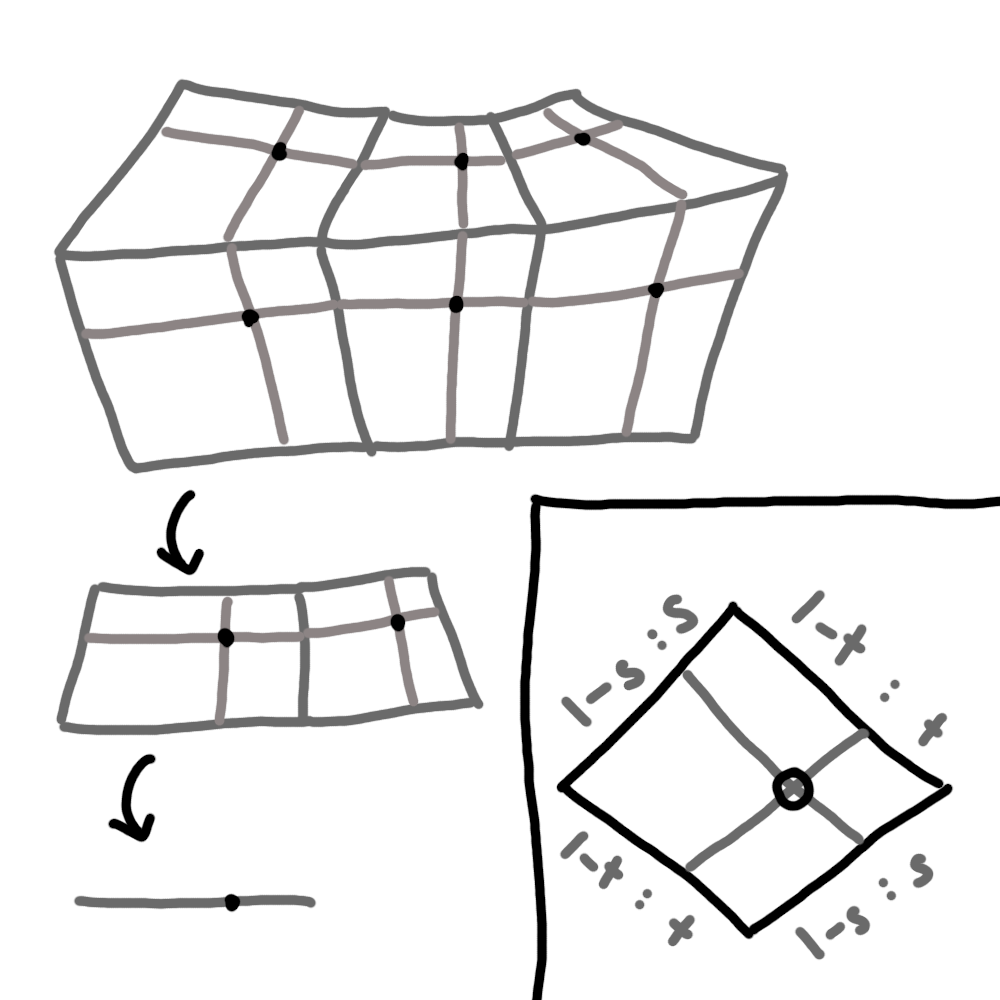
\includegraphics[width=0.3\linewidth]{figures/decasteljou_mesh}
		\caption{cateljou algorithm for meshes}
		\label{fig:decasteljou_mesh}
	\end{figure}
\end{algorithm}

All lemmas and theorems are very similar to free form curves. Therefore we only show selected theorems.

\begin{theorem}
	If $D_i$, $E_i$ are affine invariant, then $f$ is affine invariant.
\end{theorem}

\begin{proof}
	Let $\alpha$ be affine invariant. We have to show $\alpha(f(s,t)) = \sum_i \sum_j D_i(s) E_j(t) \alpha(b_{i,j})$.
	
	\begin{align*}
		\alpha(f(s,t)) = \alpha(\sum_{i=0}^{m} \sum_{j=0}^{n} D_i(s) E_j(t) b_{ij}) = \alpha(\sum_{i=0}^{m}  D_i(s) \overbrace{\sum_{j=0}^{n} E_j(t) b_{ij}}^{h_{ij}}) = \alpha(\sum_{i=0}^{m}  D_i(s) \alpha(h_{ij})) =\\
		\alpha(\sum_{i=0}^{m}  D_i(s) \alpha(\sum_{j=0}^{n} E_j(t) b_{ij})) = \sum_{i=0}^{m} \sum_{j=0}^{n} D_i(s) E_j(t) \alpha(b_{i,j})
	\end{align*}
\end{proof}

Other theorems such as convex hull, end-point-interpolating are analogous.

\section{Subdivision algorithms}

\subsection{Subdivision for curves}

\begin{algorithm}[Chaikin]
	given some polygon $p_i, p_{i+1}, ... \in \mathbb{R}^d$
	
	\begin{enumerate}
		\item copy every vertex $p_i \rightarrow p_i^1$
		\item calculate average of two neighboring $p_i^1$s $m_i^1 = \frac{1}{2}(p_i^1 + p_{i+1}^1)$
		\item average the $m_i^1$s $p_i^2 = \frac{1}{2}(m_i^1 + m_{i+1}^1)$
	\end{enumerate}
	
	The resulting polygon looks similar to the original one, but the corners are rounded. Continue by repeating the procedure with the new polygon as input.
	
	\begin{figure}[h!]
		\centering
		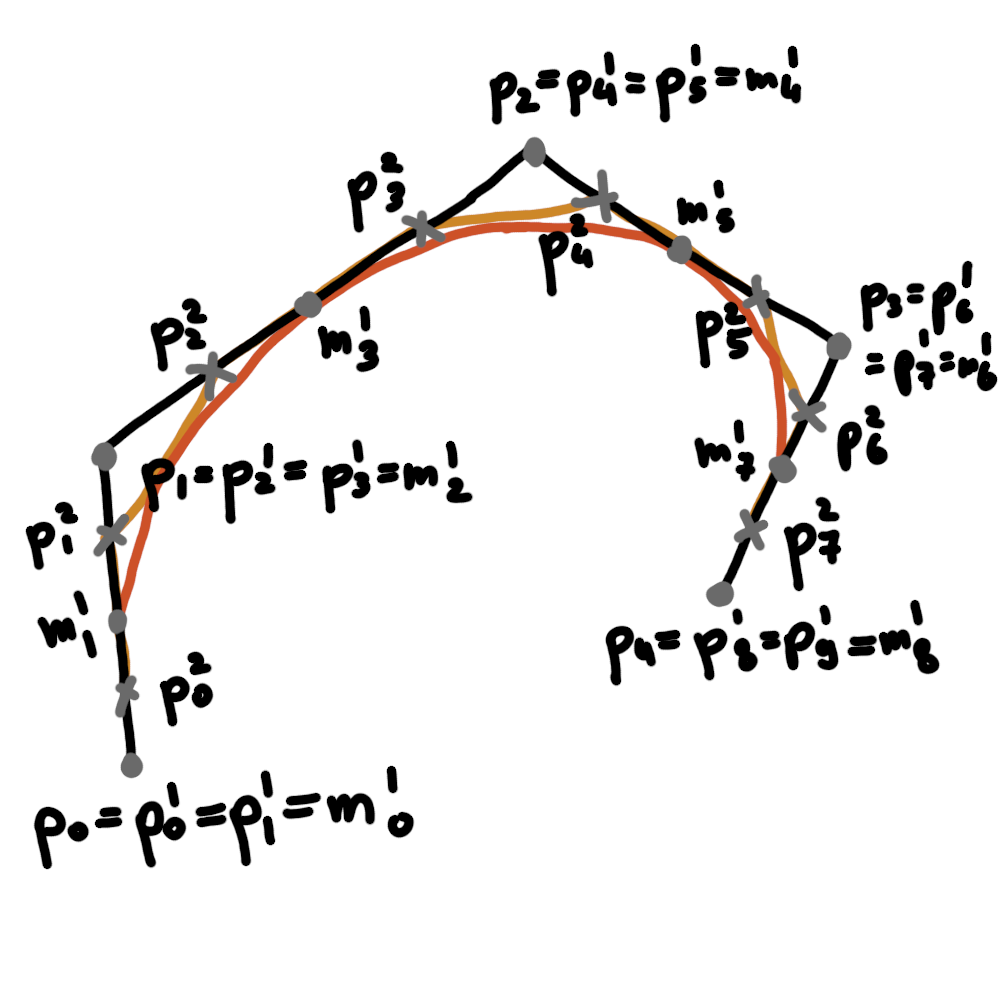
\includegraphics[width=0.3\linewidth]{figures/chaikin}
		\caption{Chaikin algorithm for five given points.}
		\label{fig:chaikin}
	\end{figure}
	
\end{algorithm}

\begin{theorem}
	The algorithm of Chaikin gives polygons that converge to a quadratic B-Spline curve.
\end{theorem}

\begin{remark}
	Remember Chaikin as: copy once, average twice
\end{remark}

\begin{algorithm}[Lane-Riesenfeld]
	same as Chaikin, but copy once, average $n$ times
	
	\begin{figure}[h!]
		\centering
		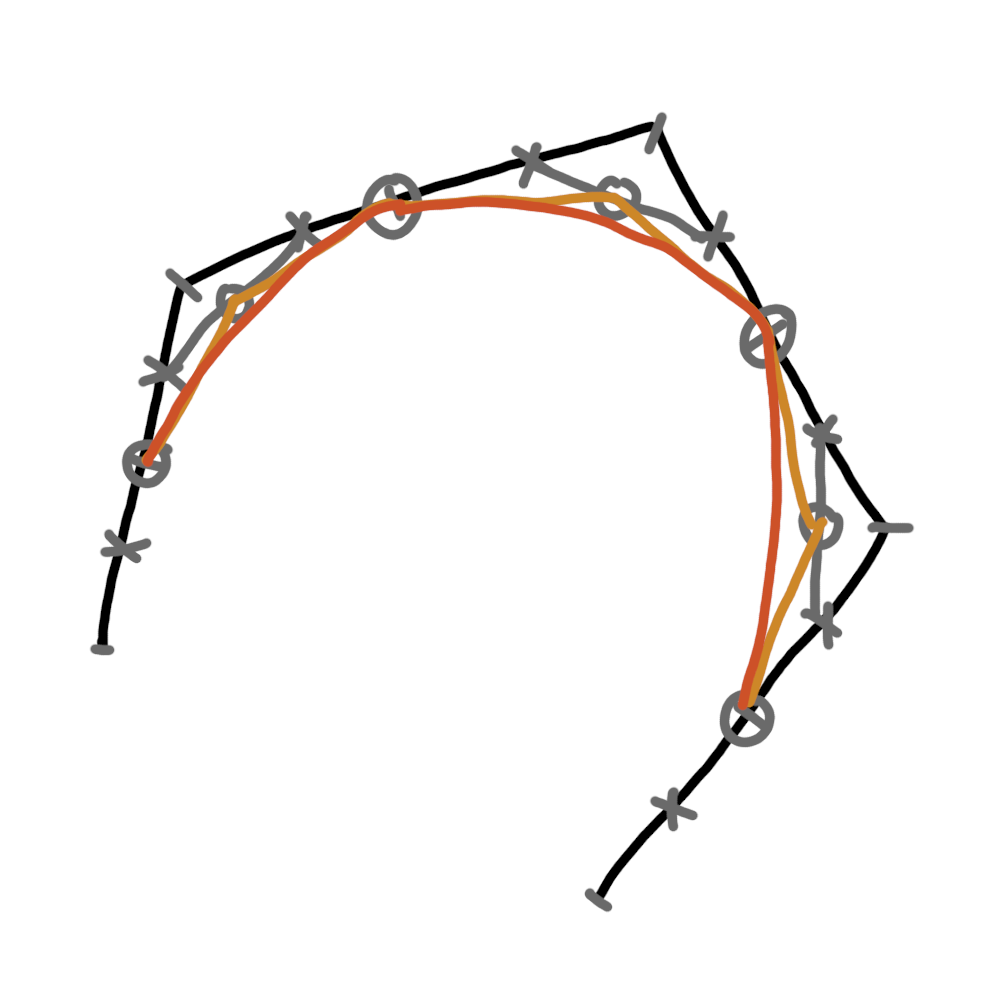
\includegraphics[width=0.3\linewidth]{figures/lane_riesenfeld}
		\caption{Lane Riesenfeld algorithm with $n=3$ for five given points.}
		\label{fig:lane_riesenfeld}
	\end{figure}
\end{algorithm}

\begin{theorem}
	The algorithm of Lane-Riesenfeld gives polygons that converge to a B-Spline curve of degree $n$.
	
	Lane-Riesenfeld is:
	\begin{itemize}
		\item a approximating scheme
		\item is affine invariant.
	\end{itemize}
\end{theorem}

\begin{remark}
	Chaikin is the $n=2$ special case of Lane-Riesenfeld.
\end{remark}

\begin{algorithm}[Four-Point-Scheme]
	\begin{align*}
		p_i^1 := -\frac{1}{16} p_{i-1} + \frac{9}{16} p_i + \frac{9}{16} p_{i+1} - \frac{1}{16} p_{i+2}
	\end{align*}
	
	this is an affine combination. Inductive $p_i^2, ...$.
	
	\begin{figure}[h!]
		\centering
		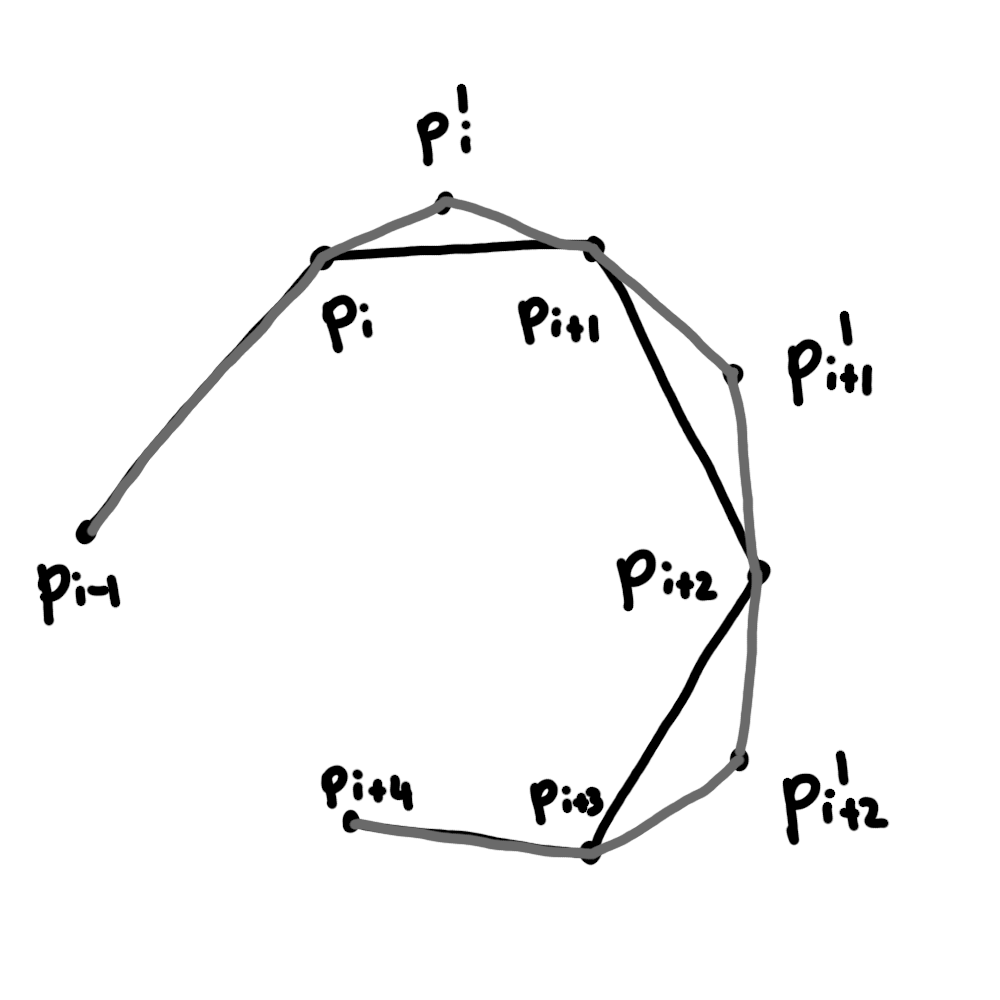
\includegraphics[width=0.3\linewidth]{figures/four_point_scheme}
		\caption{Four Point Scheme for six given points.}
		\label{fig:four_point_scheme}
	\end{figure}
\end{algorithm}

\begin{theorem}
	The curve resulting from the four point scheme converge to a $C^1$ curve.
	
	Four Point Scheme is:
	\begin{itemize}
		\item a interpolating
		\item is affine invariant.
	\end{itemize}
\end{theorem}

\begin{remark}
	The weights of the four point scheme can be chosen differently as well:
	\begin{align*}
		p_i^1 := -w p_{i-1} + (\frac{1}{2} + w) p_i + (\frac{1}{2} w) p_{i+1} - w p_{i+2}
	\end{align*}
	
	Above we choose $w=\frac{1}{16}$. This is always interpolating, but only for $w \in (0, \frac{\sqrt{5} - 1}{8})$ the resulting curve will be $C^1$.
\end{remark}

\begin{remark}
	All of the above schemes preserve sub spaces and therefore have the property of linear precision (lineare Präzesion).
	
	They do not have ''circular precision'', meaning that if all points lie on a sphere then the curve can leave the sphere.
	
	\begin{figure}[h!]
		\centering
		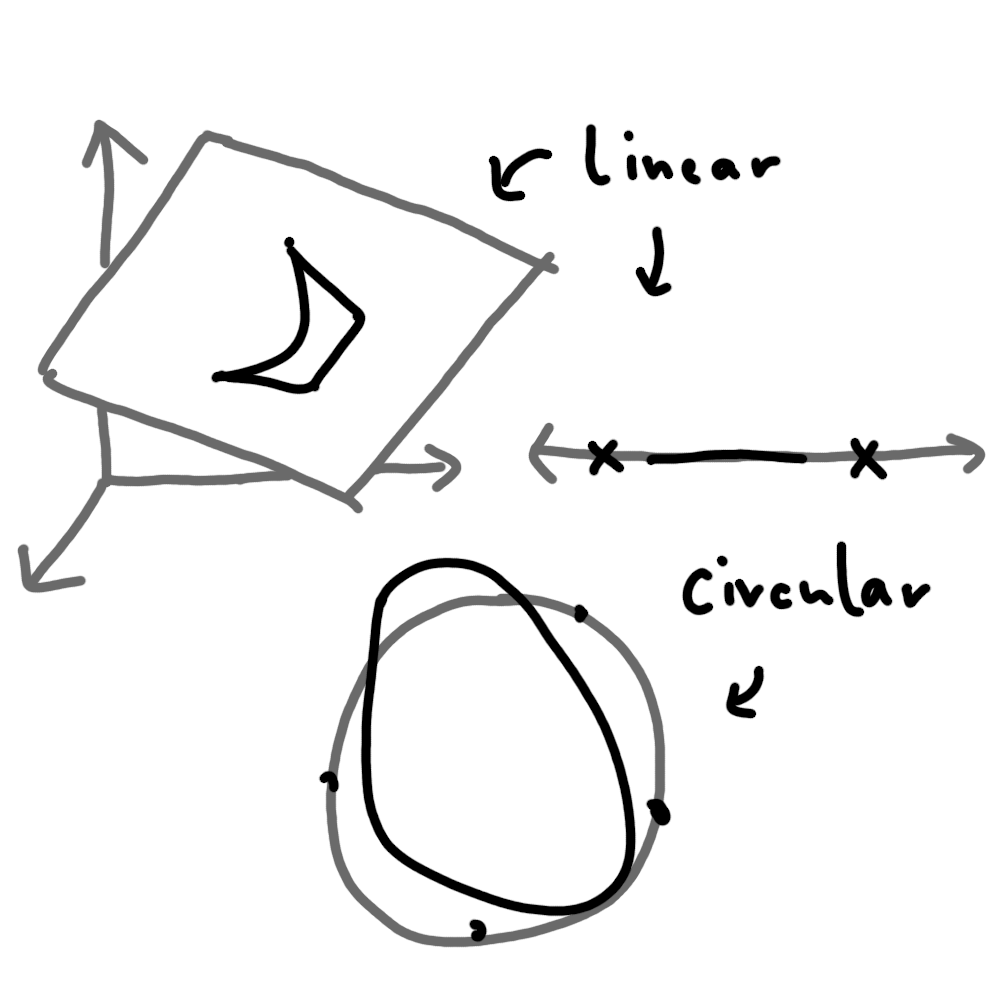
\includegraphics[width=0.3\linewidth]{figures/precision}
		\caption{Example for linear precision, but not circular precision.}
		\label{fig:precision}
	\end{figure}
\end{remark}

\subsection{Subdivision for meshes}

\begin{definition}
	The degree (Valenz) of a vertex is the number of edges connected to the vertex.
\end{definition}

\begin{algorithm}[Loop (triangle meshes)]
	\begin{figure}[h!]
		\centering
		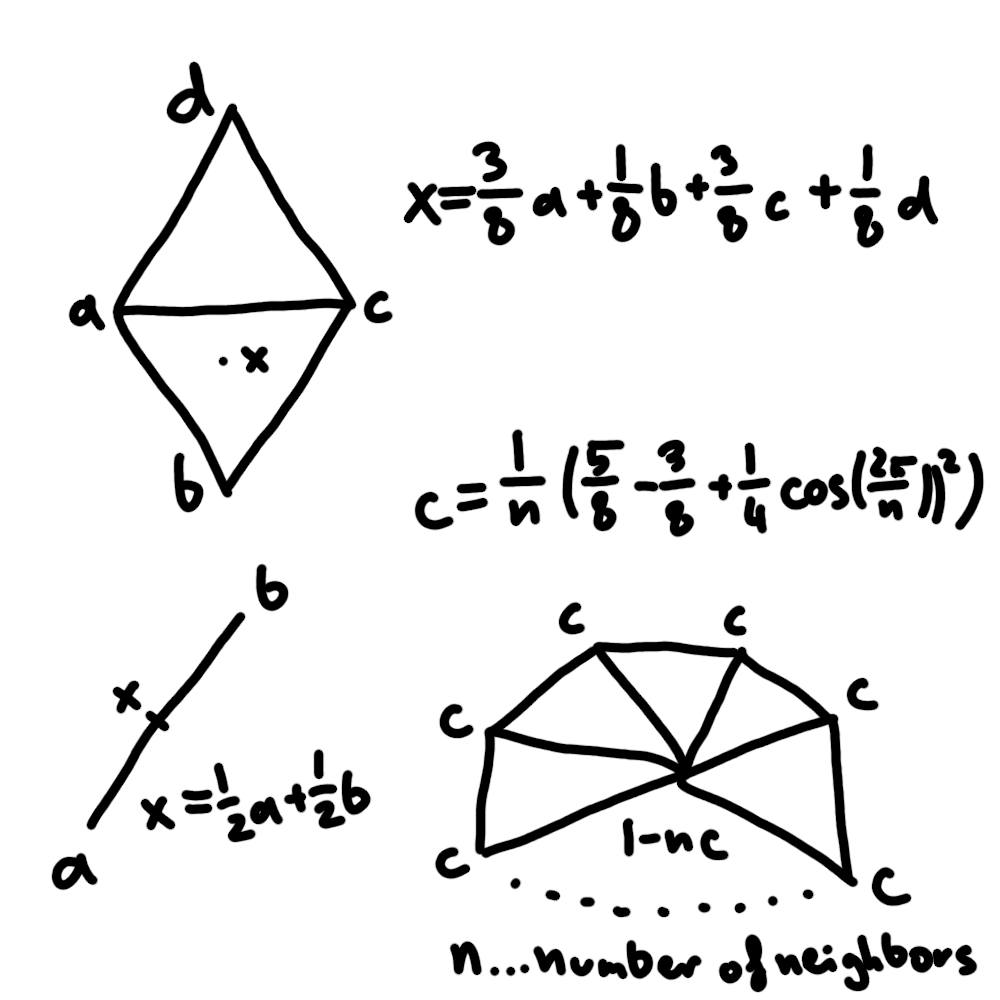
\includegraphics[width=0.3\linewidth]{figures/loop}
		\caption{Loop subdivision.}
		\label{fig:loop}
	\end{figure}
\end{algorithm}

\begin{theorem}
	Loop subdivision
	\begin{itemize}
		\item is approximating
		\item converges to a $C^2$ surface for generic $n=6$ vertices and to a $C^1$ surface otherwise
		\item is face splitting (faces are subdivided)
	\end{itemize}
\end{theorem}

\begin{algorithm}[Modified-Butterfly-Scheme (triangle meshes)]
	\begin{figure}[h!]
		\centering
		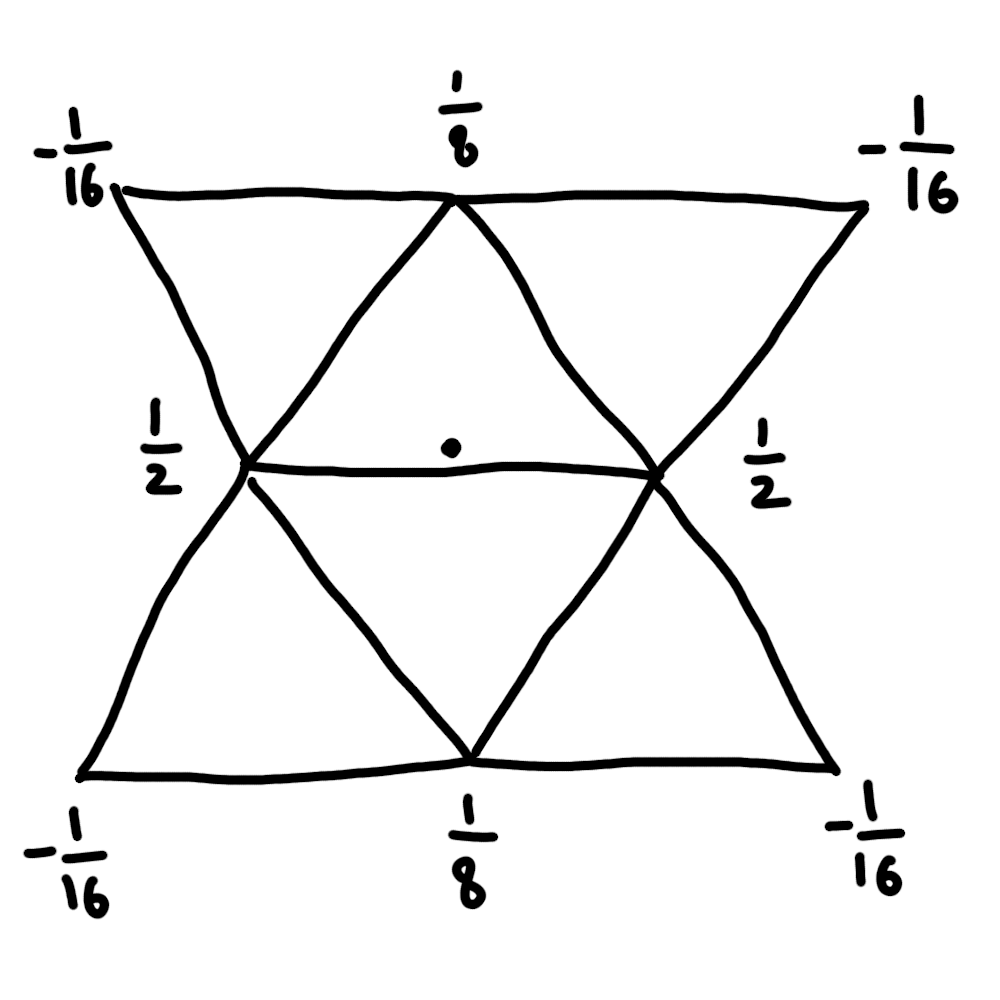
\includegraphics[width=0.3\linewidth]{figures/butterfly}
		\caption{Modified Butterfly subdivision.}
		\label{fig:butterfly}
	\end{figure}
	
	\begin{figure}[h!]
		\centering
		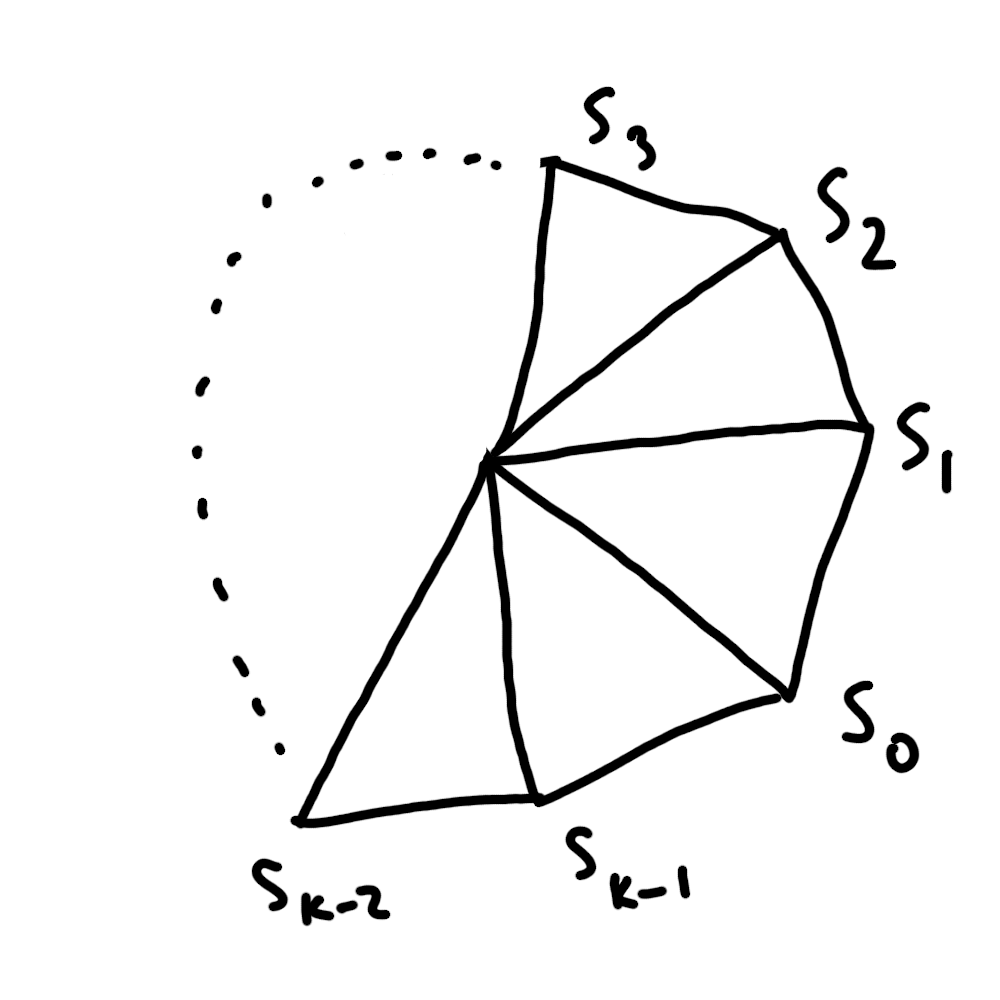
\includegraphics[width=0.3\linewidth]{figures/butterfly_special}
		\caption{Special case in Modified Butterfly subdivision.}
		\label{fig:butterfly_special}
	\end{figure}
	
	As in the image we generate new vertices from edges. For non-generic $k \not= 6$ we specify
	\begin{align*}
		s_j = \frac{1}{k} \left(\frac{1}{4} + \cos\left(\frac{2j\pi}{k}\right) + \frac{1}{2}\cos\left(\frac{4j\pi}{k}\right) \right)
	\end{align*}
	
	\begin{figure}[h!]
		\centering
		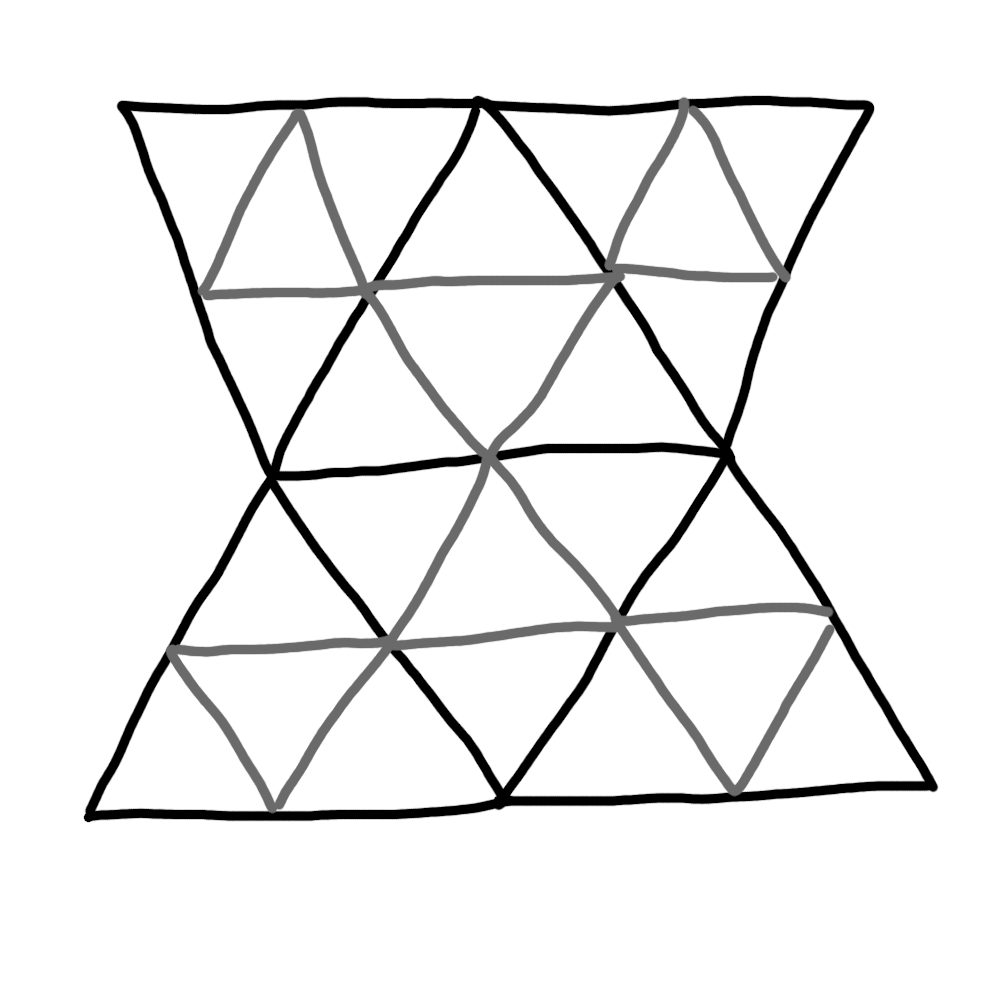
\includegraphics[width=0.3\linewidth]{figures/butterfly_overview}
		\caption{Result of Modified Butterfly subdivision.}
		\label{fig:butterfly_overview}
	\end{figure}
\end{algorithm}

\begin{theorem}
	The Modified Butterfly Scheme:
	\begin{itemize}
		\item is interpolating
		\item converges to a $C^1$ surface
		\item is face-splitting
	\end{itemize}
\end{theorem}

\begin{algorithm}[Catmull-Clark (square meshes)]
	\begin{figure}[h!]
		\centering
		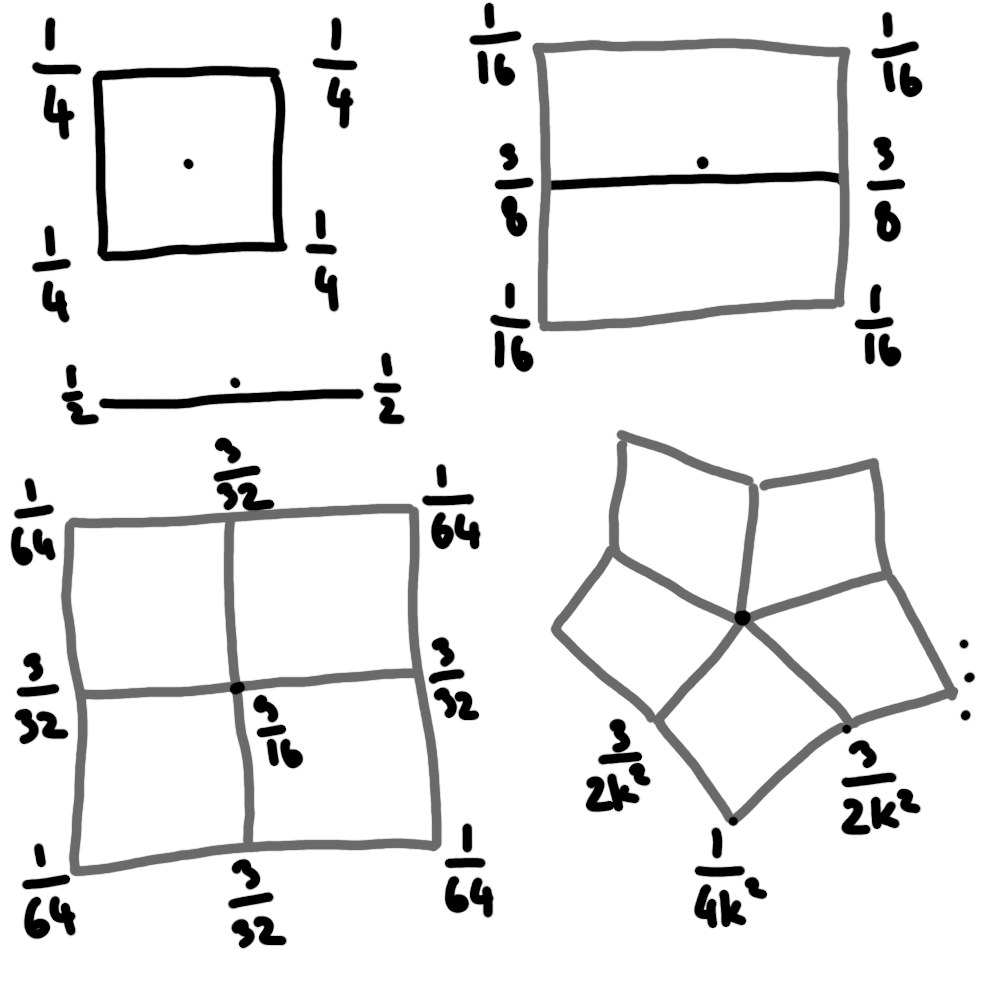
\includegraphics[width=0.3\linewidth]{figures/catmul_clark}
		\caption{Catmul Clark subdivision.}
		\label{fig:catmul_clark}
	\end{figure}
\end{algorithm}

\begin{theorem}
	Catmull Clark is:
	\begin{itemize}
		\item approximating
		\item converges to a $C^2$ surface for generic vertices
		\item is face-splitting
	\end{itemize}
\end{theorem}

\begin{algorithm}[Doo-Sabin]
	\begin{figure}[h!]
		\centering
		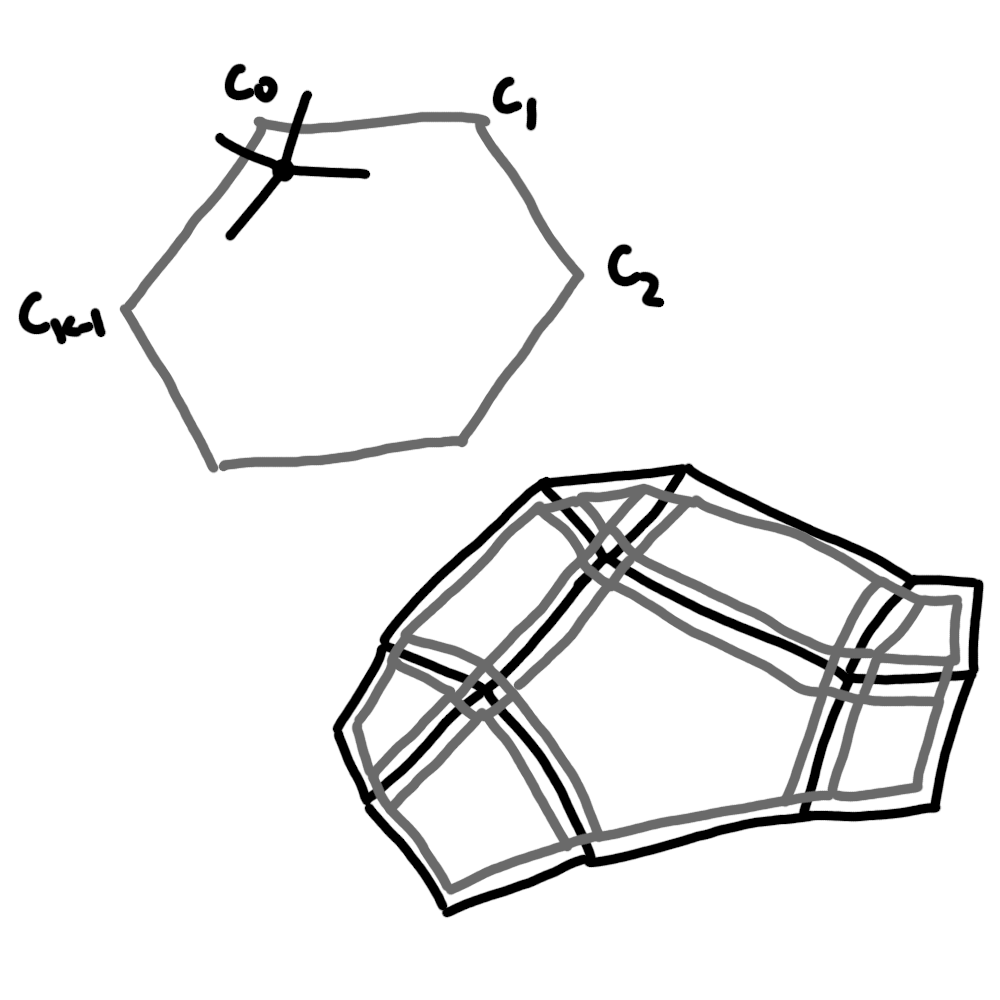
\includegraphics[width=0.3\linewidth]{figures/doo_sabin}
		\caption{Doo Sabin subdivision.}
		\label{fig:doo_sabin}
	\end{figure}
	
	\begin{align*}
		c_j = \frac{\left(3+2\cos\left(\frac{2\pi j}{k}\right)\right)}{4k}, j > 0 && c_0 = \frac{1}{4} + \frac{5}{4k}
	\end{align*}
\end{algorithm}

\begin{theorem}
	Doo-Sabin is:
	\begin{itemize}
		\item approximating
		\item converges to $C^1$ surface
		\item is vertex-splitting.
	\end{itemize}
\end{theorem}

\begin{algorithm}[Kobbelt-Scheme (square meshes)]
	\begin{figure}[h!]
	\centering
	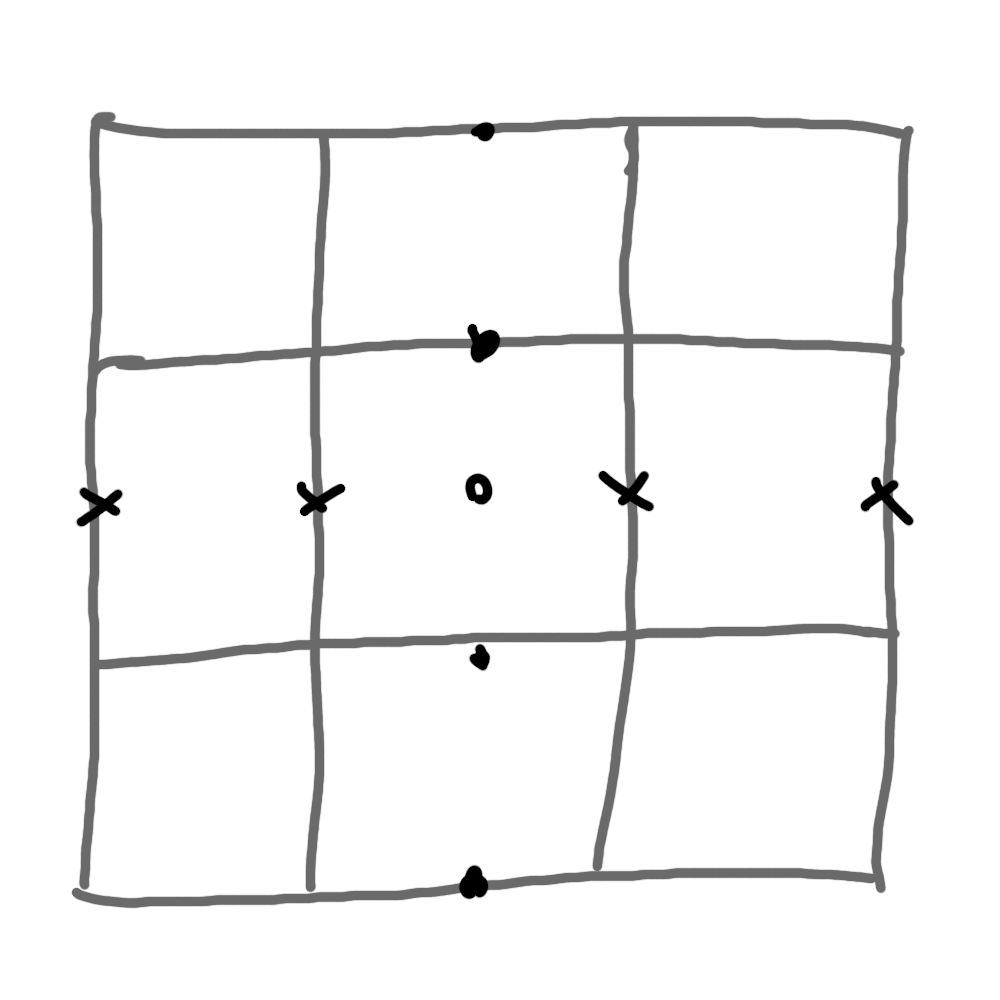
\includegraphics[width=0.3\linewidth]{figures/kobbelt}
	\caption{Kobbelt subdivision.}
	\label{fig:kobbelt}
	\end{figure}

	Apply four-point-scheme for vertical and horizontal vertexes. Then apply four point scheme on resulting points. The ''horizontal'' result and the ''vertical'' result are the same.
\end{algorithm}

\begin{theorem}
	The Kobbelt scheme is:
	\begin{itemize}
		\item interpolating
		\item converges to a $C^1$ surface
		\item is face-splitting.
	\end{itemize}
\end{theorem}

\begin{algorithm}[Half-Edge-Data-Structure]
	given: mesh, that represents a orientable surface.
	
	\begin{figure}[h!]
		\centering
		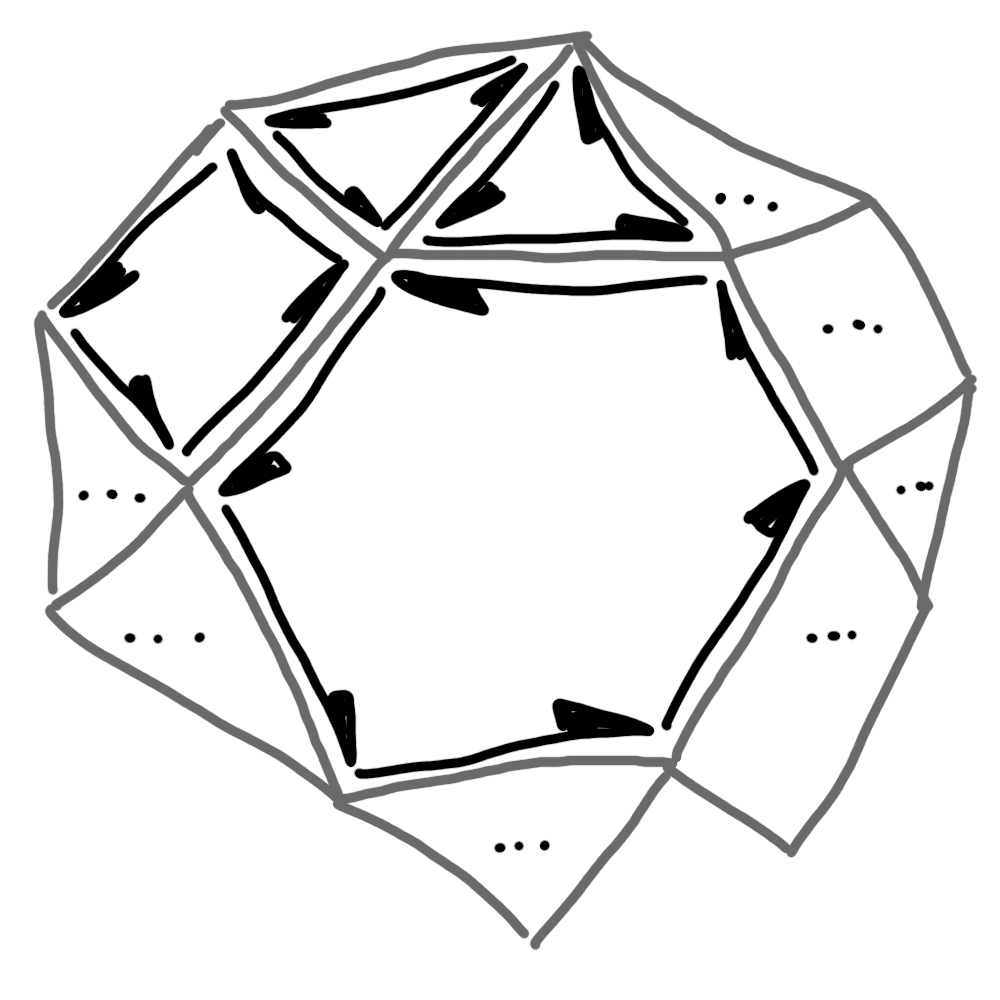
\includegraphics[width=0.3\linewidth]{figures/halfedge}
		\caption{Halfedge datastructure.}
		\label{fig:halfedge}
	\end{figure}
	
	A mesh is a collection of lists. These lists include vertices $v_i$, edges $e_i$, faces $f_i$ and half-edges $h_i$.
	
	Every vertex $v$ is assigned a half-edge \texttt{v->h}. Every face, every edge is assigned a half-edge. Every half-edge is assigned the opposing (\texttt{flip}), next (\texttt{next}), previous (\texttt{prev}) half-edge, the corresponding face (\texttt{f}), vertex (\texttt{v}) and edge (\texttt{e}).
\end{algorithm}

\begin{remark}
	In python use the package \texttt{geopy}. Find it via tiss/Lehrunterlagen. The documentation is at \url{www.geometrie.tuwien.ac.at/kilian/docs/geopy}.
\end{remark}

\section{Conform Pattern Matching}
(Musterübertragung)

\subsection{Euclidean Geometry}

Transformations: Translation, Rotation, Reflection

\begin{figure}[h!]
	\centering
	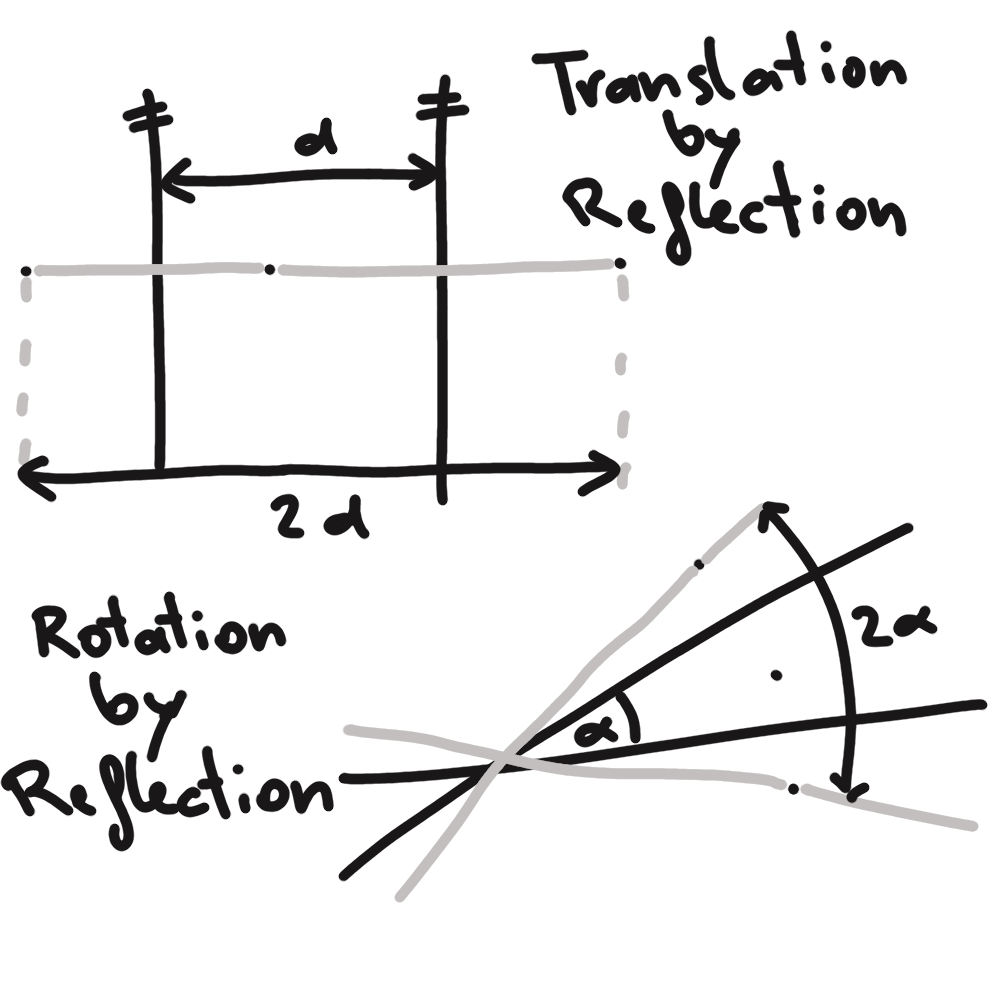
\includegraphics[width=0.3\linewidth]{figures/euclidean_transformation_reflection}
	\caption{Representation of euclidean transformations as reflections.}
	\label{fig:euclidean_transformation_reflection}
\end{figure}

From the figure it follows that euclidean transformations can be represented as reflections along hyper-planes.

\subsection{Möbius Geometry}

\begin{remark}
	This section is closely following the paper Conformal equivalence of triangle meshes by Boris Springborn, Peter Schröder and Ulrich Pinkall from the year 2008.
\end{remark}


\begin{definition}
	Möbius transformations are compositions of reflections along hyper-spheres.
\end{definition}

\begin{definition}[reflection along sphere]	
	\begin{align*}
		\tilde{\omega} := \frac{r^2}{||\omega||^2}\omega
	\end{align*}
\end{definition}

\begin{figure}[h!]
	\centering
	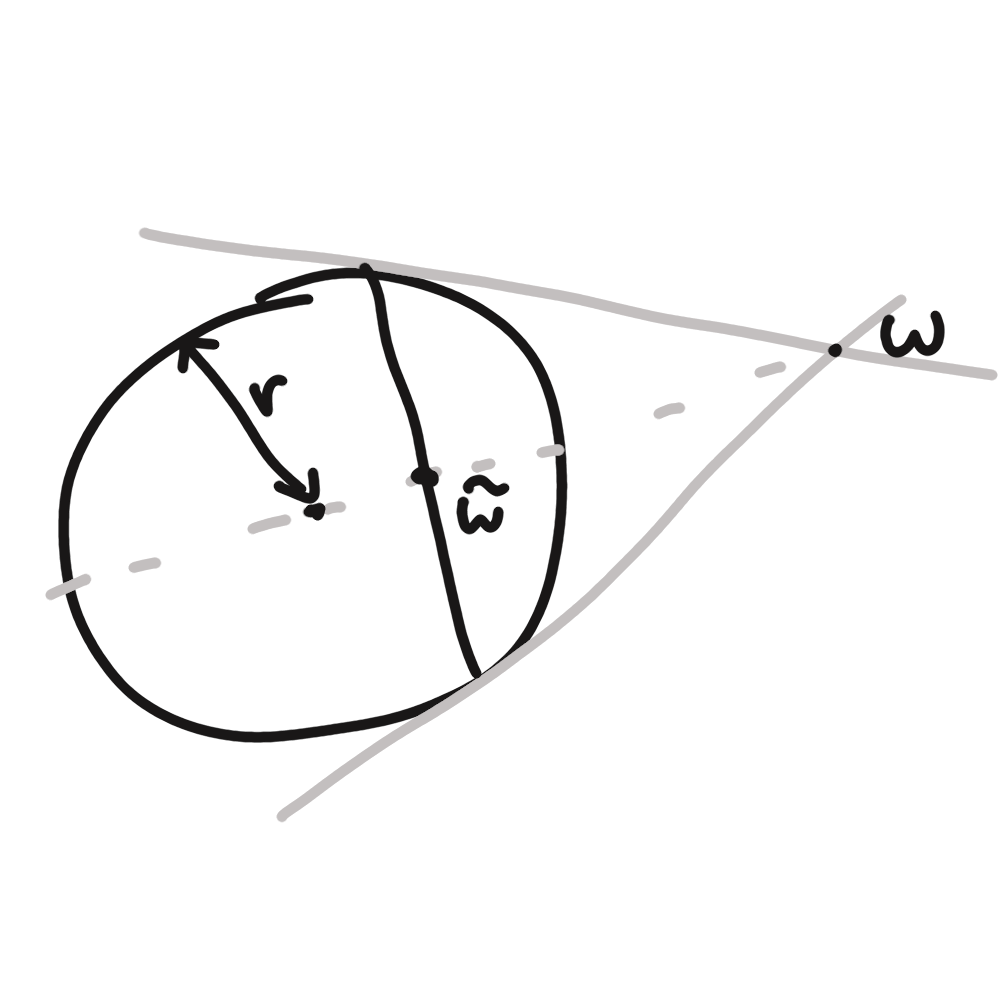
\includegraphics[width=0.3\linewidth]{figures/reflection_on_circle}
	\caption{Reflection of point along a circle.}
	\label{fig:reflection_on_circle}
\end{figure}

\begin{remark}
	Reflecting twice yields the identity.
	
	\begin{align*}
		\tilde{(\tilde{\omega})} = \frac{r^2}{||\tilde{\omega}||^2}\tilde{\omega} = \frac{r^2}{||\frac{r^2}{||\omega||^2}\omega||^2}\frac{r^2}{||\omega||^2}\omega = \frac{r^2}{r^4||\omega||^2}||\omega||^2 r^2 \omega = \omega
	\end{align*}
\end{remark}

Reflecting $\omega$ on a sphere with center $c$ and radius $r$.

\begin{figure}[h!]
	\centering
	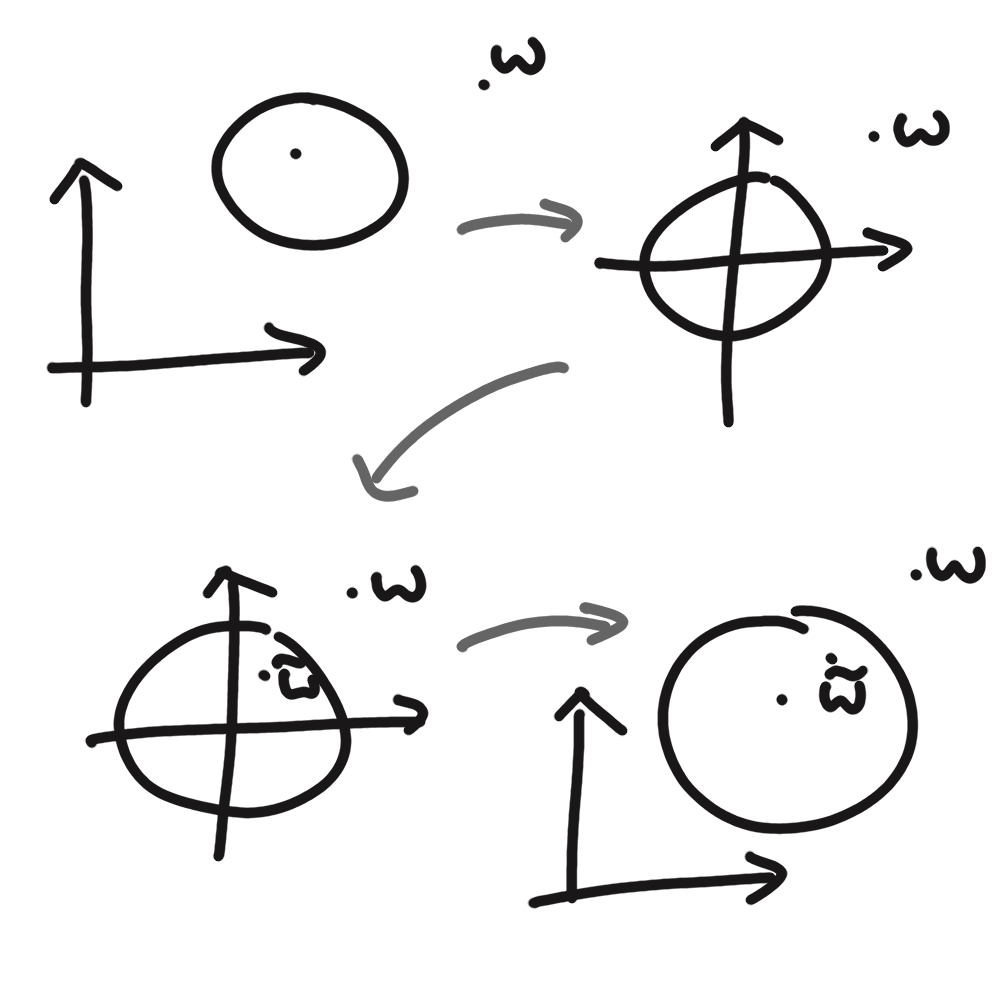
\includegraphics[width=0.3\linewidth]{figures/reflection_on_any_circle}
	\caption{Reflection of point along a circle with different origin.}
	\label{fig:reflection_on_any_circle}
\end{figure}

\begin{align*}
	\tilde{\omega} = \frac{r^2(\omega - c)}{||\omega - c||^2} + c
\end{align*}

\begin{remark}
	Special case: reflection of point $c$: $\tilde{c} := \infty$ and $\tilde{\infty} := c$
\end{remark}

\begin{remark}
	We can identify $\mathbb{R}^2$ with $\mathbb{C}$. Then we get
	
	\begin{align*}
		\tilde{\omega} = \frac{r^2(\omega - c)}{(\omega - c)(\bar{\omega} - \bar{c})} + c = \frac{r^2}{\bar{\omega} - \bar{c}} + c
	\end{align*}
	
	In complex analysis möbius transformations are of the form $m(z) = (az+b)/(cz+d)$ with $a,b,c,d \in \mathbb{C}, ad-bc \neq 0$.  Anti-möbius transformations are $m(z) = (a\bar{z}+b)/(c\bar{z}+d)$.
	
	\begin{align*}
		m(z) = \frac{az+b}{cz+d} = \left(\begin{matrix}
			a & b\\ c & d
		\end{matrix}\right) \left(\begin{matrix}
		z\\ 1
		\end{matrix}\right) = \left(\begin{matrix}
		az+b\\ cz+d
		\end{matrix}\right)
	\end{align*}
	
	Embedding $\mathbb{C} \rightarrow \mathbb{P}(\mathbb{C}) := \{u \subseteq \mathbb{C}^2 | \dim u = 1\}$ with $z \in \mathbb{C} \mapsto [(z, 1)]$ and $[(z_0, z_1)] \mapsto \frac{z_0}{z_1}$, $z_1 \neq 0$.
	
	Then möbius transformations in $\hat{\mathbb{C}} := \mathbb{C} \cup \{\infty\}$ can be represented as a composition of
	
	\begin{itemize}
		\item Rotation: $z \mapsto pz$, with $|p|=1$
		\item Scaling: $z \mapsto Az$, with $A \in \mathbb{R}$
		\item Inversion: $z \mapsto \frac{1}{z}$
		\item Translation: $z \mapsto z + B$, with $B \in \mathbb{C}$
	\end{itemize}

	Proof on Wikipedia.	 
\end{remark}

\begin{definition}[Cross-Ratio (Doppelverhältnis)]
	For $a,b,c,d \in \mathbb{C}$ ... pairwise different we define $DV(a,b,c,d) := \frac{(a-b)(c-d)}{(b-c)(d-a)} \in \mathbb{C}$ as the cross-ratio.
\end{definition}

\begin{example}
	$a,b,c,d \in \mathbb{C}$
	
	\begin{align*}
		DV(a,b,c,d) = \frac{(a-b)}{(c-b)} \frac{(c-d)}{(a-d)} = \frac{r e^{i\phi}}{s e^{i\psi}} \frac{t e^{i\xi}}{u e^{i\nu}} = \frac{r}{s} e^{i(\phi - \psi)} \frac{t}{u} e^{i(\xi - \nu)} = \underbrace{\frac{rt}{su}}_{\in \mathbb{R}} e^{i(\alpha + \beta)}
	\end{align*}
	
	
	\begin{figure}[h!]
		\centering
		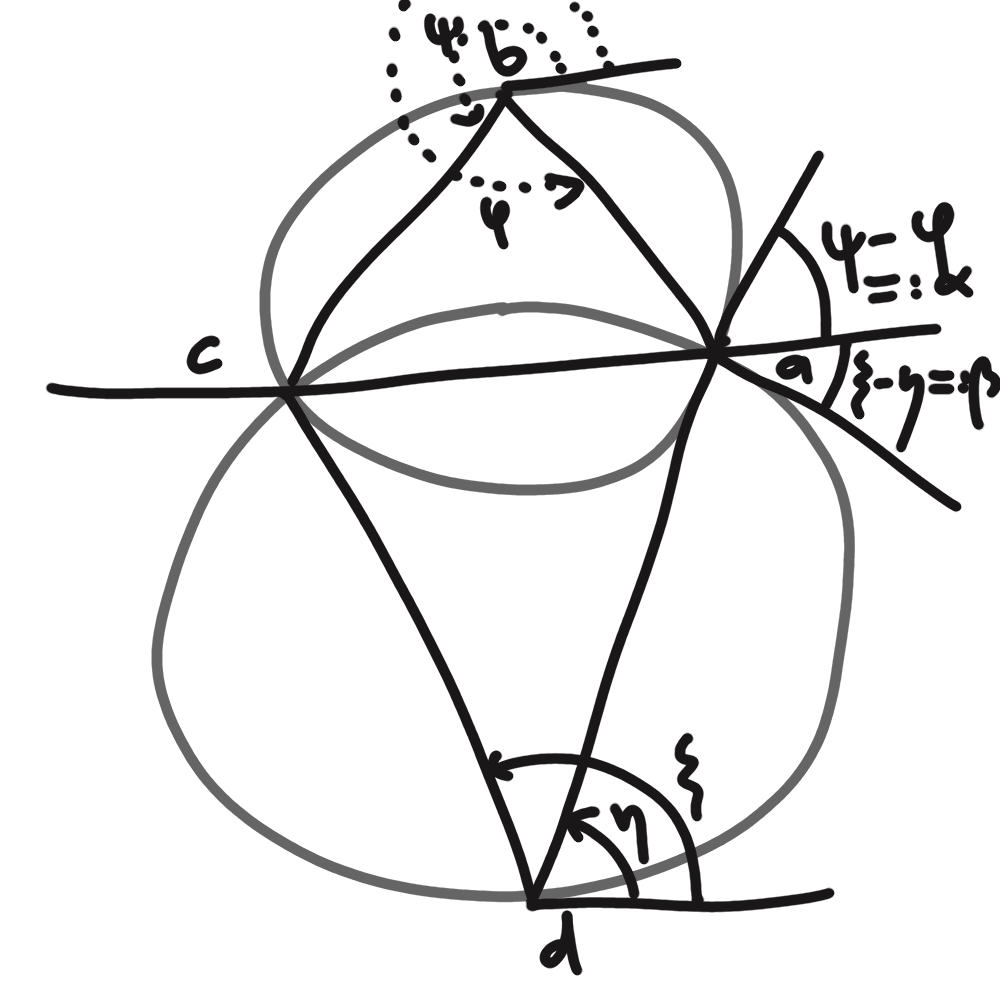
\includegraphics[width=0.3\linewidth]{figures/DV_angle}
		\caption{DV as the angle.}
		\label{fig:DV_angle}
	\end{figure}
	
	The argument of $DV$ is the angle of circumscribed circle of $abc$ and $cda$. As seen in the image.
\end{example}

\begin{remark}
	$DV(a,b,c,d) \in \mathbb{R}$, if and only if they share the circumscribed circle.
	
	\begin{figure}[h!]
		\centering
		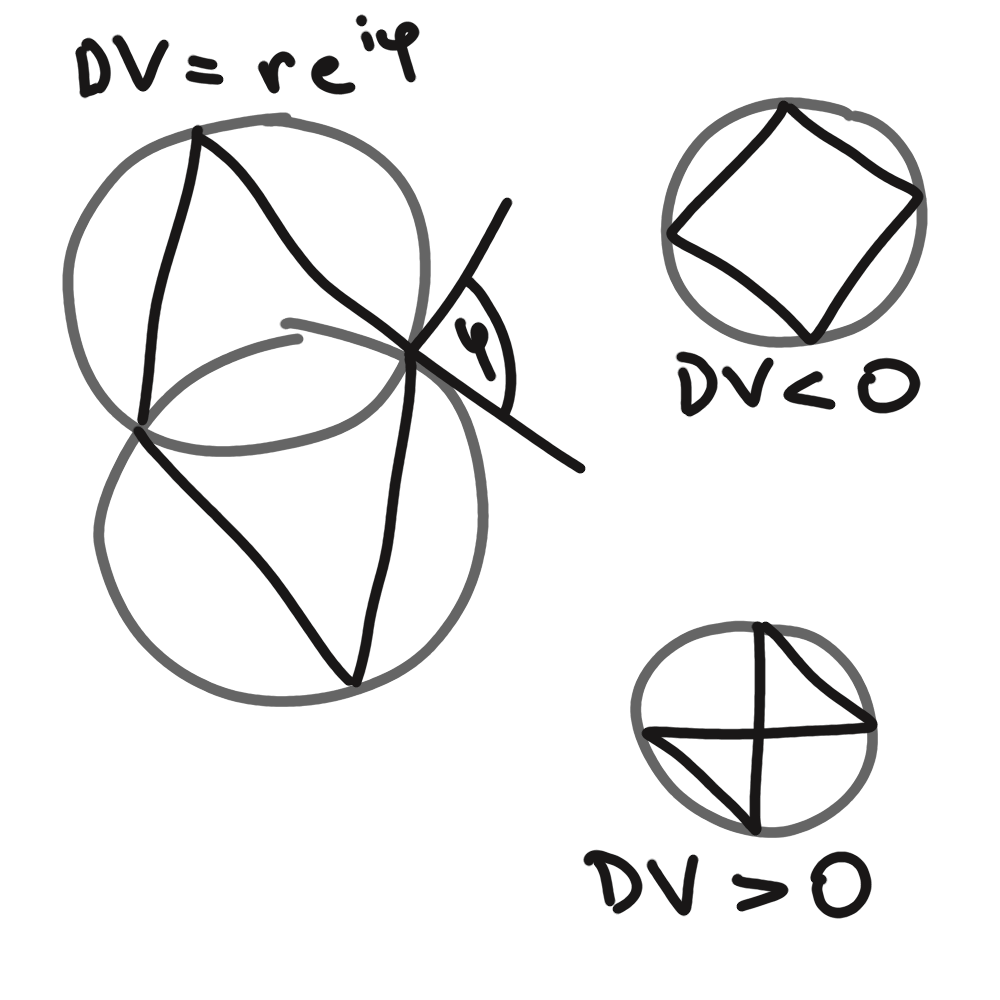
\includegraphics[width=0.3\linewidth]{figures/DV_same_circle}
		\caption{DV and the corresponding angle, as well as examples where the circumscribed circle is shared.}
		\label{fig:DV_same_circle}
	\end{figure}
\end{remark}

\begin{theorem}
	The $DV$ is invariant under all möbius transformations.
\end{theorem}

\begin{proof}
	\begin{itemize}
		\item Scaling:
		\begin{align*}
			DV(Aa, Ab, Ac, Ad)= \frac{(Aa - Ab)(Ac - Ad)}{(Ac - Ab)(Aa - Ad)} = \frac{A(a-b)(c-d)}{A(c-b)(a-d)} = DV(a,b,c,d)
		\end{align*}
		\item Translation:
		\begin{align*}
			DV(a+B, b+B, c+B, d+B)= \frac{((a+B) - (b+B))((c+B) - (d+B))}{((c+B) - (b+B))((a+B) - (d+B))} = DV(a,b,c,d)
		\end{align*}
		\item Rotation: $p=e^{i\phi}, z=r e^{i\psi}$ then $pz=r e^{i(\phi+\psi)}$
		\item Inversion:
		\begin{align*}
			DV\left(\frac{1}{a}, \frac{1}{b}, \frac{1}{c}, \frac{1}{d}\right)= \frac{\left(\frac{1}{a} - \frac{1}{b}\right) \left(\frac{1}{c} - \frac{1}{d}\right) abcd}{\left(\frac{1}{b} - \frac{1}{c}\right) \left(\frac{1}{d} - \frac{1}{a}\right) abcd} = \frac{(b-a)(d-c)}{(c-b)(a-d)} = DV(a,b,c,d)
		\end{align*}
	\end{itemize}
	
	\begin{figure}[h!]
		\centering
		\includegraphics[width=0.3\linewidth]{figures/DV_rotation_invariant}
		\caption{DV is rotation invariant.}
		\label{fig:DV_rotation_invariant}
	\end{figure}
\end{proof}

\begin{theorem}
	Möbius transformations are circle-preserving (kreistreu).
\end{theorem}

\begin{proof}
	$a,b,c,z \in K$ where $K$ is any circle. Then $DV(a,b,c,z) \in \mathbb{R}$. As $DV(m(a), m(b), m(c), m(z)) = DV(a,b,c,z) \in \mathbb{R}$ it follows that $m(a), m(b), m(c), m(z)$ lie on a circle.
\end{proof}

\begin{theorem}
	Möbius transformations are conformal, which means preserving angles (konform, d.h. winkeltreu).
\end{theorem}

\begin{proof}
	
	\begin{figure}[h!]
		\centering
		\includegraphics[width=0.3\linewidth]{figures/moebius_angle_conserving}
		\caption{Corresponding circles are transformed into intersecting circles.}
		\label{fig:moebius_angle_conserving}
	\end{figure}
	
	Consider tangential circles as in the figure. They will be transformed into intersecting circles, as they already are intersecting.
	
	$DV(a,b,c,d) = r e^{i\phi} \implies \phi$ is the angle. $\implies DV(m(a), m(b), m(c), m(d)) = r e^{i\phi}$. Therefore the angle is preserved. 
	
\end{proof}

\begin{remark}
	Holomorphic (holomorphe = komplex diffbare) functions preserve angles, but do not preserve circles.
\end{remark}

\begin{example}
	$z \mapsto sin(z^2)$ is holomorphic, but does not preserve circles.
\end{example}

\begin{remark}
	Möbius transformations are the only conformal, bijective functions from open subsets of $\mathbb{R}^n$, where $n \geq 3$. (Theorem of Liouville).
\end{remark}

\begin{remark}
	Let $a,b,c,d \in Im \mathbb{H}$ (Quaternions) $\cong \mathbb{R}^3$.
	
	$DV(a,b,c,d) = (a-b) (b-c)^{-1} (c-d) (d-a)^{-1}$ as $\mathbb{H}$ is not commutative (Schiefkörper).
	
	It still holds that $DV(a,b,c,d) \in \mathbb{R} \iff a,b,c,d$ lie on a common circle.
\end{remark}

\begin{definition}	
	$f, \tilde{f}$... bijective, $\phi:f(U) \rightarrow \tilde{f}(U), x \mapsto \tilde{f} \circ f^{-1}(x)$.
	
	$\phi$ is described over $f, \tilde{f}$ by the same parameter (durch den gleichen Parameter beschrieben).
\end{definition}



We ask our-self when $\phi$ is isometric (isometrisch = längentreu).

\begin{definition}[preserving length]
	$\phi$ is preserving length $\iff \forall $ curves $c$ in $f(U):$ $\phi(c)$ is as long as $c$
	
	$c:I \rightarrow \mathbb{R}^3$ ... curve, then the length of $c$ is defined by $L(c) := \int_{I} ||\dot{c}(t)|| dt$
\end{definition} 

\begin{figure}[h!]
	\centering
	\includegraphics[width=0.3\linewidth]{figures/preserving_length}
	\caption{Definition preserving length.}
	\label{fig:preserving_length}
\end{figure}	

\begin{lemma}
	$\phi$ is isometric $\iff \forall \gamma : I \rightarrow U: L(f \circ \gamma) = L(\phi(f \circ \gamma))$.
\end{lemma}

\begin{proof}
	\begin{align*}
		||\dot{c}(t)||^2 = ||\frac{dc(t)}{dt}||^2 = || fu \dot{\gamma_1} + fv \dot{\gamma_2}||^2 = <\dot{\gamma_1}fu + \dot{\gamma_2} fv + \dot{\gamma_1}fu + \dot{\gamma_2} fv> =\\
		\dot{\gamma_1}^2 \underbrace{<fu, fu>}_{=E} + 2 \dot{\gamma_1} \dot{\gamma_2} \underbrace{<fu, fv>}_{=F} + \dot{\gamma_2}^2 \underbrace{<fv, fv>}_{=G} = (\dot{\gamma_1}, \dot{\gamma_2}) \left(\begin{matrix}
			E & F\\ F & G
		\end{matrix}\right) \left(\begin{matrix}
		\dot{\gamma_1} \\ \dot{\gamma_2}
		\end{matrix}\right) = \dot{\gamma}^T \underbrace{\left(\begin{matrix}
			E & F\\ F & G
		\end{matrix}\right)}_{=I} \dot{\gamma}
	\end{align*}
	
	$I$ is matrix of first fundamental form (1. Fundamentalform).
	
	$\implies ||\dot{c}(t)||^2 = \dot{\gamma}^T I \dot{\gamma}$. Therefore $L(c) = \int_{a}^{b} \sqrt{\dot{\gamma}^T I \dot{\gamma}}dt$
	
	$\phi$ is preserving length $\iff \forall \gamma: L(f\circ \gamma) = L(\phi(f \circ \gamma))$
	
	$\gamma:(a,b) \rightarrow U, t \mapsto q + (t_0+t, 0)^T$.
	
	\begin{align*}
		L(f \circ \gamma) = \int_{a}^{b} \sqrt{(1, 0) \left(\begin{matrix}
				E & F \\ F & G
			\end{matrix}\right) \left(\begin{matrix}
			1 \\ 0
			\end{matrix}\right)} dt = \int_{a}^{b} \sqrt{E} dt\\
		L(\phi(f \circ \gamma)) = \int_{a}^{b} \sqrt{\tilde{E}} dt\\
		\tilde{E} = <\tilde{f}u, \tilde{f}u>, \tilde{F} = <\tilde{f}u, \tilde{f}v>, \tilde{G} = <\tilde{f}v, \tilde{f}v>
	\end{align*}
	
	$\phi$ is preserving length $\iff \forall a,b: \int_{a}^{b} \sqrt{E} dt = \int_{a}^{b} \sqrt{\tilde{E}} dt \iff \sqrt{E} = \sqrt{\tilde{E}} \iff E = \tilde{E} (\iff <fu, fu> = <\tilde{f}u, \tilde{f}u>)$.
	
	Analogous $\gamma(t) = q + (0, t_0+t)^T \implies G = \tilde{G}$.
	
	\begin{align*}
		\gamma(t) = q + \left(\begin{matrix}
			t_0 + t \\ t_1 + t
		\end{matrix}\right) \implies \sqrt{E + 2F + G} = \sqrt{\tilde{E} + 2\tilde{F} + \tilde{G}}\\
		E+2F+G = ||fu||^2 + 2 <fu, fv> + ||fv||^2 \geq ||fu||^2 - 2||fu||\cdot ||fv|| + ||fv||^2 = (||fu||- ||fv||)^2\\
		\implies F = \tilde{F}
	\end{align*}
	
	$\implies \phi$ is preserving length $\implies I = \tilde{I}$ and $I = \tilde{I} \implies \phi$ is preserving length.
\end{proof}

\begin{theorem}
	$\phi$ is preserving area $\iff \det I = \det \tilde{I}$.
\end{theorem}

\begin{proof}
	without proof.
\end{proof}

\begin{corollary}
	preserving length $\implies I = \tilde{I} \implies \det I = \det \tilde{I} \implies$ preserving area.
\end{corollary}

\begin{theorem}
	$\phi$ is conformal (preserving angles) $\iff \exists \lambda: \mathbb{R} \rightarrow \mathbb{R}\setminus\{0\}: I = \lambda^2 \tilde{I}$.
\end{theorem}

\begin{remark}
	preserving length $\iff$ preserving angles and preserving area.
	
	\begin{figure}[h!]
		\centering
		\includegraphics[width=0.3\linewidth]{figures/no_length_preserving_exists}
		\caption{There exists no such length preserving $\phi$.}
		\label{fig:no_length_preserving_exists}
	\end{figure}	
	
	Stereographic projection are preserving angles.
	
	\begin{figure}[h!]
		\centering
		\includegraphics[width=0.3\linewidth]{figures/stereographic_projection}
		\caption{Stereographic projections are preserving angles.}
		\label{fig:stereographic_projection}
	\end{figure}	
\end{remark}

\begin{definition}[Triangle mesh]
	Triangle mesh = polyhedral area (local like open subset of $\mathbb{R}^2$) and all areas are triangles.
	
	$T=(V,E,F)$ where $V$ ... vertices, $E$ ... edges, $F$ ... faces
\end{definition}

\begin{figure}[h!]
	\centering
	\includegraphics[width=0.3\linewidth]{figures/triangle_mesh}
	\caption{Triangles mesh (top) and ones consisting of triangles that are not triangle meshes (bottom).}
	\label{fig:triangle_mesh}
\end{figure}	

\begin{remark}
	$\forall$ polyhedron (Polyeder) that are homeomorph (homöomorph): $F-E+V=2$.
\end{remark}

\begin{definition}
	A function $L:E \rightarrow \mathbb{R}_{\geq 0}$ for which $\forall f \in F:$ $f$ satisfies the triangle equations, is called discrete metric (diskrete Metrik) auf $T$.
	
	The triangle equations are given by:
	\begin{align*}
		l_{ij} = l(v_i, v_j) \text{... length of the edge between } v_i and v_j\\
		l_{ij} \leq l_{jk} + l_{ki}\\
		l_{jk} \leq l_{ki} + l_{ij}\\
		l_{ki} \leq l_{ij} + l_{jk}\\
		l_{ij} = l_{ji} \forall i, j, k
	\end{align*}
\end{definition}

\begin{figure}[h!]
	\centering
	\includegraphics[width=0.3\linewidth]{figures/discrete_metric}
	\caption{Vertices associated to face $f$ in definition of discrete metric.}
	\label{fig:discrete_metric}
\end{figure}	

\begin{example}
	The ''true'' lengths $l_{ij} = ||v_i - v_j||$ of the edges form a discrete metric.
\end{example}

\begin{definition}
	Two combinatorial equivalent triangle meshes $T, \tilde{T}$ are called discrete conform equivalent (diskret konform äquivalent), if $\exists \lambda: E \rightarrow \mathbb{R}_{\geq 0}$ with $\tilde{l}_{ij} = \lambda_i \lambda_j l_{ij} \forall (i,j) \in E$.
\end{definition}

\begin{lemma}
	Let $m$ be a möbius tranformation $m:\mathbb{R}^n \cup \{\infty\} \rightarrow \mathbb{R}^n \cup \{\infty\}$.
	
	$\implies \exists \rho:\mathbb{R}^n \rightarrow \mathbb{R}_{\geq 0}: ||m(x)-m(y)|| = \rho(x) \rho(y) ||x-y||$.
\end{lemma}

\begin{proof}
	without proof
\end{proof}

\begin{definition}
	length cross-ration (Längendoppelverhältnis) $LDV(v_i, v_j, v_k, v_m) := \frac{l_{ij}l_{km}}{l_{jk}l_{mi}}$
\end{definition}

\begin{figure}[h!]
	\centering
	\includegraphics[width=0.3\linewidth]{figures/length_cross_ratio}
	\caption{Definition of length cross ratio.}
	\label{fig:length_cross_ratio}
\end{figure}

\begin{remark}
	$a,b,c,d \in \mathbb{C}$ then $LDV(a,b,c,d) = |DV(a,b,c,d)|$
\end{remark}

\begin{theorem}
	$(T,l)$ and $(\tilde{T}, \tilde{l})$ are discrete conform equivalent $\iff \forall ik \in E: LDV(v_i, v_j, v_k, v_m) = LDV(\tilde{v_i}, \tilde{v_j}, \tilde{v_k}, \tilde{v_m})$.
\end{theorem}

\begin{theorem}
	Let $T$ be a triangle mesh with metric $l_{ij} := ||v_i - v_j||$. Let $m$ be a möbius transformation. Then $T$ and $\tilde{T}$ are conform equivalent.
\end{theorem}

\begin{remark}
	In the above theorem we means that when the edges are möbius transformed and then connected with straight edges to get a triangle mesh.
	
	\begin{figure}[h!]
		\centering
		\includegraphics[width=0.3\linewidth]{figures/moebius_transformation_triangle_mesh}
		\caption{Möbius transformation of the triangle mesh.}
		\label{fig:moebius_transformation_triangle_mesh}
	\end{figure}
\end{remark}

\begin{proof}
	use the above lemma.
\end{proof}

\begin{remark}
	In a plane möbius transformations are uniquely given by three points.
\end{remark}

\begin{definition}[(Milnov's) Lobachevsky-Function]
	\begin{align*}
		 \Pi(x) := \int_{0}^{x} \log |2\sin(t)| dt
	\end{align*}
	
	Cyrillic L looks like $\Pi$.
\end{definition}

\begin{lemma}
	Properties of $\Pi(x)$:
	\begin{itemize}
		\item $\Pi(0) = 0$
		\item $\Pi(x+\pi) = \Pi(x)$ ... pi-periodic
		\item $\Pi(k\pi) = 0$
		\item $\Pi(-x) = -\Pi(x)$
	\end{itemize}
\end{lemma}

\begin{definition}
	\begin{align*}
		M := \{(x,y,z) \in \mathbb{R}^3 | e^x, e^y, e^z \text{ are the lengths of sides of a trianlge}\} =\\
		\{(x,y,z) \in \mathbb{R}^3| e^x \leq e^y + e^z, e^y \leq e^x + e^z, e^z \leq e^x + e^y\}\\
		\\
		f(x,y,z) := \alpha x + \beta y + \gamma z + \Pi(\alpha) + \Pi(\beta) + \Pi(\gamma)
	\end{align*}
	
	where $\alpha(x,y,z), \beta(x,y,z), \gamma(x,y,z)$ are the angles of the triangle. $x,y,z \in M$.
\end{definition}

\begin{figure}[h!]
	\centering
	\includegraphics[width=0.3\linewidth]{figures/definition_M}
	\caption{Definition of M and corresponding angles.}
	\label{fig:definition_M}
\end{figure}

\begin{lemma}
	\begin{align*}
		\frac{\delta f}{\delta x} = \alpha && \frac{\delta f}{\delta y} = \beta && \frac{\delta f}{\delta z} = \gamma
	\end{align*}
\end{lemma}

\begin{proof}
	\begin{align*}
		\frac{\delta f}{\delta x} = \frac{\delta \alpha}{\delta x} x + \alpha + \frac{\delta \beta}{\delta x} y + \frac{\delta \gamma}{\delta x}z + (- \log |2\sin(\alpha)|) \frac{\delta \alpha}{\delta x} + (-\log |2\sin(\beta)|) \frac{\delta \beta}{\delta x} + (- \log(|2\sin\gamma)|) \frac{\delta \gamma}{\delta x} =\\
		\alpha + \frac{\delta \alpha}{\delta x}(x-\log(|2\sin\alpha|)) + \frac{\delta \beta}{\delta x}(y-\log(|2\sin\beta|)) + \frac{\delta \gamma}{\delta x}(z-\log(|2\sin\gamma|)) = ...
	\end{align*}
	
	We do a short calculation on the side:
	
	\begin{align*}
		\sin(\alpha) = \frac{\frac{e^x}{2}}{R} \implies 2 R \sin(\alpha) = e^x \implies R = \frac{e^x}{|2 \sin(\alpha)|} \implies \log R = x - \log|2\sin(\alpha)|
	\end{align*}
	
	\begin{figure}[h!]
		\centering
		\includegraphics[width=0.3\linewidth]{figures/proof_deviation_f}
		\caption{Figure for side calculation.}
		\label{fig:proof_deviation_f}
	\end{figure}
	
	Which gives us
	
	\begin{align*}
		... = \alpha + \frac{\delta \alpha}{\delta x} \log R + \frac{\delta \beta}{\delta x} \log R + \frac{\delta \gamma}{\delta x} \log R = \alpha + \log R (\frac{\delta (\alpha + \beta + \gamma)}{\delta x}) = \alpha + \log R \underbrace{(\frac{\delta \Pi}{\delta x})}_{=0} = \alpha
	\end{align*}
\end{proof}

\begin{remark}
	Discrete conform equivalent $\tilde{l}_{ij} = \lambda_i\lambda_j l_{ij}$ in different wording:
	
	$\exists \lambda_i > 0 \implies \exists u_i : \lambda_i = e^{\frac{u_i}{2}}$ with $u_i \in \mathbb{R}$.
	
	$\gamma_{ij} := \log l_{ij}$, $\tilde{\gamma}_{ij} := \log \tilde{l}_{ij}$ gives us
	
	$\log \tilde{l}_{ij} = \log \lambda_i + \log \lambda_j + \log l_{ij} \iff \tilde{\lambda}_{ij} = \frac{u_i}{2} + \frac{u_j}{2} + \gamma_{ij}$
	
	which is an additive condition for conformal equivalency.
\end{remark}

\begin{definition}[Interior angle (Innenwinkel) at the position $i$]
	
	$\alpha_{jk}^i$
	
	Sum of interior angles $\sum_{jk \in star(i)}\alpha_{jk}^i$ where $star(i)$ is the vertex star around the edge $i$.
\end{definition}

\begin{figure}[h!]
	\centering
	\includegraphics[width=0.3\linewidth]{figures/interior_angle}
	\caption{Interior angle definition.}
	\label{fig:interior_angle}
\end{figure}

Goal: Given a triangle mesh $T, \Phi_i \in \mathbb{R}{>0} \forall i \in V$. We want a triangle mesh $\tilde{T}$, which is conform equivalent to $T$ with sum of interior angles equal to $\Phi_i \forall i \in V$.

\begin{remark}
	If such a $\tilde{T}$ exists and $\Phi_i = 2\pi \forall i$ ... interior vertex, then $\tilde{T}$ can be thought of as in a plane.
	

	
	Let $u \in \mathbb{R}^{\# V}$ with $\tilde{l}_{ij} = e^{u_i/2} e^{u_j/2} l_{ij} = e^{(u_i+u_j)/2} l_{ij}$ are lengths of a triangle mesh.
	
	\begin{align*}
		E(u) := \sum_{i,j,k \in F} \left[2 f\left( \frac{\tilde{\gamma}_{ij}}{2}, \frac{\tilde{\gamma}_{jk}}{2}, \frac{\tilde{\gamma}_{ki}}{2} \right) - \frac{\pi}{2} (\tilde{\gamma}_{ij} + \tilde{\gamma}_{jk} + \tilde{\gamma}_{ki}) \right] + \sum_{i\in V} u_i \Phi_i\\
		\tilde{\gamma}_{ij} = \frac{u_i + u_j}{2} + \gamma_{ij} = \frac{u_i}{2} + \frac{u_j}{2} + \log l_{ij}
	\end{align*}
\end{remark}

\begin{lemma}
	Properties of $E(u)$:
	\begin{itemize}
		\item
		\begin{align*}
			\frac{\delta E(u)}{\delta u_i} = \Phi_i - \sum_{jk \in star(i)} \alpha_{jk}^i
		\end{align*}
		
		Therefore the critical points are those interesting us.
		\item  $E$ can be extended as a convex function onto $\mathbb{R}^{\# V}$
	\end{itemize}
\end{lemma}

\begin{theorem}
	The critical points of $E$ describe the triangle mesh $\tilde{T}$. This means $\tilde{T}$ is conform equivalent to $T$ and $\forall i \in V: \Phi_i = \sum_{jk \in star(i)} \alpha_{jk}^i$.
	
	As $E$ is convex there exists such a critical point.
\end{theorem}

\begin{figure}[h!]
	\centering
	\includegraphics[width=0.3\linewidth]{figures/proj_transform_as_color}
	\caption{Using projective transformations provides better results than affine transformations.}
	\label{fig:proj_transform_as_color}
\end{figure}

\end{document}
